\documentclass[12pt,a4paper]{article}
\newcommand{\version}{4.0}

\usepackage{pdfpages}
\usepackage{url,graphicx,tabularx,array,titleref,booktabs}
\usepackage[hmargin=.47in,vmargin=0.6in,nohead]{geometry}
\usepackage{color,verbatim,framed}
\usepackage{moreverb}
\usepackage{xr}
%\usepackage{upgreek}
\usepackage{fancyvrb}
%\usepackage{fancyhdr}
\usepackage{amsmath}
\usepackage{appendix}
\usepackage{color}
\usepackage{tabularx}
\usepackage{graphicx}
%\usepackage{fullpage}
\usepackage{enumerate}
\usepackage{bold-extra}
%\usepackage{fix-cm}
\definecolor{txt}{rgb}{0,0,1}
\definecolor{cmd}{rgb}{0,1,0}
\newcommand{\txt}[1]{{\color{txt}{\tt #1}}}
\newcommand{\cmd}[1]{{\color{cmd}{\tt #1}}}
\definecolor{warwickdark}{cmyk}{1.0,0.6,0.0,0.06}
\definecolor{warwickmid}{cmyk}{0.69,0.34,0.0,0.0}
\definecolor{warwicklight}{cmyk}{1.0,0.0,0.0,0.0}
\definecolor{warwickred}{cmyk}{0.0,1.0,0.65,0.15}
\newcommand{\HRule}{\rule[0.3cm]{\linewidth}{0.5mm}}
\newcommand{\emphtext}{\color{warwickdark} \fontfamily{phv}\selectfont\large\bf}
\newcommand{\inlinecode}[1]{{\color{warwickred} \bf\texttt{#1}}}
\newcommand{\sect}[1]{Section~\ref{sec:#1}}
\newcommand{\sectit}[1]{``{\bf\titleref{sec:#1}}'' (\sect{#1})}
\newcommand{\code}[1]{{\texttt{#1}}}
%\newcommand{\qtt}[1]{``{\code{#1}}''}
\newcommand{\inlineemph}[1]{{\color{warwicklight} \bf{#1}}}
\newcommand{\inlineemtt}
  {\color{warwicklight}\fontfamily{phv}\selectfont\ttfamily\bfseries}
\newcommand{\cemph}[1]{{\inlineemph{#1}}}
\newcommand{\EPOCH}{{\color{warwickdark}\fontfamily{phv}\selectfont{EPOCH}}}
% Caption before Label to fix strange problem with not putting in subsection
% numbers. DO NOT CHANGE.
\newcommand{\captionedimage}[3]
  {{\begin{figure}[hbt!]\centering\includegraphics{#1}\caption{#3}\label{#2}
    \end{figure}}}
\newcommand{\scaledcapimage}[4]
  {{\begin{figure}[hbt!]\centering\includegraphics[scale=#4]{#1}\caption{#3}
    \label{#2} \end{figure}}}

\newcommand{\tony}[1]{{\color{warwickred} \bf{TONY'S COMMENT:} \bf{#1}}\\}

\definecolor{shadecolor}{cmyk}{0.1,0.05,0.0,0.0}
\setlength{\FrameRule}{0.6mm}

\newenvironment{lboxverbatim}[1]{
\setlength{\FrameSep}{0pt}
%\topsep=0ex\relax
\def\FrameCommand{\fboxsep=0pt \colorbox{shadecolor}}
\MakeFramed{\FrameRestore}
\vspace{-13.5pt}
\fvset{label=#1}
\boxverb
}{
\endboxverb
\vspace{-13.5pt}
\endMakeFramed
}
\newenvironment{boxverbatim}{\lboxverbatim{none}}{\endlboxverbatim}

\newenvironment{lboxverbatim2}[1]{
\setlength{\FrameSep}{0pt}
\topsep=0ex\relax
\def\FrameCommand{\fboxsep=0pt \colorbox{shadecolor}}
\MakeFramed{\FrameRestore}
\vspace{-13.5pt}
\fvset{label=#1}
\boxverb
}{
\endboxverb
\vspace{-13.5pt}
\endMakeFramed
}

\newenvironment{nbboxverbatim}[1]{
\noindent\minipage{\textwidth}
\setlength{\FrameSep}{0pt}
%\topsep=0ex\relax
\def\FrameCommand{\fboxsep=0pt \colorbox{shadecolor}}
\MakeFramed{\FrameRestore}
\fvset{label=#1}
\boxverb
}{
\endboxverb
\vspace{-13.5pt}
\endMakeFramed
\endminipage
\vspace{5pt}
}

\DefineVerbatimEnvironment{boxverb}{Verbatim}
  {frame=single,framerule=0.5mm,rulecolor=\color{warwickmid},
   formatcom=\color{black}}

\DefineVerbatimEnvironment{codedef}{Verbatim}
  {formatcom=\color{warwickred},fontsize=\Large,commandchars=\\\{\}}
%\newcommand{\txt}[1]{{\color{blue}{\tt #1}}}
%\newcommand{\cmd}[1]{{\color{green}{\tt #1}}}
\newcommand{\qtt}[1]{``{\tt #1}"}
\newcommand{\qm}[1]{{\em ``#1"}}

\setlength{\emergencystretch}{3em}

\externaldocument{epoch_dev}

\begin{document}%
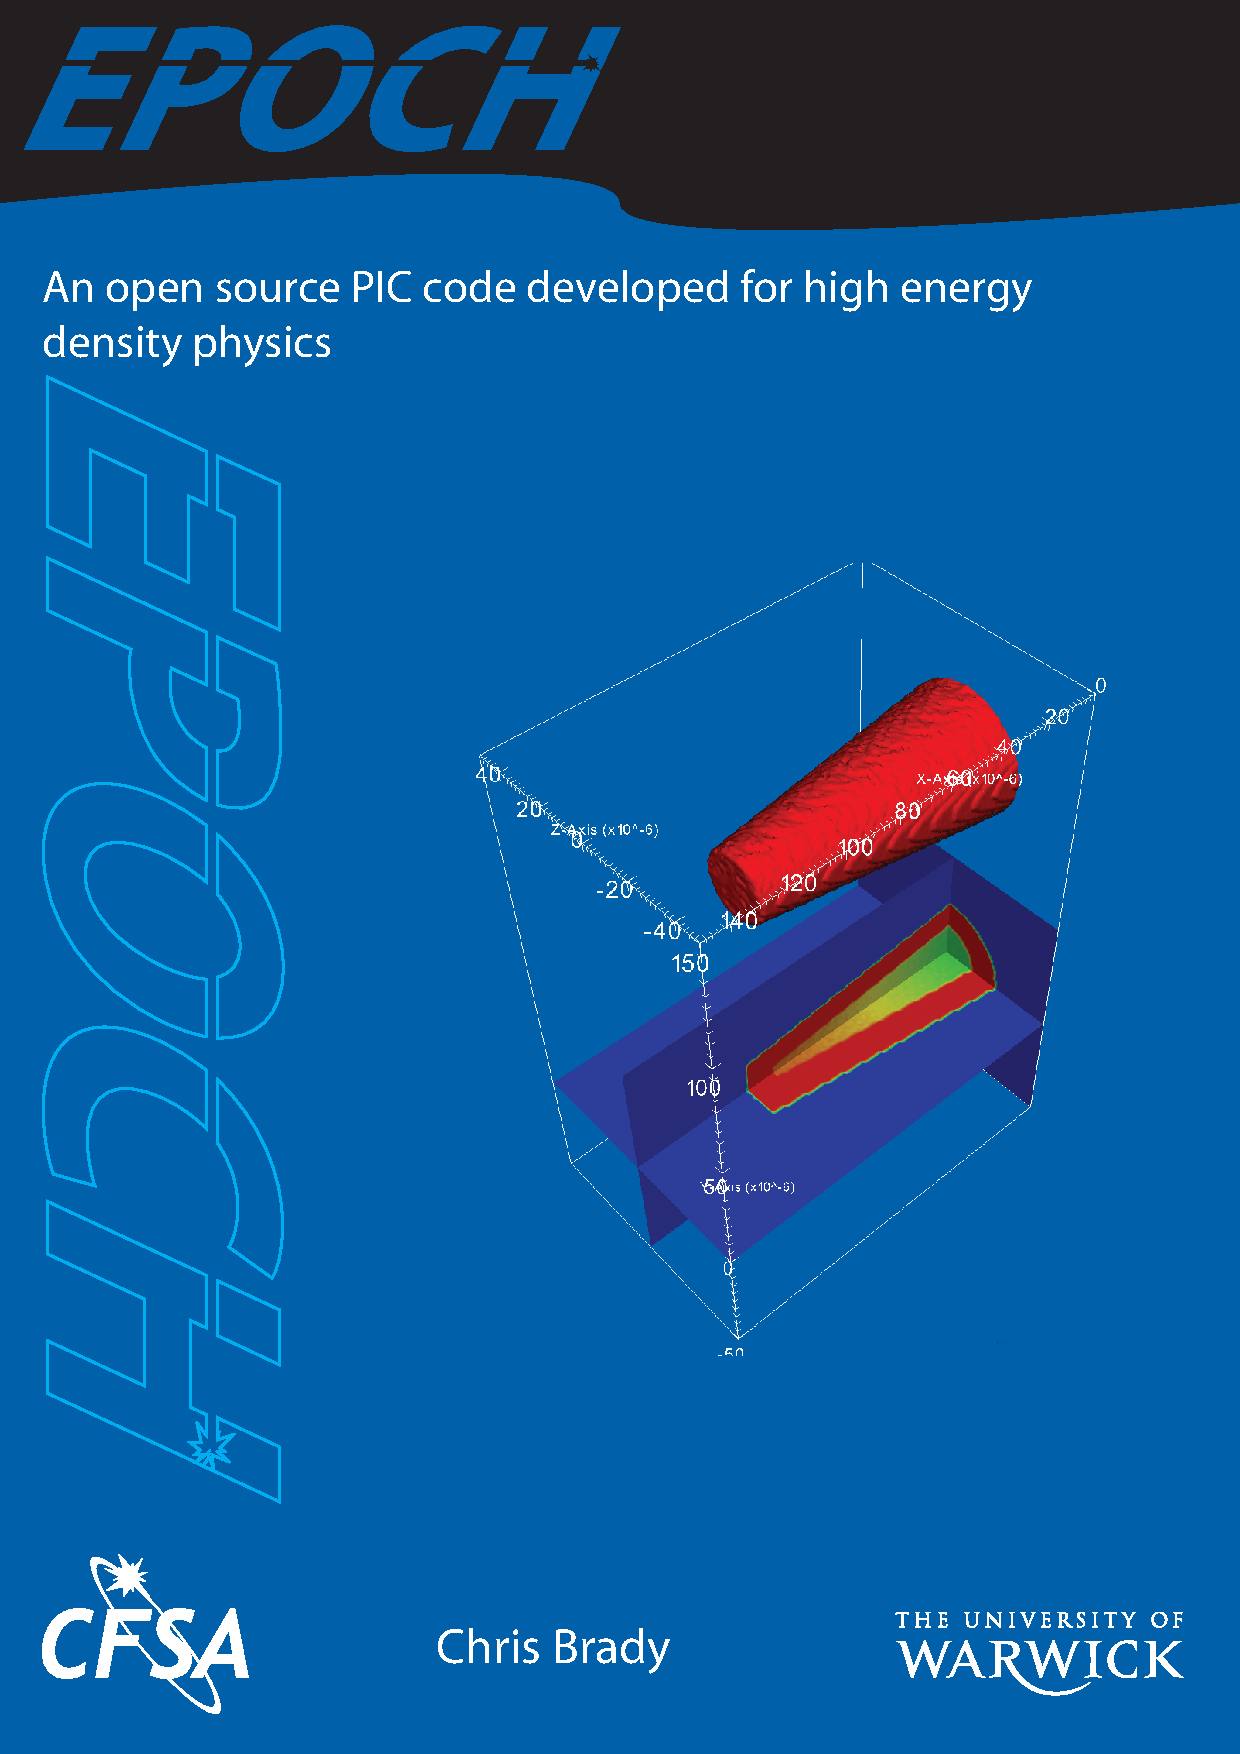
\includepdf{images/title_page_user}
{
  \fontfamily{phv}\selectfont\begin{titlepage}

\begin{center}

%This section borrows heavily from WikiBooks LaTeX

\includegraphics[width=14cm]{./images/EPOCHLogo}\\[1cm]

\textsc{\LARGE{University of Warwick}}\\[1.5cm]

% Title
\HRule\\[0.2cm]
{\huge\bfseries{Users Manual for the EPOCH PIC codes}}\\[0.4cm]
\HRule\\[1.5cm]

% Author and supervisor
\begin{minipage}{0.4\textwidth}
\begin{flushleft}\large%
\emph{Last revision by:}\\
Keith \textsc{Bennett}
\end{flushleft}
\end{minipage}
\begin{minipage}{0.4\textwidth}
\begin{flushright}\large%
\emph{EPOCH written by:} \\
Chris \textsc{Brady}\\
Keith \textsc{Bennett}\\
\end{flushright}
\end{minipage}

\vfill%
% Bottom of the page
{\large\today, {\EPOCH} Version \version}

\end{center}

\end{titlepage}

}
\fontfamily{garamond}\selectfont%
\tableofcontents%
\newpage%
\DefineShortVerb{\#}
\fvset{formatcom=\color{warwickred}}

\section{FAQs}

\subsection{What is {\EPOCH}?}

{\EPOCH} is a plasma physics simulation code which uses the Particle in Cell
(PIC) method. In this method, collections of physical particles are represented
using a smaller number of pseudoparticles, and the fields generated by the
motion of these pseudoparticles are calculated using a finite difference time
domain technique on an underlying grid of fixed spatial resolution. The forces
on the pseudoparticles due to the calculated fields are then used to update the
pseudoparticle velocities, and these velocities are then used to update the
pseudoparticle positions. This leads to a scheme which can reproduce the full
range of classical micro-scale behaviour of a collection of charged
particles.\\

\subsubsection{Features of {\EPOCH}}
\begin{itemize}
  \item MPI parallelised explicit 2nd order relativistic PIC code.
  \item Dynamic MPI load balancing option.
  \item MPI-IO based output, allowing restart on arbitrary number of processors.
  \item Data analysis and visualisation options include ITT IDL, LLNL VisIt
    and Mathworks MatLab.
  \item Control of setup and runs of {\EPOCH} through a customisable input deck.
\end{itemize}

\subsection{The origins of the code}
The {\EPOCH} family of PIC codes is based on the older code PSC by Hartmut Ruhl,
and retains almost the same core algorithm for the field updates and particle
advance routines. {\EPOCH} was written to add more modern features, and to
structure the code in such a way that future expansion of the code is made as
easy as possible.

\subsection{What normalisations are used in {\EPOCH}?}
Since the idea from the start was that {\EPOCH} would be used by a large number
of different users, and that it should be as easy as possible to ``plug in''
different modules from different people into a given copy of the code, it was
decided to write {\EPOCH} in SI units. There are a few places in the code where
some quantities are given in other units for convenience (for example charges
are specified in multiples of the electron charge), but the entire of the core
code is written in SI units.

\subsection{What are those \code{\_num} things doing everywhere?}
Historically using the compiler auto-promotion of \code{REAL} to
\code{DOUBLE PRECISION} was unreliable, so {\EPOCH} uses kind tags to specify
the precision of the code. The \code{\_num} suffixes and the associated
definition of \code{REAL}s as \code{REAL(num)} are these kind tags in
operation. The \code{\_num} tags force numerical constants to match the
precision of the code preventing errors due to precision conversion. The
important thing is that all numerical constants should be tagged with an
\code{\_num} tag, and all \code{REAL}s should be defined as \code{REAL(num)}.

\subsection{What is an input deck?}
An input deck is text file which can be used to set simulation parameters
for {\EPOCH} without needing to edit or recompile the source code.
It consists of a list of blocks which start as \inlineemph{begin:blockname}
and end with \inlineemph{end:blockname}. Within the body of each block is
a list of key/value pairs, one per line, with key and value separated by
an equals sign. Most aspects of a simulation can be controlled using an
input deck, such as the number of grid points in the simulation domain,
the initial distribution of particles and initial electromagnetic field
configuration. It is designed to be relatively easy to read and edit. For
most simulations it should be possible to set up a simulation without
editing the source code at all.

\subsection{I just want to use the code as a black box, or I'm just
  starting. How do I do that?}
\sectit{gettingstarted} There's quite a lot to learn to get started so you
should plan to read through all of this section. Then look at the code and have
a play with some test problems. After that re-read this section. This should be
enough for testing simple problems.

\subsection{I've been through the getting started guides but want more detail
  on using the code. How do I do that?}
\sectit{endusers}. Once again expect to have to read this all the way through.
Do some example problems with the code and then re-read the section.

\subsection{What is the autoloader?}
Throughout this document we will often refer to the ``autoloader'' when
setting up the initial particle distribution. In the input deck it is
possible to specify a functional form for the density and temperature 
of a particle species. {\EPOCH} will then place the particles to match
the density function and set the velocities of the particles so that they
match the Maxwellian thermal distribution for the temperature.
The code which performs this particle set up is called the ``autoloader''.

At present, there is no way to specify a non-Maxwellian particle distribution
from within the input deck. In such cases, it is necessary to edit and
recompile the {\EPOCH} source code. The recommended method for setting
the initial particle properties is to use the ``\code{manual\_load}'' function
as described in \sect{manualload}.

\subsection{What is a maths parser?}
As previously mentioned, the behaviour of {\EPOCH} is controlled using an
input deck which contains a list of key/value pairs. The value part of the
pair is not restricted to simple constants but can be a complex mathematical
expression. It is evaluated at run time using a section of code called the
"maths parser". There is no need for the end user to know anything about this
code. It is just there to enable the use of mathematical expressions in the
input deck.
Further information about this facility can be found in
\sect{maths_parser}.

\subsection{I am an advanced user, but I want to set up the code so that less
  experienced users can use it. How do I do that?}
\sectit{customising}

\subsection{I want to develop an addition to {\EPOCH}. How do I do that?}
Basically read the entire of this manual. The second part of the manual details
the internals of the code but it expects you to already be familiar with all
the material in the first part of the manual.

\subsection{I want to have a full understanding of how {\EPOCH} works. How do I
  do that?}
If you really want to understand {\EPOCH}
in full, the only way is to read all of
this manual and then read through the code. Most of it is commented.
\pagebreak

\section{Getting Started Guides}
\label{sec:gettingstarted}

\subsection{History of these guides}
These guides are based on material which was used as handouts at an {\EPOCH}
introductory workshop held in February 2010 at the University of Warwick. The
purpose of these guides is to quickly get a new user to the point of being able
to use {\EPOCH} without getting bogged down in the details of how the code
works. Some of the material covered in these getting started guides will also
appear in the body of the manual starting from \sect{endusers}.

\subsection{Running {\EPOCH} and basic control of EPOCH1D}
When the code is run, the output is
\begin{lboxverbatim}{Command line output}

     @@@@@@@@  @@@@@@      @@@@    @@@@@@@@  @@    @@    @@@@@@    @@@@@@       
     @@@@@@@@  @@@@@@      @@@@    @@@@@@@@  @@    @@    @@@@@@    @@@@@@       
     @@        @@    @@  @@    @@  @@        @@    @@      @@@@    @@  @@       
     @@        @@    @@  @@    @@  @@        @@    @@      @@@@    @@  @@       
     @@        @@    @@  @@    @@  @@        @@    @@      @@@@    @@    @@     
     @@        @@    @@  @@    @@  @@        @@    @@      @@@@    @@    @@     
     @@@@@@@@  @@@@@@    @@    @@  @@        @@@@@@@@      @@@@    @@    @@     
     @@@@@@@@  @@@@@@    @@    @@  @@        @@@@@@@@      @@@@    @@    @@     
     @@        @@        @@    @@  @@        @@    @@      @@@@    @@    @@     
     @@        @@        @@    @@  @@        @@    @@      @@@@    @@    @@     
     @@        @@        @@    @@  @@        @@    @@      @@@@    @@  @@       
     @@        @@        @@    @@  @@        @@    @@      @@@@    @@  @@       
     @@@@@@@@  @@          @@@@    @@@@@@@@  @@    @@    @@@@@@@@  @@@@@@       
     @@@@@@@@  @@          @@@@    @@@@@@@@  @@    @@    @@@@@@@@  @@@@@@       
                                                                                
                                                                                
                                                                                
                                                                                
 
 Welcome to EPOCH1D Version 3.0             
 
 The code was compiled with the following compile time options
 *************************************************************
 Per particle weighting -DPER_PARTICLE_WEIGHT
 Tracer particle support -DTRACER_PARTICLES
 Particle probe support -DPARTICLE_PROBES
 *************************************************************
 
 Code is running on 1 processing elements
 
 
 Specify output directory
\end{lboxverbatim}

At which point the end user should simply type in the name of the directory
where the code output is to be placed. This directory must also include the
file \qtt{input.deck} which controls the code setup, specifies how to set the
initial conditions and controls the I/O. Writing an input deck for {\EPOCH} is
fairly time consuming and so the code is supplied with an example input deck
which includes all the necessary sections for the code to run. This section of
the manual describes how to set up the basic code and a few simple problems in
EPOCH1D.

\subsection{\code{input.deck}}
Most of the control of {\EPOCH} is through a text file called \code{input.deck}.
The input deck file must be in the output directory and contains all the basic
information which is needed to set up the code, including the size and
subdivision of the domain, the boundary conditions, the species of particles to
simulate and the output settings for the code. For most users this will be
capable of specifying all the initial conditions and output options they need.
More complicated initial conditions will be handled in the next section.

The input deck is split into blocks of related variables. The blocks can appear
in any order. Blocks can also use variables defined in other blocks. Thus in
the examples below you must understand the roles of all blocks to understand
the full \code{input.deck}.

\subsubsection{\cemph{control} block}
The \cemph{control} block sets up the basic code properties for the
domain, the end time of the code, the load balancer and the types of initial
conditions to use.

\begin{lboxverbatim}{control block}
begin:control
   nx = 2000 # in x
   npart = 200*200*40

   nsteps = -1

   t_end = 0.3e-12

   x_min = -5e-6
   x_max = 5e-6

   # dt_multiplier = 0.95
   dlb_threshold = 1.0

   # restart_snapshot = 98

   # field_order = 2
   # stdout_frequency = 10
end:control
\end{lboxverbatim}

As illustrated in the above code block, the ``{\texttt{\#}}'' symbol is treated
as a comment character and the code ignores everything on a line following this
character.\\

{\emphtext nx} - Number of grid points in the x direction. This parameter
is mandatory. There must be sufficient gridpoints so that
(x\_max-x\_min)/nx $< \lambda_d$, where $\lambda_d$ is the Debye length.\\

{\emphtext npart} - The global number of pseudoparticles in the
simulation. This parameter does not need to be given if a specific number
of particles is supplied for each particle species. Specifying both will just
use the number of particles supplied for each species.\\

{\emphtext nsteps} - The number of iterations of the core solver before the
code terminates. Negative numbers instruct the code to only terminate at
\inlineemph{t\_end}. If \inlineemph{nsteps} is not specified then
\inlineemph{t\_end} must be given.\\

{\emphtext t\_end} - The final simulation time in simulation seconds before the
code terminates. If \inlineemph{t\_end} is not specified the
\inlineemph{nsteps} must be given. If they are both specified then
the first time restriction to be satisfied takes precedence.\\

{\emphtext x\_min} - The position of the left hand edge of the domain in
metres. Can be negative. ``x\_start'' is accepted as a synonym. This parameter
is mandatory.\\

{\emphtext x\_max} - The position of the right hand edge of the domain in
metres. Must be greater than \inlineemph{x\_min}.
``x\_end'' is accepted as a synonym. This parameter is mandatory.\\

{\emphtext dt\_multiplier} - Factor by which the timestep is multiplied before
it is applied in the code, i.e. a multiplying factor applied to the CFL
condition on the timestep. Must be less than one. If no value is given then
the default of 0.95 is used.\\

{\emphtext dlb\_threshold} - The minimum ratio of the
load on the least loaded processor to that on the most loaded processor allowed
before the code load balances. Set to 1 means
always balance, set to 0 means never balance. If this parameter is not
specified then the code will only be load balanced at initialisation time.\\

{\emphtext restart\_snapshot} - The number of a previously written restart
dump from which to restart the code. If not restarting from a previous run
this variable does not need to be set.\\

{\emphtext field\_order} - Order of the finite difference scheme used for
solving Maxwell's equations. Can be 2, 4 or 6. If not specified, the default
is to use a second order scheme.\\

{\emphtext stdout\_frequency} - If specified then the code will print a one
line status message to stdout after every given number or timesteps. The
default (\code{stdout\_frequency = 0}) is to print nothing to screen.

\subsubsection{\inlineemph{boundaries} block}
The {\emphtext boundaries} block sets the boundary conditions of each boundary
of the domain. Some types of boundaries allow EM wave sources (lasers) to be
attached to a boundary. Lasers are attached at the initial conditions
stage.

\begin{lboxverbatim}{boundaries block}
begin:boundaries
   bc_x_min = simple_laser
   bc_x_max_field = simple_outflow
   bc_x_max_particle = simple_outflow
end:boundaries
\end{lboxverbatim}

{\emphtext bc\_x\_min} - The condition for the left boundary for both fields
and particles. ``xbc\_left'' is accepted as a synonym.\\

{\emphtext bc\_x\_min\_\{field,particle\}} - The condition for the left
boundary for \{fields,particles\}.\linebreak ``xbc\_left\_\{field,particle\}''
is accepted as a synonym.\\

{\emphtext bc\_x\_max} - The condition for the right boundary for both fields
and particles. ``xbc\_right'' is accepted as a synonym.\\

{\emphtext bc\_x\_max\_\{field,particle\}} - The condition for the right
boundary for \{fields,particles\}.\linebreak ``xbc\_right\_\{field,particle\}''
is accepted as a synonym.\\

There are six boundary types in {\EPOCH} and each boundary of the domain can
have one and only one of these boundaries attached to it. These boundary types
are:\\

{\emphtext periodic} - A simple periodic boundary condition. Fields and/or
particles reaching one edge of the domain are wrapped round to the opposite
boundary.\\

{\emphtext other} - A generic boundary condition which in the default {\EPOCH}
version is perfectly reflecting for both particles and EM waves.\\

{\emphtext simple\_laser} - A characteristic based boundary condition to which
one or more EM wave sources can be attached. Since the wave sources require the
domain to be completely set up before they can be calculated the wave sources
are attached when the initial conditions are set.  EM waves impinging on a
\inlineemph{simple\_laser} boundary are transmitted with as little reflection
as possible. Particles are fully transmitted. The field boundary condition
works by allowing outflowing characteristics to propagate through the boundary
while using the attached lasers to specify the inflowing characteristics. The
particles are simply removed from the simulation when they reach the
boundary.\\

{\emphtext simple\_outflow} - A simplified version of \inlineemph{simple\_laser}
which has the same properties of transmitting incident waves and
particles, but which cannot have EM wave sources attached to it. These
boundaries are about 5\% more computationally efficient than
\inlineemph{simple\_laser boundaries} with no attached sources. This boundary
condition again allows outflowing characteristics to flow unchanged, but this
time the inflowing characteristics are set to zero. The particles are again
simply removed from the simulation when they reach the boundary.\\

{\emphtext reflect} - A perfectly reflecting boundary condition.\\

{\emphtext open} - When applied to fields, EM waves outflowing characteristics
propagate through the boundary. Particles are transmitted through the boundary
and removed from the system.\\

{\emphtext NOTE: If simple\_laser, simple\_outflow or open are specified on
one or more boundaries then the code will no longer necessarily conserve mass.}

Note also that it is possible for the user to specify contradictory,
unphysical boundary conditions. It is the users responsibility that these
flags are set correctly.

\subsubsection{\inlineemph{species} block}

\begin{lboxverbatim}{species block}
begin:species
   # electrons
   name = Electron
   charge = -1.0
   mass = 1.0
   frac = 0.5
   # npart = 2000*100
   dump = T
   # tracer = F
   number_density = 1.e4
   temp = 1e6

   temp_x = 0.0
   temp_y = temp_x(Electron)
   number_density_min = 0.1 * den_max
   number_density = if(abs(x) lt thick,den_max,0.0)
   number_density = if((x gt -thick) and (abs(y) gt 2e-6),0.0,number_density(Carbon))
end:species

begin:species
   # carbon4+
   name = Carbon
   charge = 4.0
   mass = 1836.0*12
   frac = 0.5
   # npart = 2000*100
   dump = T

   number_density = 0.25*number_density(Electron)
   temp_x = temp_x(Electron)
   temp_y = temp_x(Electron)
end:species
\end{lboxverbatim}

{\emphtext name} - This specifies the name of the particle species defined
in the current block. This name can include any alphanumeric characters in
the basic ASCII set. The name is used to identify the species in any
consequent input block. It is a mandatory parameter.\\

{\emphtext NOTE: IT IS IMPOSSIBLE TO SET TWO SPECIES WITH THE SAME NAME!} \\

{\emphtext charge} - This sets the charge of the species in
multiples of the electron charge. Negative numbers are used for negatively
charged particles. This is a mandatory parameter.\\

{\emphtext mass} - This sets the mass of the species in multiples
of the electron mass. Negative numbers are not trapped and effectively swap the
charge of the species. This is not recommended since it breaks the
mass\_density diagnostic. This is a mandatory parameter.\\

{\emphtext npart} - This specifies the number of pseudoparticles
which should be loaded into the simulation domain for the species. This is the
most convenient way of loading particles for simulations containing multiple
species with different number densities. If these are specified then
\inlineemph{npart} (the global number of particles specified in the control
block) is ignored for this species. It should not be specified at the same time
as frac for a given species.\\

{\emphtext frac} - This specifies what fraction of npart (the
global number of particles specified in the control block) should be assigned
to the species.\\

{\emphtext NOTE: frac should not be specified at the same time as npart for a
given species.}\\

{\emphtext dump} - Logical flag detailing whether or not to dump
information about the species. If set to ``F'', then the species information
is not dumped when writing ANY species specific diagnostics, although it is
included in global diagnostics (i.e in the example if ``dump = F'' were
specified then there would be no ``Mass\_Density\_Electron'', but the mass of
the electron would be considered when calculating ``mass\_density'') and
restart dumps. ``dump = F'' is the default value.\\

{\emphtext tracer} - Logical flag switching the particle species
into tracer particles. Tracer particles are enabled with the correct
precompiler option, and when set for a given species make that species move
correctly for its charge and mass, but contribute no current. This means that
these particles are passive tracers in the plasma. ``tracer = F'' is the
default value.\\

The species blocks are also used for specifying initial conditions for
the particle species. The initial conditions in {\EPOCH} can be specified in
various ways, but the easiest way is to specify the initial conditions in the
input deck file. This allows any initial condition which can be specified
everywhere in space by a number density and a drifting Maxwellian distribution
function.
These are built up using the normal maths
expressions, by setting the density and temperature for each species which is
then used by the autoloader to actually position the particles. \\
The elements of the species block used for setting
initial conditions are:\\

{\emphtext number\_density} - Particle number density in $m^{-3}$.
As soon as a number\_density= line has been read, the values are
calculated for the whole domain and are available for reuse on the right hand
side of an expression. This is seen in the above example in the first two lines
for the carbon species, where the density is first set and then corrected.\\
This parameter is mandatory.\\

{\emphtext number\_density\_min} - Minimum particle number density in $m^{-3}$.
When the number density in a cell falls below number\_density\_min the
autoloader does not load any pseudoparticles into that cell to minimise the
number of low weight, unimportant particles. If set to 0 then all cells are
loaded with particles. This is the default.\\

{\emphtext number\_density\_max} - Maximum particle number density in $m^{-3}$.
When the number density in a cell rises above number\_density\_max the
autoloader clips the density to number\_density\_max allowing easy
implementation of exponential rises to plateaus. If it is a negative value
then no clipping is performed. This is the default.\\

{\emphtext temp\_\{x,y,z\}} - The temperature in each direction for a thermal
distribution in K. To specify a temperature in ev, simply use the deck
parser. So for example temp\_x = 4*kev/kb gives a 4kev temperature.\\

{\emphtext temp} - Sets an isotropic temperature distribution in K. Does not
give thermal distribution in ignorable directions. If both temp and a specific
temp\_x, temp\_y, temp\_z parameter is specified then the last to appear in the
deck has precedence. If neither are given then the species will have a default
temperature of zero Kelvin.\\

{\emphtext temp\_\{x,y,z\}\_ev, temp\_ev} - These are the same as the
temperature parameters described above except the units are given in
electronvolts rather than Kelvin.\\

{\emphtext drift\_\{x,y,z\}} - Specifies a momentum space offset in
$kg\ ms^{-1}$ to the distribution function for this species. By default,
the drift is zero.\\

It is also possible to set initial conditions for a particle species
using an external file.  Instead of specifying the
initial conditions mathematically in the input deck, you specify in quotation
marks the filename of a simple binary file containing the information required.

\begin{lboxverbatim}{external initial conditions}
begin:species
   name = Electron
   number_density = 'Data/ic.dat'
   offset = 80000
   temp_x = 'Data/ic.dat'
end:species
\end{lboxverbatim}


An additional element is also introduced, the offset element. This
is the offset in bytes from the start of the file to where the data should
be read from. As a given line in the block executes, the file is opened, the
file handle is moved to the point specified by the offset parameter, the data
is read and the file is then closed. Therefore, unless the offset value is
changed between data reading lines the same data will be read into all the
variables. The data is read in as soon as a line is executed, and so it is
perfectly possible to load data from a file and then modify the data using
a mathematical expression.\\

The file should be a simple binary file consisting of floating point numbers of
the same precision as \inlinecode{\_num} in the core {\EPOCH} code.\\

{\emphtext NOTE: The files that are expected by this block are SIMPLE BINARY
files, NOT Fortran unformatted files. It is possible to read Fortran
unformatted files using the offset element, but care must be taken!}\\


\subsubsection{\inlineemph{output} block}
\label{sec:output block}
Output in {\EPOCH} is handled using the custom designed SDF file format
(\inlineemph{Self Describing Format}) which is documented in \sect{sdf}
of the developers manual.
It comes with readers for ITT IDL and LLNL VisIt, and Mathworks MatLab.
The IDL reader is also compatible with the open source GDL tool.
What the code should output and when it should output it is
specified in the ``output'' block of the input deck. \\

There are three types of output dump in {\EPOCH} which are used for different
purposes. These types are:\\

{\emphtext normal} - The most frequent type of output dump in {\EPOCH} is a
normal dump.\\

{\emphtext full} - A full dump is usually written every 10 or so normal
dumps. A full dump contains all the data that a normal dump contains and should
also contain any information which is needed only infrequently, whether this is
the full particle information or a large distribution function. It is possible
to turn off full dumps completely.\\

{\emphtext restart} - A restart dump is a dump where the code guarantees to
write enough data to allow the code to restart from the output. Output dumps
are guaranteed to contain all the information in a normal dump and, if they
coincide with the timing for a full dump, will also contain the full dump
information.\\

Information will never be written into a file twice, even if two conditions for
it being written are satisfied (i.e even if px should be dumped both because it
is a full dump and a restart dump, px will only be written once).\\

When specifying which type of output dump to write a variable to there are four
options which are specified for each variable and can be combined by
addition. Some combinations make no sense but are formally
valid. These are:\\

{\emphtext never} - If the variable is not a required restart variable then it
will never be written. If it is a required restart variable then it will be
written only at restart dumps.\\

{\emphtext always} - This variable will be written at full, normal and restart
dumps.\\

{\emphtext full} - This variable will be written at full dumps only.\\

{\emphtext restart} - This variable will be written at restart dumps only.\\

There is also a fifth parameter which can be specified for some variables.\\

{\emphtext species} - The output for this variable should be broken down on a
species by species basis. This only applies to certain kinds of derived field
variable, such as mass\_density. It is combined with a restart frequency code
by addition as in: \inlinecode{px = always + species}.\\

When applied to a variable, these codes are referred to as a
\inlineemph{dumpmask}.

\begin{lboxverbatim}{output block}
begin:output
   # If use_offset_grid is true then the code dumps a grid which
   # displays positions relative to the left hand edge of the window
   use_offset_grid = F
   # number of timesteps between output dumps
   dt_snapshot = 1.0e-14
   # Number of dt_snapshot between full dumps
   full_dump_every = 10
   restart_dump_every = -1
   force_final_to_be_restartable = T

   # Properties at particle positions
   particles = never
   px = never
   py = never
   pz = never
   vx = never
   vy = never
   vz = never
   charge = never
   mass = never
   particle_weight = never
   species_id = never

   # Properties on grid
   grid = always
   ex = always
   ey = always
   ez = always
   bx = always
   by = always
   bz = always
   jx = always
   jy = always
   jz = never
   ekbar = always + species
   mass_density = never + species
   charge_density = always
   number_density = always + species
   temperature = always + species

   distribution_functions = always
   particle_probes = never
end:output
\end{lboxverbatim}

{\emphtext use\_offset\_grid} - When using moving windows some visualisation
programs (notably VisIt) show the motion of the window by moving the
visualisation window rather than by changing the x-axis. Setting this option to
``T'' causes the code to write another grid which always gives the offset
relative to the left hand edge of the window rather than the true origin.
Performs no function when not using the moving window. The default value
is ``F''.\\

{\emphtext dt\_snapshot} - Sets the interval between normal output dumps in
simulation seconds. Setting zero or negative means that the code will output
every step of the core solver. The code does NOT guarantee that outputs will be
exactly \inlineemph{dt\_snapshot} apart, what is guaranteed is that the next
output will be after the first iteration which takes the simulation to a time
$\ge$ \inlineemph{dt\_snapshot} from the last output. The default value is
larger than the length of the simulation that will never trigger an output.\\

{\emphtext nstep\_snapshot} - Sets the number of timesteps between normal
output dumps. Setting zero or negative means that the code will output
every step of the core solver. If \inlineemph{dt\_snapshot} is also specified
then both conditions are considered. The default value is a huge integer
which will never trigger an output.\\

{\emphtext full\_dump\_every} - The number of normal output dumps between full
output dumps. Setting to zero makes every dump a full dump. Setting to a
negative number stops the code from producing any full dumps. This is the
default.\\

{\emphtext restart\_dump\_every} - The number of normal output dumps between
restart dumps. Setting to zero makes every dump a restart dump. Setting to a
negative number stops the code from producing any restart dumps. This is the
default.\\

{\emphtext force\_final\_to\_be\_restartable} - Force the code to override
other output settings and make the last output dump it writes be a restart
dump. Any internal condition which causes the code to terminate will make the
code write a restart dump, but code crashes or scheduler terminations will not
cause the code to write a restart dump. The default value is ``T''.\\

{\emphtext dump\_source\_code} - {\EPOCH} has the ability to write its own
source code into restart dumps. This is generated at compile time and embedded
into the binary and so is guaranteed to match that corresponding to the running
code. {\EPOCH} comes with a script called
\inlineemph{unpack\_source\_from\_restart} which can be used to unpack the
source code from a restart dump. If this logical flag is set to false then 
the feature will be disabled. The default value is ``T''.\\

{\emphtext dump\_input\_decks} - If this logical flag is set to true then
a copy of the input decks for the currently running simulation is written
into the restart dumps. The default value is ``T''.\\

{\emphtext particles} - The dumpmask for the particle positions. Restart
variable. No particle variables can be plotted in VisIt unless this is
dumped.\\

{\emphtext p\{x,y,z\}} - The dumpmasks for the particle momenta. Restart
variable.\\

{\emphtext v\{x,y,z\}} - The dumpmasks for the particle velocities.\\

{\emphtext charge} - The dumpmask for the charge of a given particle. This
has no effect if the code is not compiled with the option for per particle
charge. See details on the \code{Makefile} later.\\

{\emphtext mass} - The dumpmask for the mass of a given particles. This
has no effect if the code is not compiled with the option for per
particle mass.\\

{\emphtext particle\_weight} - The dumpmask for the weighting function which
describes how many real particles each pseudoparticle represents. Restart
variable.\\

{\emphtext species\_id} - The dump mask for the number representing which
particle species a given particle is. This is the same as the number assigned
to that particle species in the species block. Restart variable.\\

{\emphtext grid} - The dumpmask for the Cartesian grid which defines the
locations of the grid variables. No grid variables can be plotted in VisIt
unless this variable is output.\\

{\emphtext e\{x,y,z\}} - The electric field vectors pointing in all three
directions. Restart variables.\\

{\emphtext b\{x,y,z\}} - The magnetic field vectors pointing in all three
directions. Restart variables. In 1D bx is a trivial variable because of the
Solenoidal condition. It is included simply for symmetry with higher dimension
codes.\\

{\emphtext j\{x,y,z\}} - The currents pointing in all three directions. Restart
variables.\\

{\emphtext ekbar} - Mean kinetic energy on grid. Can have species dumpmask.\\

{\emphtext mass\_density} - Mass density on grid. Can have species dumpmask.\\

{\emphtext charge\_density} - Charge density on grid. Can have species
dumpmask.\\

{\emphtext number\_density} - Number density on grid. Can have species
dumpmask.\\

{\emphtext temperature} - Temperature on grid. Can have species dumpmask. The
exact way that temperature is calculated in the code is likely to vary in the
near future.\\

{\emphtext distribution\_functions} - Dumpmask for outputting distribution
functions specified in the input deck. Each individual distribution function
can have its own dumpmask, but this one takes precedence.\\

{\emphtext particle\_probes} - Dumpmask for outputting particle probes
specified in the input deck. Each individual particle probe
can have its own dumpmask, but this one takes precedence.\\

% fix: ejected_particles

\subsection{\inlineemph{constant} blocks}

The \inlineemph{constant} block type helps to make the input deck more flexible
and maintainable. It allows you to define constants and maths parser
expressions which can be used by name later in the deck.\\

Constants are simply maths parser expressions which are assigned to a name as
shown above. When the name is used on the right hand side of a deck expression
it is replaced by the expression it was assigned with. This expression may
be a simple numerical constant, a mathematical expression or a function.
Constants may contain spatially varying information without having to
pre-calculate them at every location in the domain.
To those familiar with old Fortran codes, constants are essentially just
statement functions.\\

If a constant name is reused in a constant block then the old constant is
deleted and replaced with the new one. This happens without warning.\\

\begin{lboxverbatim}{constant block}
begin:constant
   lambda = 1.0e-6 # 1 micron wavelength
   omega = 2.0*pi*c/lambda
   den_crit = critical(omega)
   scale = 3.5e-6 # microns
   den_max = 5.0*den_crit
   thick = 300e-9
   pplength = 6000e-9
   widscale = 5.0e-6

   t_wid = (10.0e-6)/c
   amax = 1.0
   wy = 1e-6
   y = 0.0

   slope = exp(-2.0*(y/wy)^2)
   blob = gauss(sqrt(x^2+y^2),0.0,1.0e-6)
end:constant
\end{lboxverbatim}

Using constants can be very helpful when dealing with long,
complicated expressions since they allow the expression to be broken down into
much simpler parts. They can also be used to get around the Fortran string
length limitation built into many compilers which prevents deck lines being
longer then 512 characters long. As a general rule, it is a good idea to break
down complicated expressions using constants or by other means, in order to
make the deck look more readable.\\

Constants are persistent for the entire runtime of the code,
allowing them to be used when specifying time profiles for lasers, and also
allowing developers to use maths parser expressions for other internal parts of
the code where needed.\\

In the above example, several pre-defined constants have been used
(\inlineemph{pi} and \inlineemph{c}) and also several functions
(\inlineemph{critical}, \inlineemph{exp}, \inlineemph{gauss} and
\inlineemph{sqrt}). These are described in \sect{constants} and
\sect{functions}.

\subsubsection{\inlineemph{laser} blocks}
\label{sec:lasers}
Laser blocks attach an EM wave source to a boundary which is set as
\inlineemph{simple\_laser}.

\begin{lboxverbatim}{laser block}
begin:laser
   boundary = x_min
   id = 1
   irradiance_w_cm2 = 1.0e15
   lambda = 1.06 * microns
   pol_angle = 0.0
   phase = 0.0
   t_profile = gauss(time,40.0e-15,40.0e-15)
   t_start = 0.0
   t_end = 80.0e-15
end:laser
\end{lboxverbatim}

As already mentioned in the discussion of laser boundaries in the boundaries
block, lasers are attached to compatible boundaries here in the initial
conditions deck. In 1D, laser blocks are slightly simpler than their 2D and 3D
equivalents, but most of the important features will be mentioned here. The
only significant difference is that there is also a spatial profile for
multidimensional lasers. This is covered in detail in
\sect{multilaser}.\\

{\emphtext boundary} - The boundary on which to attach the laser.
In 1D, the directions can be either x\_min or x\_max.  ``left'' and ``right''
are accepted as a synonyms for ``x\_min'' and ``x\_max''.\\

{\emphtext amp} - The amplitude of the $E$ field of the laser in $V/m$.\\

{\emphtext irradiance} - The irradiance (intensity) of the laser in $W/m^2$.
There is no need to specify both irradiance and amp and the last specified
in the block is the value used. It is mandatory to specify at least one.\\

{\emphtext irradiance\_w\_cm2} - This is identical to the 
\inlineemph{irradiance} parameter described above, except that the units
are specified in $W/cm^2$.\\

{\emphtext id} - An id code for the laser. Used if you specify the laser time
profile in the {\EPOCH} source rather than in the input deck. Does not have to
be unique, but all lasers with the same id will have the same time profile.
This parameter is optional and is not used under normal conditions.\\

{\emphtext omega} - Angular frequency (rad/s not Hz) for the laser.\\

{\emphtext lambda} - Wavelength in a vacuum for the laser specified in $m$.
If you want to specify in $\mu m$ then you can multiply by the constant
``microns''. One of \inlineemph{lambda} or \inlineemph{omega} is a
required parameter.\\

{\emphtext pol\_angle} - Polarisation angle for the laser in radians.
This parameter is optional and has a value of zero by default.
The angle is measured with respect to the right-hand triad of propagation
direction, electric and magnetic fields. Although the 1D code has no $y$
or $z$ spatial axis, the fields still have $y$ and $z$ components.
If the laser is on \inlineemph{x\_min} then the default $E$ field is in
the $y$-direction and the $B$ field is the $z$-direction. The polarisation
angle is measured clockwise about the $x$-axis with zero along the $E_y$
direction. If the laser is on \inlineemph{x\_max} then the angle is
anti-clockwise.\\

{\emphtext pol} - This is identical to \inlineemph{pol\_angle} with the angle
specified in degrees rather than radians. If both are specified then the
last one is used.\\

{\emphtext phase} - Phase shift for the laser in radians. 
There is zero phase shift applied by default.\\

{\emphtext profile} - This parameter is a little redundant in 1D and is
only included for consistency with 2D and 3D versions of the code.
The laser field is multiplied by this parameter to give its final amplitude
so the intention is to use a value between zero and one. By default it is a
unit constant and therefore has no affect on the laser amplitude.\\

{\emphtext t\_profile} - Used to specify the time profile for the laser
amplitude. Like \inlineemph{profile} the laser field is multiplied by
this parameter but it is a function of time rather than space. In a similar
manner, it is best to use a value between zero and one.
Setting values greater than one is possible but will cause the maximum laser
intensity to grow beyond \inlineemph{amp}. The default is to leave the
laser unchanged over time.\\

{\emphtext t\_start} - Start time for the laser in seconds. Can be set to the
string ``start'' to start at the beginning of the simulation. This is the
default value. When using this parameter, the laser start is hard. To get a
soft start use the \inlineemph{t\_profile} parameter to ramp the laser up to
full strength.\\

{\emphtext t\_end} - End time for the laser in seconds, can be set to the
string ``end'' to end at the end of the simulation. This is the default value.
When using this parameter, the laser end is clipped straight to zero at
t$>$\inlineemph{t\_end}. To get a soft end use the \inlineemph{t\_profile}
parameter to ramp the laser down to zero.\\

In theory, any laser time profile required is possible, but the core FDTD
solver for the EM fields in {\EPOCH} produces spurious results if sudden
changes in the field intensity occur. This is shown in Figures~\ref{badpulse}
and \ref{smoothpulse}. The pulse shown in Figure~\ref{badpulse} used a constant
\inlineemph{t\_profile} and used \inlineemph{t\_end} to stop the laser after
8fs. Since the stopping time was not an exact multiple of the period, the
result was to introduce spurious oscillations behind the pulse. If the laser
had a finite phase shift so that the amplitude did not start at zero, a
similar effect would be observed on the front of the pulse.

\captionedimage{./images/pulse2}{badpulse}{A laser pulse with a sharp
  cutoff shows numerical artifacts behind the pulse.}
\captionedimage{./images/pulse1}{smoothpulse}{A laser pulse with a smooth
  temporal profile shows no artifacts.}

Figure~\ref{smoothpulse} instead used a Gaussian window function with a
characteristic width of 8fs as well as using \inlineemph{t\_end} to introduce
a hard cutoff. It can clearly be seen that there are no spurious oscillations
and the wave packet propagates correctly, showing only some dispersive
features.

There is no hard and fast rule as to how rapid the rise or fall for a laser can
be, and the best advice is to simply test the problem and see whether any
problems occur. If they do then there are various solutions. Essentially, the
timestep must be reduced to the point where the sharp change in amplitude can
be accommodated. The best solution for this is to increase the spatial
resolution (with a comparable increase in the number of pseudoparticles), thus
causing the timestep to drop via the CFL condition.

This is computationally expensive, and so a cheaper option is simply to
decrease the input.deck option \inlineemph{dt\_multiplier}. This artificially
decreases the timestep below the timestep calculated from the internal
stability criteria and allows the resolution of sharp temporal gradients. This
is an inferior solution since the FDTD scheme has increased error as the
timestep is reduced from that for EM waves. The latest version of {\EPOCH}
includes a high order field solver to attempt to reduce this.

\subsubsection{\inlineemph{fields} block}
\begin{lboxverbatim}{fields block}
begin:fields
   ex = sin(pi*x/length_x)
   ey = cos(pi*x/length_x)
   ez = 0
   bx = 1.0
   by = -1.0
   bz = 0
end:fields
\end{lboxverbatim}

Note this example uses $\pi$ and length\_x. These will be explained later in
detail. The constant $\pi$, along with other constants is always available
within the input deck. The domain size length\_x, along with other useful
quantities, is calculated by the code (from x\_max and x\_min)
when it reads the input deck.

The final type of block in the {\EPOCH} input deck is the fields block. This
allows you to specify the electric and magnetic fields at any point in the
domain. Once again, this is a very simple block needing only limited
explanation. All field variables are accessible by name and can be read back
using the appropriate commands from the maths parser. \\

Any valid maths parser expression can be used to set up the fields, and no
check is made to ensure that the $\nabla.B = 0$ is satisfied. \\

\subsection{Moving to EPOCH2D and EPOCH3D}
EPOCH1D is the simplest version of {\EPOCH} and, although feature complete,
lacks many of the elements which are required for multidimensional operation.
These elements are mainly small modifications to the concepts already
introduced in EPOCH1D but are significant enough to need at least some
discussion.\\

The higher dimension versions of the code go by the uninspired names of EPOCH2D
and EPOCH3D. Most of the input decks are equivalent to those already covered in
EPOCH1D, with a few added elements for setting the number of grid points in the
additional dimensions, setting the start and end points for the axes in the new
dimensions, and setting boundary conditions on the new boundaries. These will
be covered in more detail over the next few pages.\\

The laser blocks become slightly more complicated by the addition of spatial
profiles for the laser front, and the addition of the ability to have spatially
dependent phase profiles across the laser front. This will be covered later in
this document.\\

The data loading routines are identical to those for EPOCH1D, although
obviously new routines are required to actually visualise 2D and 3D data. 2D
and 3D data is much larger than 1D, and a much larger number of particles are
required to adequately resolve the physics in multidimensional simulations. As
a consequence, the data files generated by higher dimensionality versions of
{\EPOCH} will be much larger, making the more advanced I/O routines available
in {\EPOCH} more useful. These will be covered in the following sections.\\

\subsubsection{Changes to the \inlineemph{control} block}

\begin{lboxverbatim}{Changed control block}
begin:control
   .
   .
   ny = 200
   nz = 200
   .
   y_min = -10e-6
   y_max = 10e-6
   z_min = -10e-6
   z_max = 10e-6
   .
   .
end:control
\end{lboxverbatim}

The modified control block in EPOCH2D and 3D is very similar to the control
block already introduced for EPOCH1D. All that is added are new elements
describing the number of gridpoints in y and z (\inlineemph{ny \& nz}), and
new start and end lines for the length of the domain in the new directions
(\inlineemph{y\_min $\rightarrow$ y\_max} \&
\inlineemph{z\_min $\rightarrow$ z\_max}). These operate in exactly the same
way as those already introduced with EPOCH1D.  However, care must be taken to
increase the number of particles, ensuring that the number of particles per
cell remains high enough to accurately resolve the distribution function.\\

Also note that the amount of memory required for multidimensional simulations
will generally be hundreds of times larger than that required for 1D
simulations.\\

\subsubsection{Changes to the \inlineemph{boundaries} block}

\begin{lboxverbatim}{Changed boundaries block}
begin:boundaries
   .
   .
   bc_y_min = periodic
   bc_y_max = periodic
   bc_z_min = simple_laser
   bc_z_max = simple_outflow
end:boundaries
\end{lboxverbatim}

The modified boundary block includes new boundary conditions for the additional
boundaries that are introduced in higher dimensions. These available boundaries
are exactly the same as in 1D, with the additional boundaries being:\\

\begin{tabular}{rcl}
{\inlineemtt bc\_y\_min} &-& bottom of domain. ``ybc\_down'' is also accepted.\\
{\inlineemtt bc\_y\_max} &-& top of domain. ``ybc\_up'' is also accepted.\\
{\inlineemtt bc\_z\_min} &-& back of domain. ``zbc\_back'' is also accepted.\\
{\inlineemtt bc\_z\_max} &-& front of domain. ``zbc\_front'' is also accepted.\\
\end{tabular} \\

These are equivalent to the existing 1D simulations except that the moving
window always moves parallel to the x-axis when activated.\\
This concludes all
the modifications to input.deck that are required to use {\EPOCH} in multiple
dimensions. There are some changes that are required to allow
multidimensional initial conditions, but a surprising number of initial
conditions are in fact 1D even when running in multi-dimensional versions of
{\EPOCH}. The next few pages cover the modifications to the initial conditions
file which are needed for true multidimensional initial conditions with
examples.

\subsubsection{Multidimensional initial conditions}

The basic modification to the {\EPOCH} initial conditions deck is the addition
of the new variables describing positions and length in the new directions. The
names of these variables are given in the full manual and will be used without
introduction here.

\scaledcapimage{./images/gaussic}{gaussblob}{A Gaussian density blob at the
  centre of the domain.}{0.4}

A very simple problem to set up using EPOCH2D is a Gaussian blob which is
shown in Figure~\ref{gaussblob}, in the form both of the ic.deck needed to
create it and the output from VisIt that is produced from running this deck.

\scaledcapimage{./images/invgaussic}{inversegaussblob}{A Gaussian density
  deficit at the centre of the domain.}{0.4}

In Figure~\ref{inversegaussblob}, a very small modification to this initial
conditions deck is shown which creates the a case with a Gaussian density
minimum at the centre. This makes it clear that multidimensional initial
conditions are only a little more complex than 1D initial conditions, but at
present these are not very interesting initial conditions.

The next example extends this to a more useful initial condition.\\

\begin{nbboxverbatim}{species block to set up Gaussian density blob}
begin:constant
   width = 2.5e-6 # 2.5 microns
   r = sqrt(x^2+y^2)
end:constant

begin:species
   name = Electron
   number_density = 1.0e19 * gauss(r,0.0,width)
end:species
\end{nbboxverbatim}
%
%\begin{minipage}{\textwidth}
\begin{nbboxverbatim}{species block to set up Gaussian density blob}
begin:constant
   width = 2.5e-6 # 2.5 microns
   r = sqrt(x^2+y^2)
end:constant

begin:species
   name = Electron
   number_density = 1.0e19 * (1.0-gauss(r,0.0,width))
end:species
\end{nbboxverbatim}
%\end{minipage}

\subsubsection{\inlineemph{laser} blocks in multiple dimensions.}
\label{sec:multilaser}

The laser blocks already introduced in EPOCH1D are still present in
2D and 3D, but some of the parameters now accept spatial information.\\

\scaledcapimage{./images/profile_flat}{flatlaser}{Constant laser profile}{0.4}

{\emphtext profile} - The spatial profile for the laser. This is
essentially an array defined along the edge (or surface) that the laser is
attached to. It is clear that the spatial profile is only meaningful
perpendicular to the laser's direction of travel and so it is just a single
constant in 1D. The laser profile is evaluated as an initial condition
and so cannot include any temporal information which must be
encoded in \inlineemph{t\_profile}.  The spatial profile is evaluated at the
boundary where the laser is attached and so only spatial information in the
plane of the boundary is significant. This is most clearly explained through a
couple of examples. In these examples the spatial profile of the laser is set
to vary between a flat uniform profile (\inlineemph{profile = 1}) and a
Gaussian profile in y (\inlineemph{profile = gauss(y,0,2.5e-6)}). The
difference between these profiles is obvious but the important point is that a
laser travelling parallel to the x-direction has a profile in the y
direction. Similarly a laser propagating in the y-direction has a profile in
the x direction. In 3D this is extended so that a laser propagating in a
specified direction has a profile in both orthogonal directions. So a laser
travelling parallel to the x axis in 3D would have a profile in y and z. Since
3D lasers are very similar to 2D lasers, they will not be considered here in
greater detail, but in 3D, it is possible to freely specify the laser profile
across the entire face where a laser is attached.\\

\scaledcapimage{./images/profile_gauss}{gausslaser}{Gaussian laser profile}{0.4}

{\emphtext phase} - Phase shift for the laser in radians. This is a spatial
variable which is also defined across the whole of the boundary on which the
laser is attached. This allows a user to add a laser travelling at an angle
to a boundary as shown in Figure~\ref{angle}.
\scaledcapimage{./images/wave}{wave}{Laser at an angle}{0.4}
The setup for this is not entirely straightforward and requires a little
bit of explanation. Figure~\ref{wave} illustrates a laser being driven at
an angle on the x\_min boundary. Different wave fronts cross the $y$-axis
at different places and this forms a sinusoidal profile along $y$ that
represents the phase. The wavelength of this profile is
given by $\lambda_\phi = \lambda / \sin\theta$, where $\lambda$ is the
wavelength of the laser and $\theta$ is the angle of the propagation
direction with respect to the $x$-axis. The actual phase to use will
be $\phi(y) = -k_\phi y = -2\pi y / \lambda_\phi$. It is negative because
the phase of the wave is propagating in the positive $y$ direction.
It is also necessary to alter the wavelength of the driver since this
is given in the direction perpendicular to the boundary. The new
wavelength to use will be $\lambda\cos\theta$. Figure~\ref{angle} shows
the resulting $E_y$ field for a laser driven at an angle of $\pi / 8$. Note
that since the boundary conditions in the code are derived for propagation
perpendicular to the boundary, there will be artifacts on the scale of the
grid for lasers driven at an angle.

Using this technique it is also possible to focus a laser. This is done by
using the same technique as above but making the angle of propagation,
$\theta$, a function of $y$ such that the laser is focused to a point along
the $x$-axis.\\

\scaledcapimage{./images/profile_angle}{angle}{Angled laser profile}{0.4}

% laser from corner?

{\emphtext pol\_angle} - Polarisation angle for the electric field of the
laser in radians. This parameter is optional and has a value of zero by default.
The angle is measured with respect to the right-hand triad of propagation
direction, electric and magnetic fields. If the laser is on
\inlineemph{x\_min} then the default $E$ field is in the $y$-direction and
the $B$ field is the $z$-direction. The polarisation angle is measured
clockwise about the $x$-axis with zero along the $y$-axis.\\
Similarly, for propagation directions:\\
\inlineemph{y\_min} - angle about $y$-axis, zero along $z$-axis\\
\inlineemph{z\_min} - angle about $z$-axis, zero along $x$-axis\\
\inlineemph{x\_max} - angle anti-clockwise about $x$-axis, zero along $y$-axis\\
\inlineemph{y\_max} - angle anti-clockwise about $y$-axis, zero along $z$-axis\\
\inlineemph{z\_max} - angle anti-clockwise about $z$-axis, zero along $x$-axis\\

\subsubsection{Distribution functions}
%
\begin{nbboxverbatim}{dist\_fn block}
begin:dist_fn
   name = x_px
   ndims = 2
   dumpmask = always

   direction1 = dir_x
   direction2 = dir_px

   # range is ignored for spatial coordinates
   range1 = (1,1)
   range2 = (-50.0e-20,50.0e-20)

   # resolution is ignored for spatial coordinates
   resolution1 = 1
   resolution2 = 5000

   include_species:Electron
   include_species:Carbon
end:dist_fn
\end{nbboxverbatim}

One way of considering the PIC methodology is based on the idea of using the
simulation pseudoparticles as Monte-Carlo sampling points of the phase space
of Vlasov's equation. While direct simulation of Vlasov's equation leads to
much lower noise than using this Monte-Carlo approach it is much more
computationally expensive and is currently only just possible in 2D and
completely impossible in 3D. However, sometimes it is useful to be able to
reconstruct at least some of the phase space for one or more particle species,
and this option is provided through a \inlineemph{dist\_fn} block. The
distribution function is integrated over all dimensions which are not axes of
the distribution function.\\

This block allows the user to specify information about
setting up additional diagnostics including phase space reconstructions. It is
possible to set up as many 2D and 3D distribution functions as required by
simply specifying multiple \inlineemph{dist\_fn} blocks. The layout of these
blocks is as follows:\\

{\emphtext name} - The name of the distribution function when it is
output. This name is appended with the name of each species for which the data
is output and so, for example, when applied to a species named
carbon the output is called \inlineemph{x\_px\_Carbon}. The Cartesian grid
which describes the axes of the distribution function would then be called
\inlineemph{grid\_x\_px\_Carbon}.\\

{\emphtext ndims} - The number of dimensions in this phase space
reconstruction. Due to difficulties in visualising data in more than three
dimensions, this is restricted to being either 2 or 3.\\

{\emphtext dumpmask} - Determines which output dumps will include this
distribution function. The dumpmask has the same semantics as those used
by variables in the ``output'' block, described in \sect{output block}.
If the ``distribution\_functions'' dumpmask is specified in the ``output''
block then that will take precedence.\\

{\emphtext direction\inlinecode{n}} - This is the direction
which is calculated to run along axis \inlinecode{n}. This can be any one of:
dir\_x, dir\_y, dir\_z, dir\_px, dir\_py, dir\_pz, dir\_en, dir\_gamma\_m1
with spatial codes only being available in dimensionalities of the code which
have that direction. Therefore dir\_z does not exist in EPOCH1D or EPOCH2D.\\

{\emphtext range\inlinecode{n}} - The range between which this axis should
run. This is in the form of (minimum, maximum). The rangen parameter is ignored
when applied to a spatial direction since all spatial directions run over
the whole domain. For momentum directions this parameter is specified in
$kg\ ms^{-1}$. If the range of a momentum direction is set so that the maximum
and the minimum are both zero then the code will automatically set the range to
exactly span the range of particle momenta at the point of writing the dump.\\

{\emphtext NOTE: Currently the range parameters have to be simple floating
point numbers and NOT maths parser expressions.}\\

{\emphtext resolution\inlinecode{n}} - The number of gridpoints in a given
direction. Once again this is ignored for spatial dimensions where the
resolution is always the same as the resolution of the underlying simulation.\\

{\emphtext include\_species} - Specifies a species which should be included
in the output. This is useful since it is rare that momentum limits are
appropriate for both electrons and ions, so usually for a given dist\_fn block
only electrons or ions are considered. It is possible to have two dist\_fn
blocks with the same name but different momentum ranges and different
include\_species settings produce the effect of a single diagnostic for
all species in the output file.\\


There are a few additional commands which are less commonly used but can be
useful in some circumstances. These commands allow a user to restrict which
particles should be included in the distribution function.
It allows the user to specify minimum and
maximum values for each spatial and momentum direction and use particles which
fall within this range when calculating the distribution function. The
restrictions are specified in the same (minimum,maximum) form as ranges. These
commands are:\\

{\emphtext restrict\_\{x,y,z\}} - Restricts over spatial dimensions. Only
spatial dimensions which exist in the code being run are available. Therefore,
attempting to set restrict\_z in EPOCH1D will produce a warning.\\

{\emphtext restrict\_p\{x,y,z\}} - Restricts over momentum directions. All
momentum directions exist in all versions of the code, so it is possible to set
restrictions in any momentum dimension in any dimensionality of the code.\\

{\emphtext NOTE: It is possible to restrict in dimensions which are included in
the distribution function and these restrictions are honoured. This means that
there will be empty sections of the distribution function plot.}

\subsection{Basic examples of using {\EPOCH}}

\subsubsection{Electron two stream instability}

An obvious simple test problem to do with {\EPOCH} is the electron two stream
instability. An example of a nice dramatic two stream instability can be
obtained using EPOCH1D by setting the code with the following input deck
files.
\begin{lboxverbatim}{input.deck}
begin:control
   # global number of gridpoints
   nx = 400 # in x
   npart = 3200

   # maximum number of iterations
   # set to -1 to run until finished
   nsteps = -1

   # final time of simulation
   t_end = 1.5e-1

   # size of domain
   x_min = 0
   x_max = 5.0e5
end:control

begin:boundaries
   bc_x_min = periodic
   bc_x_max = periodic
end:boundaries

begin:species
   # Rightwards travelling electrons
   name = Right
   charge = -1
   mass = 1.0
   frac = 0.5
   dump = T
end:species

begin:species
   # Leftwards travelling electrons
   name = Left
   charge = -1
   mass = 1.0
   frac = 0.5
   dump = T
end:species

begin:output
   # If use_offset_grid is true then the code dumps a
   # grid which displays positions relative to the
   # Left hand edge of the window
   use_offset_grid = F
   # number of timesteps between output dumps
   dt_snapshot = 1.5e-3
   # Number of dt_snapshot between full dumps
   full_dump_every = 1
   restart_dump_every = -1
   force_final_to_be_restartable = T

   # Properties at particle positions
   particles = always
   px = always
   py = never
   pz = never
   vx = never
   vy = never
   vz = never
   charge = never
   mass = never
   particle_weight = never
   species_id = always

   # Properties on grid
   grid = always
   ex = always
   ey = always
   ez = always
   bx = always
   by = always
   bz = always
   jx = always
   jy = never
   jz = never
   ekbar = always
   mass_density = never + species
   charge_density = never
   number_density = always + species
   temperature = never
end:output

include:ic.deck
\end{lboxverbatim}

\begin{lboxverbatim}{ic.deck}
begin:constant
   drift_p = 2.5e-24
   temp = 273
   dens = 10
end:constant

begin:species
   name = Right
   temp_x = temp
   drift_x = drift_p
   number_density = dens
end:species

begin:species
   name = Left
   temp_x = temp
   drift_x = -drift_p
   number_density = dens
end:species
\end{lboxverbatim}

\scaledcapimage{./images/late}{tsilate}{The final state of the electron
  phase space for the two stream instability example.}{0.4}

While the \inlineemph{input.deck} file is rather long, most of it is the basic
standard input deck that is supplied with {\EPOCH}, with only the length of the
domain, the final time and the time between snapshots specific to this
problem. \inlineemph{ic.deck}, the initial conditions file, is very simple
indeed. The first block sets up constants for the momentum space drift, the
temperature and the electron number density. The second and third blocks set up
the two drifting Maxwellian distributions and the constant density profile.
Note that we have written this example as two separate files simply
to demonstrate how this is done. The
same result would be obtained by appending the contents of ``ic.deck'' to
the end of ``input.deck'' and removing the ``include'' line.
The final output from this simulation is shown in Figure~\ref{tsilate}.

\subsubsection{Structured density profile in EPOCH2D}

\scaledcapimage{./images/shapetest}{densitycomplex}{Complex 2D density
  structure}{0.4}

A simple but useful example for EPOCH2D is to have a highly structured initial
condition to show that this is still easy to implement in {\EPOCH}. A good
example initial condition would be:
\begin{lboxverbatim}{ic.deck}
begin:constant
  den_peak = 1.0e19
end:constant

begin:species
  name = Electron
  number_density = den_peak*(sin(4.0*pi*x/length_x+pi/4))*(sin(8.0*pi*y/length_y)+1)
  number_density_min = 0.1*den_peak
end:species

begin:species
  name = Proton
  number_density = number_density(Electron)
end:species
\end{lboxverbatim}

Although not included here, the input deck associated with these initial
conditions sets the properties for the Electron and Proton species.
The species block for \inlineemph{Electron} is specified
first, setting up the electron density to be a structured 2D sinusoidal
profile. The species block for \inlineemph{Proton} is then set to
match the density of \inlineemph{Electron}, enforcing charge neutrality. On
its own this initial condition does nothing and so only needs to run for 0
timesteps (\inlineemph{nsteps = 0} in input.deck). The resulting electron number
density should look like Figure~\ref{densitycomplex}

\subsubsection{A hollow cone in 3D}
A more useful example of an initial condition is to create a hollow cone. This
is easy to do in both 2D and 3D, but is presented here in 3D form.
\begin{lboxverbatim}{ic.deck}
begin:constants
   den_cone = 1.0e22
   ri = abs(x-5.0e-6)
   ro = ri+1.0e-6
   r = sqrt(y^2+z^2)
end:constants

begin:species
   name = Proton
   number_density = if((r gt ri) and (r lt ro), den_cone, 0.0)
   number_density = if(x gt 3.0e-6, den_cone, number_density(Proton))
   number_density = if(x lt 4.0e-6, den_cone, number_density(Proton))
   number_density = if(r lt ri, den_cone, number_density(Proton))
   number_density = if(x gt 4e-6, 0.0, number_density(Proton))
end:species

begin:species
   name = Electron
   number_density = number_density(Proton) * 22.0
end:species
\end{lboxverbatim}

To convert this to 2D, simply replace the line
\inlinecode{r = sqrt(y\^{}2+z\^{}2)} with the line \inlinecode{r = abs(y)}. The
actual work in these initial conditions is done by the three lines inside the
block for the \inlineemph{Proton} species. Each of these lines performs a very
specific function:

\begin{enumerate}
\item Creates the outer cone. Simply tests whether \inlinecode{r} is within
  the range of radii which corresponds to the thickness of the cone and if so
  fills it with the given density. Since the inner radius is x dependent this
  produces a cone rather than a cylinder. On its own, this line produces a
  pair of cones joined at the tip.
\item Creates the solid tip of the cone. This line just tests whether the
  point in space is within the outer radius of the cone and within a given
  range in x, and fills it with the given density if true.
\item Cuts off all of the cone beyond the solid tip. Simply tests if x is
  greater than the end of the cone tip and sets the density to zero if so.
\end{enumerate}

\scaledcapimage{./images/3dcone}{3dcone}{Cone initial conditions in 3D}{0.4}
\scaledcapimage{./images/2dcone}{2dcone}{Cone initial conditions in 2D}{0.4}

This deck produces and initial condition which looks like Figure~\ref{3dcone}
and Figure~\ref{2dcone} in 3D and 2D respectively.

The details presented above are a first rough guide to using {\EPOCH}. To
clearly understand {\EPOCH} it is best to now try some simple examples. To
view the results you will have to jump forward to the section
Visualising {\EPOCH} output data (section 3.15). After these tests re-read
this section before proceeding to the more detailed descriptions that follow.


\clearpage

\section{{\EPOCH} for end users}
This section is a more detailed version of the Getting Started Guide above. As
a result there is some repetition. More complex examples and options are
introduced.
\label{sec:endusers}

\subsection{Structure of the {\EPOCH} codes}
When obtained, the {\EPOCH} codes all have a similar structure. Inside the
epoch{n}d directory, there are 4 subdirectories:

\begin{itemize}
\item src - The {\EPOCH} source code.
\item IDL - The IDL routines needed to open the SDF files which the code
  outputs.
\item example\_decks - A sample data directory containing example input deck
  files.
\item Data - This is an empty directory to use for running simulations.
\end{itemize}

there are also 4 files:

\begin{itemize}
\item Changelog.txt - A brief overview of the change history for each
  released version of {\EPOCH}.
\item Makefile - A standard makefile.
\item Start.pro - An IDL script which starts the IDL visualisation
  routines. Execute it using ``idl Start''.
\item unpack\_source\_from\_restart - Restart dumps can be written to contain
  a copy of the input decks and source code used to generate them. This script
  can be used to unpack that information from a given restart dump. It is run
  from the command line and must be passed the name of the restart dump file.
\end{itemize}

There are also two directories in the parent directory of epoch{1,2,3}d:

\begin{itemize}
\item Matlab - The files for creating a plug-in for the Mathworks MatLab
  visualisation tool for reading SDF files generated by an {\EPOCH} run.
\item VisIt - The files for creating a plug-in for the LLNL VisIt parallel
  visualisation tool for reading SDF files generated by an {\EPOCH} run.
\end{itemize}

\subsection{Libraries and requirements}
The {\EPOCH} codes are written using MPI for parallelism, but have no other
libraries or dependencies. Currently, the codes are written to only require
MPI1.2 compatible libraries, although this may change to require full MPI2
compliance in the future. Current versions of both MPICH and OpenMPI implement
the MPI2 standard and are known to work with this code. The SCALI MPI
implementation is only compliant with the MPI1.2 specification and may loose
support soon.
There are no plans to write a version of {\EPOCH} which does not require
the MPI libraries.

The code is supplied with a standard GNU make makefile, which is also
compatible with most other forms of the {\bf make} utility. In theory it is
possible to compile the code without a {\bf make} utility, but it is much
easier to compile the code using the supplied makefile.

\subsection{Compiling and running {\EPOCH}}

To compile {\EPOCH} in the supplied state, just type\\
\indent\inlinecode{make}\\
and the code will compile. There are certain options within the code which are
controlled by compiler preprocessors which are described in the next
section. When the code is compiled, it creates a new directory called ``bin''
containing the compiled binary which will be called \inlinecode{epoch1d},
\inlinecode{epoch2d} or \inlinecode{epoch3d}. To run the code, just execute the
binary file by typing:\\
\indent\inlinecode{./bin/epoch2d}\\
or whatever the correct binary is for the dimensionality of the code that you
have. You should be given a screen which begins with the {\EPOCH} logo, and then
reads:
\begin{boxverbatim}
 Welcome to EPOCH2D Version 3.0

 The code was compiled with the following compile time options
 *************************************************************
 Per particle weighting -DPER_PARTICLE_WEIGHT
 Tracer particle support -DTRACER_PARTICLES
 Particle probe support -DPARTICLE_PROBES
 *************************************************************

 Code is running on 1 processing elements


 Specify output directory
\end{boxverbatim}

At this point, the user simply types in the name of the (already existing)
output directory and the code will read the input deck files inside the
specified directory and start running. To run the code in parallel, just use
the normal mpirun or mpiexec scripts supplied by your MPI implementation. If
you want the code to run unattended, then you will need to specify the output
directory by piping the directory name in from a file. An example of such a
file is supplied as ``deck.file'' with the standard distribution of {\EPOCH}. To
use it, just run the code as\\
\indent\inlinecode{mpirun -np 2 ./bin/epoch2d < deck.file}\\
and the code will run without user input. Some cluster queueing systems do not
allow the use of input pipes to mpirun. In this case, there is usually a
``-stdin'' command line option to specify an input file, see your cluster
documentation for more details.

\subsection{Compiler flags and preprocessor defines}
As already stated, some features of the code are controlled by compiler
preprocessor directives. The flags for these preprocessor directives are
specified in ``Makefile'' and are placed on the line which reads:
\begin{boxverbatim}
DEFINES = -DPER_PARTICLE_WEIGHT
\end{boxverbatim}
To turn on the effect given by a given preprocessor directive, just add the
command \inlinecode{-D\{directive\}} to the \inlinecode{DEFINES} line. The
options currently controlled by the preprocessor are:\\
\begin{itemize}
\item PER\_PARTICLE\_WEIGHT - Instead of running the code where each
  pseudoparticle represents the same number of real particles, each
  pseudoparticle can represent a different number of real particles. Many of
  the codes more advanced features require this and it is turned on by
  default. It can be turned off to save on memory, but this is recommended
  only for advanced users.
\item PER\_PARTICLE\_CHARGE\_MASS - By default, the particle charge and
  mass are specified on a per-species basis. With this flag enabled, charge
  and mass become a per-particle property.
\item SPLIT\_PARTICLES\_AFTER\_PUSH - After the code has updated the particle
  positions, it splits the particles into separate lists for each grid
  cell. Some features of the code (like collision operators) require this
  feature to be on, but it is off by default.
\item PARTICLE\_DEBUG - Each particle is additionally tagged with information
  about which processor it is currently on, and which processor it starts
  on. This is a debug mode for code development.
\item FIELD\_DEBUG - The code also outputs information about where the
  processor boundaries are in space. This is a debug mode for code development.
\item PARSER\_DEBUG - The code outputs more detailed information whilst
  parsing the input deck. This is a debug mode for code development.
\item PARTICLE\_IONISE - Activate the particle ionisation code (BETA).
\item PARTICLE\_COUNT\_UPDATE - Makes the code keep global particle counts for
  each species on each processor. This information isn't needed by the core
  algorithm, but can be useful for developing some types of additional physics
  packages. It does require one additional MPI\_ALL\_REDUCE per species per
  timestep, so it is not activated by default.
\item TRACER\_PARTICLES - Gives the option to specify one or more species as
  tracer particles. Tracer particles are specified like normal particles, and
  move about as would a normal particle with the same charge and mass, but
  tracer particles do not generate any current and are therefore passive
  elements in the simulation. Any attempt to add particle collision effects
  should remember that tracer species should not interact through collisions.
  The implementation of tracer particles requires an additional ``IF'' clause
  in the particle push, so it is not activated by default.
\item PARTICLE\_PROBES - For laser plasma interaction studies it can sometimes
  be useful to be able to record information about particles which cross a
  plane in the simulation. Since this requires the code to check whether each
  particles has crossed the plane in the particles pusher and also to store
  copies of particles until the next output dump, it is a heavyweight
  diagnostic. Therefore, this diagnostic is only enabled when the code is
  compiled with this directive.
\item PARTICLE\_SHAPE\_TOPHAT - By default, the code uses a first order
  b-spline (triangle) shape function to represent particles giving
  third order particle weighting.
  Using this flag changes the particle representation to that of a top-hat
  function (0th order b-spline yielding a second order weighting).
\item PARTICLE\_SHAPE\_BSPLINE3 - This flag changes the particle representation
  to that of a 3rd order b-spline shape function (5th order weighting).
\end{itemize}

So to turn on per particle weighting and particle debugging, the line would
look like:
\begin{boxverbatim}
DEFINES = -DPER_PARTICLE_WEIGHT -DPARTICLE_DEBUG
\end{boxverbatim}

If a user requests an option which the code has not been compiled to support
then the code will give an error message as follows:
\begin{boxverbatim}
 *** WARNING ***
 The element "particle_probes" of block "output" cannot be set
 because the code has not been compiled with the correct preprocessor options.
 Code will continue, but to use selected features, please recompile with the
 -DPARTICLE_PROBES option
\end{boxverbatim}

It is also possible to pass other flags to the compiler. In ``Makefile'' there
is a line which reads\\
\indent\inlinecode{FFLAGS = -O3 -fast}\\
the two commands to the right are compiler flags and are passed unaltered to
the Fortran compiler. Change this line to add any additional flags required by
your compiler.

By default, {\EPOCH} will write a copy of the source code and input decks
into each restart dump. This can be very useful since a restart dump contains
an exact copy of the code which was used to generate it, ensuring that you
can always regenerate the data or continue running from a restart.
The output can be prevented by using ``dump\_source\_code = F'' and
``dump\_input\_deck = F'' in the output block.
However, the functionality is difficult to build on some platforms so
the Makefile contains a line for bypassing this section of the build
process. Just below all the DEFINE flags there is the following line:
\begin{boxverbatim}
# ENCODED_SOURCE = dummy_encoded_source.o
\end{boxverbatim}
Just uncomment this line and source code in restart dumps will be permanently
disabled.


\subsection{The {\EPOCH} input deck}
The input deck files describe the setup of the code and
include almost all the controllable parameters for the code. The input deck is
contained in a file called ``input.deck'' which must be present in the output
directory that is given to the code at runtime. It is a structured
file which is split into separate blocks, with each block containing several
``parameter'' = ``value'' pairs. The pairs can be present in any order, and not
all possible pairs must be present in any given input deck. If a required pair
is missing the code will exit with an error message. The input deck is case
sensitive, so true is always ``T'', false is always ``F'' and the names of
the parameters are always lower case.\\

There are three {\it input deck directive} commands, which are:
\begin{itemize}
\item begin:{\it block} - Begin the block named {\it block}.
\item end:{\it block} - Ends the block named {\it block}.
\item include:{\it filename} - Includes another file (called {\it filename})
  into the input deck at the point where the directive is encountered. The
  input deck parser reads the included file exactly as if the contents of the
  included file were pasted directly at the position of the include directive.
\end{itemize}
Each block must be surrounded by valid {\it begin:} and {\it end:} directives
or the input deck will fail. There are currently eleven valid blocks hard
coded into the input deck reader, but it is possible for end users to extend
the input deck. The eleven built in blocks are:
\begin{itemize}
\item control - Contains information about the general code setup.
\item boundaries - Contains information about the boundary conditions for this
  run.
\item species - Contains information about the species of particles which are
  used in the code. Also details of how these are initialised.
\item output - Contains information about when and how to dump output files.
\item window - Contains information about the moving window if the code is
  used in that fashion.
\item constant - Contains information about user defined constants and
  expressions. These are designed to simplify the initial condition setup.
\item fields - Contains information about the EM fields specified at the
  start of the simulation.
\item laser - Contains information about laser boundary sources.
\item dist\_fn - Contains information about distribution functions that should
  be calculated for output.
\item probe - Contains information about particle probes used for output.
\end{itemize}

\subsubsection{The control block}
The control block of a valid input deck for EPOCH2D reads as follows:
\begin{boxverbatim}
begin:control
   # global number of gridpoints
   nx = 512 # in x
   ny = 512 # in y
   # global number of particles
   npart = 1000000

   # final time of simulation
   t_end = 1.0e-12

   # size of domain
   x_min = -0.1e-6
   x_max = 400.0e-6
   y_min = -400.0e-6
   y_max = 400.0e-6

   dlb_threshold = 0.5
end:control
\end{boxverbatim}

The allowed entries are as follows:\\

{\emphtext nx, ny, nz} - Number of grid points in the x,y,z direction. There
must be sufficient gridpoints so that (x\_max-x\_min)/nx $< \lambda_d$, where
$\lambda_d$ is the Debye length. (Similarly for the y and z directions.).
These are required parameters.\\

{\emphtext npart} - The global number of pseudoparticles in the
simulation. This parameter does not need to be given if a specific number
of particles is supplied for each particle species. Specifying both will just
use the number of particles supplied for each species.\\

{\emphtext nsteps} - The number of iterations of the core solver before the
code terminates. Negative numbers instruct the code to only terminate at
\inlineemph{t\_end}.\\

{\emphtext t\_end} - The final simulation time in simulation seconds before the
code terminates.\\

{\emphtext NOTE: The code will terminate if EITHER of the above conditions on
nsteps or t\_end is satisfied.}\\

{\emphtext \{x,y,z\}\_min} - Minimum grid position of the domain in
metres. These are required parameters. Can be negative. ``\{x,y,z\}\_start'' is accepted as a synonym.\\

{\emphtext \{x,y,z\}\_max} - Maximum grid position of the domain in
metres. These are required parameters. Must be greater than
\inlineemph{\{x,y,z\}\_min}.  ``\{x,y,z\}\_end'' is accepted as a synonym.\\

{\emphtext dt\_multiplier} - Factor by which the timestep is multiplied before
it is applied in the code. Must be less than one. The default value is 0.95.\\

{\emphtext dlb\_threshold} - Number indicating the minimum ratio between the
load on the least loaded processor to the most loaded processor. Set to 1 means
always balance, set to 0 means never balance. If this parameter is not
specified then the code will only be load balanced at initialisation time.\\

{\emphtext restart\_snapshot} - The number of a previously written restart
dump to restart the code from. If not specified then the initial conditions
from the input.deck are used.\\

{\emphtext field\_order} - Order of the finite difference scheme used for
solving Maxwell's equations. Can be 2, 4 or 6. If not specified, the default
is to use a second order scheme.\\

{\emphtext stdout\_frequency} - If specified then the code will print a one
line status message to stdout after every given number or timesteps. The
default is to print nothing to screen.\\


Most of the control block is self explanatory, but there are two parts which
need further description. \\
``dlb'' stands for Dynamic Load Balancing and, when turned on, it allows the
code to rearrange the internal domain boundaries to try and balance the
workload on each processor. This rearrangement is an expensive operation, so
it is only performed when the maximum load imbalance reaches a given critical
point. This critical point is given by the parameter ``dlb\_threshold'' which
is the ratio of the workload on the least loaded processor to the most loaded
processor. When the calculated load imbalance is less than ``dlb\_threshold''
the code performs a re-balancing sweep, so if ``dlb\_threshold = 1.0'' is set
then the code will keep trying to re-balance the workload at almost every
timestep. At present the workload on each processor is simply calculated from
the number of particles on each processor, but this will probably change in
future. If the ``dlb\_threshold'' parameter is not specified then the code
will only be load balanced at initialisation time.\\

\subsubsection{The boundaries block}
The next section of the input deck describes the boundary conditions. The
boundaries block for EPOCH3D is as follows:
\begin{boxverbatim}
begin:boundaries
   bc_x_min = other
   bc_x_max = other
   bc_y_min = periodic
   bc_y_max = periodic
   bc_z_min = other
   bc_z_max = other
end:boundaries
\end{boxverbatim}

This block is fairly self explanatory and describes the boundary conditions
applied to each of the 6 faces of the cuboid which represents the extents of
the simulation. In 1D only xbc\_ appears and in 2D only xbc\_ and ybc\_
appear. The possible boundary conditions are:\\
\begin{itemize}
\item periodic - Particles and fields crossing this boundary wrap back round
  to the opposite boundary. If either boundary condition is set to periodic
  then the boundary condition on the matching boundary at the other side of
  the box is also assumed periodic.
\item other - Particles are perfectly reflected from this boundary
  type. Electric and magnetic fields are clamped to zero at the boundary.
\item simple\_laser - Particles and outwardly propagating EM waves travel
  through the boundary. One or more inwardly propagating EM wave sources may
  be specified either in the input deck or in the initial conditions section.
\item simple\_outflow - Particles and outwardly propagating EM waves travel.
  through the boundary. It is not possible to attach a wave source to this
  type of boundary, which makes it simpler and faster than simple\_laser.
\end{itemize}
Other boundary types will appear as the code matures, probably including laser
driven boundaries and absorbing boundaries.\\

\subsubsection{The species block}
The next section of the input deck describes the particle species used in the
code. An example species block for any {\EPOCH} code is given below.
\begin{boxverbatim}
begin:species
   # H+ ions
   name = Proton
   charge = 1.0
   mass = 1800.0
   frac = 0.5
   dump = T
end:species
\end{boxverbatim}

The species block is slightly more complex than preceding blocks in that the
number of species described in a block must be specified in advance. While
for most input deck blocks the structure is completely free-form, the first
thing specified in the species block must be ``n\_species'' which tells the
code how many species of particle are present in the code. After that, the
block is once again free-form, although it makes sense to keep the information
for each species together. Each species has the following data which must be
specified in the input deck:\\
\begin{itemize}
\item charge - The charge on the particle in units of the electron charge.
  Required parameter.
\item mass - The mass of the particle in units of the electron mass.
  Required parameter.
\item frac - The fraction of the total number of particles in the simulation
  which are of this species. Not used if ``\inlinecode{npart}'' is given in
  the species block.
\item name - The name of this particle species (as written to the output
  dumps). Required parameter.
\item dump - Whether or not to dump this particle species in normal outputs
  (this is ignored for restart dumps when enough information is dumped to
  restart the code). Default is ``\inlinecode{F}''
\item npart - This can be used instead of \inlinecode{frac} to explicitly set
  the number of particles for a species. If this element is set then the code
  effectively ignores the values of \inlinecode{npart} set in the control
  block.
\item tracer - If the code is compiled with tracer particle support then
  setting this logical element to ``\inlinecode{T}'' makes the code treat this
  species as a tracer species. Tracer species have the correct charge and mass
  but do not contribute any current. Default is ``\inlinecode{F}''
\end{itemize}

The particle species which a given property refers to is simply set by a
number after the property name, starting with 1 for the first species and
ending at n\_species for the final species. A final note: if the values of
frac for all species don't add up to one then there will be some particles
requested which are never assigned a species. These particles are destroyed
before the code runs to save memory and compute time, but it means that the
number of particles in the simulation will be lower than expected.\\

\subsubsection{The output block}
The next section of the input deck is the output section. It describes the
data that the user wants dumped from the code and an example block from any
version of {\EPOCH} is given below.
\begin{boxverbatim}
begin:output
   # If use_offset_grid is true then the code dumps a
   # grid which displays positions relative to the
   # Left hand edge of the window
   use_offset_grid = T

   # number of timesteps between output dumps
   dt_snapshot = 1.0e-14
   # Number of dt_snapshot between full dumps
   full_dump_every = 1
   restart_dump_every = 1
   force_final_to_be_restartable = T

   # Properties at particle positions
   particles = full
   px = never
   py = never
   pz = never
   vx = full
   vy = full
   vz = never
   charge = full
   mass = full
   particle_weight = always
   species_id = always

   # Properties on grid
   grid = always
   ex = always
   ey = always
   ez = always
   bx = always
   by = always
   bz = always
   jx = always
   jy = always
   jz = always
   temperatures = always
   mass_density = always
   charge_density = always
end:output
\end{boxverbatim}

The first set of options control the type and frequency of output dumps. They
are used as follows\\
\begin{itemize}
\item use\_offset\_grid - Causes the code to output a special grid which moves
  with a moving window if one is specified. This is needed to allow
  visualisation packages like LLNL VisIt, which cannot cope with moving axes, to
  work properly. If you are not using a moving window then setting this option
  to true merely wastes space as both the normal and the special grid are the
  same. Default value is ``F''.
\item dt\_snapshot - Time (in internal seconds) between performing a basic
  output dump. Default value is larger than the simulation time.
\item full\_dump\_every - Number of basic output dumps between full output
  dumps. Set to -1 or lower to not produce full dumps. Default value is -1.
\item restart\_dump\_every - Number of basic output dumps between restart
  dumps. Set to -1 or lower to not produce restart dumps. Default value is -1.
\item force\_final\_to\_be\_restartable - Whether or not the code should force
  the last output dump to be a restart dump. This ensures that it is possible
  to restart the code from the last output dump. Default is ``F''.
\end{itemize}

The remaining items control what data should be dumped at which type of
output. There are three possible values\\
\begin{itemize}
\item never - This variable will never be dumped unless it is a required restart
  variable in which case it will be dumped at a restart dump.
\item full - Dump only at a full output dump.
\item always - Dump at a basic output dump.
\item species - When applied to a grid variable which can meaningfully be
  calculated on a per species level, this causes the code to dump per species
  information about that variable. This is simply added to the frequency code,
  i.e. ``mass\_density = always + species'' will cause the mass density to be
  output at every dump for each species and also globally.
\end{itemize}

The options are fairly self explanatory, but they are given in more detail
below. The first set are per particle properties which must be plotted at the
individual particle positions to make sense. All entries have a default
dumpmask of ``never''.\\
\begin{itemize}
\item particles - Dump particle position data.
\item px, py, pz - Dump particle momentum in x, y, z direction.
\item vx, vy, vz - Dump particle velocity in x, y, z direction.
\item charge - Dump particle charge.
\item mass - Dump particle mass.
\item particle\_weight - Dump the weight value for each particle. (The weight
  is the number of real particles represented by a given pseudoparticle).
\item species\_id - Dump the species number for each particle.
\end{itemize}

There are also variables which are defined on the underlying grid. All entries
have a default dumpmask of ``never''.\\
\begin{itemize}
\item grid - Dump the grid underlying the simulation.
\item ex, ey, ez - Dump the electric field in x, y, z.
\item bx, by, bz - Dump the magnetic field in x, y, z.
\item jx, jy, jz - Dump the current in x, y, z.
\item temperature - Dump the mean particle kinetic energy at each gridpoint
  for each species.
\item mass\_density - Dump the mass density.
\item charge\_density - Dump the charge density.
\end{itemize}

\subsubsection{The window block}
{\EPOCH} can include an optional block which causes the simulation domain to
operate as a moving window. At present, it is only possible to have the window
moving at a constant speed parallel to the x direction, although the window
does not have to start moving at t = 0. When the window moves, the code removes
particles from the left hand edge of the domain and introduces new particles
at the right hand edge. The code does not only reintroduce the same number of
particles at the right hand edge as are removed at the left hand edge, but
introduces new particles so that for each species the new particles have a
given number density, temperature and number of pseudoparticles per cell. It
is not currently possible to turn off the reintroduction of particles to allow
a pulse to travel into a vacuum region, although this is being developed. The
block looks like:
\begin{boxverbatim}
begin:window
   move_window = T
   window_v_x = 3.0e8
   window_start_time = 7.0e-13
   bc_x_min_after_move = simple_outflow
   bc_x_max_after_move = simple_outflow
end:window
\end{boxverbatim}

\begin{itemize}
\item move\_window - Logical flag determining whether or not to move the
  window. If the window block is absent then this is the same as setting
  move\_window to ``F''.
\item window\_v\_x - The speed in m/s of the window.
\item window\_start\_time - The time in seconds at which the window should
  start moving.
\item bc\_x\_min\_after\_move - The boundary condition which should apply to
  the left boundary after the window has started moving. This is to allow the
  swapping of a laser boundary to a simple outflow boundary. Boundary codes
  are the same as when just specifying normal boundaries. If a boundary value
  isn't specified then it is assumed that the boundary isn't changed when the
  window starts moving. ``xbc\_left\_after\_move'' is accepted as a synonym.
\item bc\_x\_max\_after\_move - The boundary condition which should apply to
  the right boundary after the window has started moving.
  ``xbc\_right\_after\_move'' is accepted as a synonym.
\end{itemize}

The basic input deck has now been considered fully but it
 is possible for an end user to add new blocks to the input deck As a result
a version of the code which you have obtained from a source other than
CCPForge may include other input deck blocks. These should be described in
additional documentation provided with the version of the code that you have.

\subsection{The maths parser}
\label{sec:maths_parser}
A discussion of the input deck for {\EPOCH} would not be complete without
consideration of the maths parser. The maths parser is the code which reads
the input decks.
The parser makes it possible that any parameter taking a
numerical value (integer or real) can be input as a mathematical expression
rather than as a numerical constant. The maths parser is fairly extensive and
includes a range of mathematical functions, physical and simulation constants
and appropriately prioritised mathematical operators.


\subsubsection{Constants}
\label{sec:constants}
The maths parser in {\EPOCH}  has the following constants
\begin{itemize}
\item pi - The ratio of the circumference of a circle to its diameter.
\item kb - Boltzmann's constant.
\item me - Mass of an electron.
\item qe - Charge of an electron.
\item c - Speed of light.
\item epsilon0 - Permeability of free space.
\item mu0 - Permittivity of free space.
\item ev - Electronvolt.
\item kev - Kilo-Electronvolt.
\item mev - Mega-Electronvolt.
\item microns - A convenience symbol for specifying wavelength in microns
rather than metres.
\item W\_cm2 - A convenience symbol for specifying irradiance in $W/cm^2$
rather than $W/m^2$.
\item time - Initial simulation time.
\item length\_\{x,y,z\} - The length of the simulation box in the x,y,z
  direction.
\item dx,dy,dz - Grid spacing in the x,y,z direction.
\item \{x,y,z\}\_min - Grid coordinate of the minimum x,y,z boundary.
\item \{x,y,z\}\_max - Grid coordinate of the maximum x,y,z boundary.
\item nx,ny,nz - Number of grid points in the x,y,z direction.
\item x,y,z - Grid coordinates in the x,y,z direction.
\item ix,iy,iz - Grid index in the x,y,z direction.
\end{itemize}

It is also possible for an end user to specify custom constants both within
the code and from the input deck. These topics are covered later in this
subsection. An example of using a constant would be:\\
\indent\inlinecode{length\_x = pi}\\

\subsubsection{Functions}
\label{sec:functions}
The maths parser in {\EPOCH} has the following functions
\begin{itemize}
\item sqrt(a) - Square root.
\item sin(a) - Sine.
\item cos(a) - Cosine.
\item tan(a) - Tangent.
\item exp(a) - Exponential.
\item asin(a) - Arcsine.
\item acos(a) - Arccosine.
\item atan(a) - Arctangent.
\item if(a,b,c) - Conditional function. If a != 0 the function returns b,
  otherwise the function returns c.
\item floor(a) - Convert real to integer rounding down.
\item ceil(a) - Convert real to integer rounding up.
\item nint(a) - Convert real to integer rounding to nearest integer.
\item tanh(a) - Hyperbolic tangent.
\item sinh(a) - Hyperbolic sine.
\item cosh(a) - Hyperbolic cosine.
\item abs(a) - Absolute value.
\item loge(a) - Natural logarithm.
\item log10(a) - Base-10 logarithm.
\item log\_base(a,b) - Base-b logarithm.
\item number\_density(a) - Returns the density for species a.
\item temp\_\{x,y,z\}(a) - Returns temperature in the x, y or z direction for species a.
\item temp(a) - Returns the isotropic temperature for species a.
\item e\{x,y,z\}(x,y,z) - Returns the x, y or z component of the electric
    field at the specified location.
\item b\{x,y,z\}(x,y,z) - Returns the x, y or z component of the magnetic
    field at the specified location.
\item critical($\omega$) - Returns the critical density for the given
    frequency $\omega$. ie. $n_{crit}(\omega) = \omega^2 m_0 \epsilon_0 / e^2$
\item gauss($x,x_0,w$) - Calculate a Gaussian profile in variable
    {\it x} centred on {\it $x_0$} with a characteristic width {\it w}.
    $f(x) = \exp{(-((x-x_0)/w)^2)}$. In this expression the
    full width at half maximum is given by $fwhm = 2 w \sqrt{\ln{2}}$
\item semigauss($t,A,A_0,w$) - Calculate a semi Gaussian profile in variable
    $t$ with maximum amplitude $A$, amplitude at $t=0$ $A_0$ and width $w$.
    The parameter $A_0$ is used to calculate $t_0$, the point at which the
    Gaussian reaches its maximum value. For $t$ less than $t_0$ the profile
    is Gaussian and for $t$ greater than $t_0$ it is the constant $A$.
\[
t_0 = w\sqrt{-\ln{(A_0/A)}}
\]\[
f(t) =
\begin{cases}
A \exp{(-((t-t_0)/w)^2)}, & t < t_0 \\
A, & \mbox{otherwise}
\end{cases}
\]
\item interpolate(interp\_var,....,n\_pairs) - Linear interpolation function,
  explained later.
\end{itemize}

It is also possible for an end user to specify custom functions within the
code. An example of using a function would be:\\
\indent\inlinecode{length\_x = exp(pi)}\\

\subsubsection{Operators}
The maths parser in {\EPOCH} allows the following operators
\begin{itemize}
\item a + b - Addition operator.
\item a - b - Subtraction operator or unary negation operator (auto-detected).
\item a * b - Multiplication operator.
\item a / b - Division operator.
\item a\^{}b - Power raise operator.
\item a e b - Power of ten operator (1.0e3 = 1000).
\item a lt b - Less than operator. Returns 1 if a $<$ b, otherwise returns
  0. Intended for use with if.
\item a gt b - Greater than operator. Returns 1 if a $>$ b, otherwise returns 0.
\item a eq b - Equality operator. Returns 1 if a == b, otherwise returns 0.
\item a and b - Logical and operator. Returns 1 if a != 0 and b != 0,
  otherwise returns 0.
\item a or b - Logical or operator. Returns 1 if a != 0 or b != 0, otherwise
  returns 0.
\end{itemize}

It is not possible at this time to specify custom operators without major
changes to the code. An example of using an operator would be:\\
\indent\inlinecode{length\_x = 10.0 + 12.0}\\

\subsection{Creating custom constants within the input deck}
Setting up the custom extensions to the input deck are discussed in the
section {\bf Customising {\EPOCH}} later in the manual, but it is simple to set
up custom constants from within the input deck. There is a special input deck
block called {\it constant} which simply contains the constants which you want
to set up. Suppose, for example, that you have a problem in 1D where the Debye
length is known and you want the box to be a fixed number of Debye lengths,
and the grid spacing to always be at least 0.5 Debye lengths, you would set
that up as follows:
\begin{boxverbatim}
begin:constant
  l_debye = 1.0e-6 # Debye length is 1 micrometer
  n_debye_in_box = 100 # number of debye lengths in simulation
  n_gridpoints = 100 # number of grid points requested
  l_metres = l_debye * n_debye_in_box # length of simulation box in metres
  n_gp_per_debye = n_gridpoints/n_debye_in_box # number of gridpoints per debye length
end:constant

begin:control
  # if the number of gridpoints per debye length is greater than 2
  # use the requested number of gridpoints, otherwise use enough
  # that there are two gridpoints per debye length
  nx = if(n_gp_per_debye gt 2, n_gridpoints, n_debye_in_box * 2)
  length_x = l_metres
end:control
\end{boxverbatim}

Note that in this case, it is still up to the user to ensure that the Debye
length is actually the value given in \inlinecode{l\_debye} by setting the
initial conditions. The named constants are created the first time they are
specified, and can be reset at will. It is possible to have several instances
of the constant block, either creating new constants or resetting existing
ones. It is possible to end other blocks, define constants, and then
restart the block, so this is valid:
\begin{boxverbatim}
begin:control
   # some of control block
end:control

begin:constant
   # set constants
end:constant

begin:control
   # rest of control block
end:control
\end{boxverbatim}

\subsection{Specifying initial conditions for particles using the input deck}

If the initial conditions for the plasma you wish to model can be described
by a number density and temperature profile on the underlying grid then
{\EPOCH} can create an appropriate particle distribution for you. The
set of routines which accomplish this task are known as the autoloader.
For many users, this functionality is sufficient to make use of the
code and there is no need to deal with the internal representation of
particles in {\EPOCH}.

The autoloader randomly loads particles in space to reproduce the number
density profile that was requested. It then sets the momentum components
of the particles to approximate a Maxwell-Boltzmann distribution
corresponding to the temperature profile. Sometimes this is not the
desired behaviour, for example you may wish to model a bump-on-tail
velocity distribution. It is currently not possible to specify these
initial conditions from the input deck and the particles must be setup
programmatically.

There are two stages to the particle setup in {\EPOCH} 

\begin{itemize}
\item auto\_load - This routine is called after reading and parsing the
  input deck. It takes care of allocating particles and setting up their
  initial positions and momenta using the initial conditions supplied in
  deck file.
  It is not necessary to recompile the code, or even have
  access to the source to change the initial conditions using this method.
\item manual\_load - Once particles have been allocated they can have their
  properties altered in this routine. By default it is an empty routine
  which does nothing.
\end{itemize}

\subsubsection{Setting autoloader properties from the input deck}
There are several blocks which allow the user to specify initial conditions
from the input deck. These blocks have the same maths capabilities as other
input deck blocks, but with some additional constants and functions which
only make sense when specifying initial conditions.\\

\begin{nbboxverbatim}{none}
begin:constant
   partdens = 1.0e25
   wpe = sqrt(partdens * qe^2/(me * epsilon0))
end:constant

begin:species
   name = s1
   number_density = interpolate(x,-(6.0e-6),0.2,(10.0e-6),0.2,(11.0e-6),
            1.0,(150.0e-6),1.0,(150.5e-6),0.2,(420.0e-6),0.2,6)
   number_density = number_density(s1)*partdens
   temp_x = 300.0
   temp_y = temp_x(s1)
   number_density_min = 0.3*partdens
end:species

begin:species
   name = s2
   number_density = number_density(s1)
   temp_x = temp_x(s1)
   temp_y = temp_x(s1)
   number_density_min = 0.3*partdens
end:species
\end{nbboxverbatim}

In the above example we have made use of the ``species'' block for specifying
initial conditions. There is one block for each species
and each species is identified by the ``name'' entry.
The ``species'' block has the following possible elements.
\begin{itemize}
\item number\_density - Particle number density in $m^{-3}$. 
  As soon as a number\_density= line has been parsed, the values are
  calculated for the whole domain and are available for reuse on the right hand
  side of an expression.
\item temp\_\{x,y,z\} - The temperature in each direction for a thermal
  distribution in K. To specify a temperature in ev, simply use the deck
  parser. So for example temp\_x = 4*kev/kb gives a 4kev temperature.
\item temp - Sets an isotropic temperature distribution in K. Does not give
  thermal distribution in ignorable directions. If both temp and a specific
  temp\_x, temp\_y, temp\_z parameter is specified then the last to appear in
  the deck has precedence.
\item number\_density\_min - Minimum particle number density in $m^{-3}$.
  When the number density in a cell falls below number\_density\_min the
  autoloader does not load any
  pseudoparticles into that cell to minimise the number of low weight,
  unimportant particles. If set to 0 then all cells are loaded with particles.
\item number\_density\_max - Maximum particle number density in $m^{-3}$. When
  the number density in a cell rises above number\_density\_max the autoloader
  clips the density to number\_density\_max allowing easy implementation of
  exponential rises to plateaus.
\item drift\_\{x,y,z\} - Specifies a momentum space offset in $kg\ ms^{-1}$ to
  the distribution function for this species. At present the drift\_\{x,y,z\}
  parameter CANNOT vary in space and is just a single constant.
\end{itemize}

In this block, the maths parser has the following constants available
which are generated based on the values given in the ``control'' block:
\begin{itemize}
\item x - X coordinate in metres.
\item y - Y coordinate in metres (2D and 3D only).
\item z - Z coordinate in metres (3D only).
\item dx - Grid spacing in the x direction.
\item dy - Grid spacing in the y direction (2D and 3D only).
\item dz - Grid spacing in the z direction (3D only).
\item \{x,y,z\}\_start - \{x,y,z\}\_start specified in the input deck.
\item \{x,y,z\}\_end - \{x,y,z\}\_end specified in the input deck.
\item ix - X coordinate in grid points.
\item iy - Y coordinate in grid points (2D and 3D only).
\item iz - Z coordinate in grid points (3D only).
\item time - Returns current simulation time (used in the laser boundaries).
\end{itemize}

The use of most of these functions and constants is fairly simple, but
``interpolate'' requires some additional explanation. This function allows a
user to specify a set of position,value pairs and have the code linearly
interpolate the values between these control points. This function is mainly
intended for ease of converting initial conditions from other existing PIC
codes, and the same effect can usually be obtained more elegantly using the
``if'' command. The structure of the ``interpolate'' command is as follows:
The first parameter is the variable which is to be used as the axis over which
to interpolate the values. This can in general be any valid expression, but
will normally just be a coordinate axis. The next 2n entries are the
position,value pairs and the final parameter is the number of position,value
pairs. The slightly clunky syntax of this command is unfortunately necessary to
allow it to work with some fairly fundamental features of the maths parser
used in {\EPOCH}.\\
All that is required now is to give an example.
A good example is to reproduce
the previous example of an isolated plasma block in 2D. This would look like:
\begin{boxverbatim}
begin:species
   name = s1
   # first set density in the range 0->1
   # cut down density in x direction
   number_density = if ((x gt -1) and (x lt 1),1.0,0.2)
   # cut down density in y direction
   number_density = if ((y gt -1) and (y lt 1),number_density(s1),0.2)

   # multiply density by real particle density
   number_density = number_density(s1)*100.0

   # Set the temperature to be zero
   temp_x = 0.0
   temp_y = temp_x(s1)

   # Set the minimum density for this species
   number_density_min = 0.3*100.0
end:species

begin:species
   # Just copy the density for species s1
   number_density = number_density(s1)

   # Just copy the temperature from species s1
   temp_x = temp_x(s1)
   temp_y = temp_y(s1)

   # Set the minimum density for this species
   number_density_min = 0.3*100.0
end:species
\end{boxverbatim}

An important point to notice is that the two parts of the logical expressions
in the input deck are enclosed within their own brackets. This helps to remove
some ambiguities in the functioning of the input deck parser. It is hoped that
this will soon be fixed, but at present ALWAYS enclose logical expressions in
brackets.

\subsubsection{Setting autoloader properties from an external binary file}
It is possible to load external data files into variables used by the
autoloader. In the input deck this is done as follows:
\begin{boxverbatim}
begin:species
   name = s1
   number_density = 'Data/data.file'
   offset = 80000
   temp_x = 'Data/data.file'
   temp_y = 'Data/data.file'
end:species_external1
\end{boxverbatim}

This method of specifying initial conditions is very similar to using the
maths parser, except that
where you would normally specify a functional form for a variable, you now
specify a filename.  It is possible to specify
multiple variables in a single file using the {\bf offset} element. When the
offset is set, the next data read from a file is read with an offset of {\bf
offset} bytes from the start of the file. {\bf offset} is reset to zero at the
start of a new {\it species} block, but is not reset within a given
{\it species} block. Therefore, in the example above, {\bf temp\_x}
and {\bf temp\_y} are assigned the same values. The data is immediately loaded
into the requested variable, so it is valid to do the following:
\begin{boxverbatim}
begin:species
   name = s1
   number_density = 'Data/data.file'
   number_density = number_density(s1)*partdens
   offset = 80000
   temp_x = 'Data/data.file'
   temp_y = temp_x(s1)
end:species
\end{boxverbatim}


\subsection{Manually overriding particle parameters set by the autoloader}
\label{sec:manualload}

Since not all problems in plasma physics can be described in terms of an
initial distribution of thermal plasma, it is also possible to manually
control properties of each individual pseudoparticle for an initial
condition. This takes place in the subroutine \inlinecode{manual\_load} in the
file user\_interaction/ic\_module.f90. Manual loading takes place after
all the autoloader phase, to allow manual tweaking of autoloader specified
initial conditions.

\subsubsection{{\EPOCH} internal representation of particles}
\label{sec:partrep}
Before we can go about manipulating particle properties in
\inlinecode{manual\_load}, we first need an overview of how the particles
are defined in {\EPOCH}.
Inside the code, particles are represented by a Fortran90 TYPE called
``particle''. The current definition of this type (in 2D) is:
\begin{boxverbatim}
  TYPE particle
    REAL(num), DIMENSION(3) :: part_p
    REAL(num), DIMENSION(c_ndims) :: part_pos
#ifdef PER_PARTICLE_WEIGHT
    REAL(num) :: weight
#endif
#ifdef PER_PARTICLE_CHARGE_MASS
    REAL(num) :: charge
    REAL(num) :: mass
#endif
    TYPE(particle), POINTER :: next, prev
#ifdef PARTICLE_DEBUG
    INTEGER :: processor
    INTEGER :: processor_at_t0
#endif
  END TYPE particle
\end{boxverbatim}
Note the presence of the preprocessor directives, meaning that charge and mass
only exist if the \inlinecode{-DPER\_PARTICLE\_CHARGEMASS} define was put in
the makefile. If you want to access a property that does not seem to be
present, check the preprocessor defines.

The ``particle'' properties can be explained as follows:
\begin{itemize}
\item part\_p - The momentum in 3 dimensions for the particle. This is always
  of size 3.
\item part\_pos - The position of the particle in space. This is of the same
  size as the dimensionality of the code.
\item weight - The weight of this particle. The number of real particles
  represented by this pseudoparticle.
\item charge - The particle charge. If the code was compiled without per
  particle charge, then the code uses the charge property from
  TYPE(particle\_species).
\item mass - The particle rest mass. If the code was compiled without per
  particle mass, then the code uses the mass property from
  TYPE(particle\_species).
\item next, prev - The next and previous particle in the linked list which
  represents the particles in the current species. This will be explained in
  more detail later.
\item processor - The rank of the processor which currently holds the
  particle.
\item processor\_at\_t0 - The rank of the processor on which the particle
  started.
\end{itemize}

Collections of particles are represented by another Fortran TYPE, called
\inlinecode{particle\_list}. This type represents all the properties of a
collection of particles and is used behind the scenes to deal with
inter-processor communication of particles. The definition of the type is:
\begin{boxverbatim}
  TYPE particle_list
    TYPE(particle), POINTER :: head
    TYPE(particle), POINTER :: tail
    INTEGER(KIND=8) :: count
    ! Pointer is safe if the particles in it are all unambiguously linked
    LOGICAL :: safe

    TYPE(particle_list), POINTER :: next, prev
  END TYPE particle_list
\end{boxverbatim}
\begin{itemize}
\item head - The first particle in the linked list.
\item tail - The last particle in the linked list.
\item count - The number of particles in the list. Note that this is NOT MPI
  aware, so reading count only gives you the number of particles on the local
  processor.
\item safe - Any particle\_list which a user should come across will be a safe
  particle\_list. Don't change this property.
\item next, prev - For future expansion it is possible to attach particle\_lists
  together in another linked list. This is not currently used anywhere in the
  code.
\end{itemize}

An entire species of particles is represented by another Fortran TYPE, this
time called\linebreak \inlinecode{particle\_species}. This represents all the
properties which are common to all particles in a species. There are lots
of entries which are only compiled in when compile-time flags are specified.
The definition without any such flags is:
\begin{boxverbatim}
  TYPE particle_species
    ! Core properties
    CHARACTER(string_length) :: name
    TYPE(particle_family), POINTER :: next, prev
    INTEGER :: id
    LOGICAL :: dump

    REAL(num) :: charge
    REAL(num) :: mass
    INTEGER(KIND=8) :: count
    TYPE(particle_list) :: attached_list

    ! Injection of particles
    INTEGER(KIND=8) :: npart_per_cell
    REAL(num), DIMENSION(:), POINTER :: density
    REAL(num), DIMENSION(:,:), POINTER :: temperature

  END TYPE particle_species
\end{boxverbatim}

This definition is for the 2D version of the code. The only difference for
the other two versions is the number of dimensions in the density and
temperature arrays.

\begin{itemize}
\item name - The name of the particle species, used in the output dumps etc.
\item next, prev - Particle species are also linked together in a linked
  list. This is used internally by the output dump routines, but should not be
  used by end users.
\item id - The species number for this species. This is the same number as is
  used in the input deck to designate the species.
\item dump - Flag to determine wether or to include this species in output
  dumps. Note that the flag is ignored for restart dumps.
\item charge - The charge in Coulombs. Even if PER\_PARTICLE\_CHARGEMASS is
  specified, this is still populated from the input deck, and now refers to
  the reference charge for the species.
\item mass - The mass in kg.
\item count - The global number of particles of this species (NOTE may not
  be accurate). This will only ever be the number of particles on this
  processor when running on a single processor. While this property will be
  accurate when setting up initial conditions, it is only guaranteed to be
  accurate for the rest of the code if the code is compiled with the correct
  preprocessor options.
\item attached\_list - The list of particles which belong to this species.
\end{itemize}

The last three entries are only used by the particle injection model.

\subsubsection{Setting the particle properties}
The details of exactly what a linked list means in {\EPOCH} is described
in the developers manual. For now, all we really need to know is that each
species has a list of particles. A pointer to the first particle in the list
is contained in #species_list(ispecies)%attached_list%head#. Once you have
a pointer to a particle (eg. #current#), you advance to the next pointer in
the list with #current => current%next#.

After all the descriptions of the types, actually setting the properties of
the particles is fairly simple. The following is an example which positions
the particles correctly in 1D space, but doesn't set any momentum.
\begin{boxverbatim}
SUBROUTINE manual_load

  TYPE(particle), POINTER :: current
  INTEGER :: ispecies
  REAL(num) :: rpos, dx

  DO ispecies = 1, n_species
    current => species_list(ispecies)%attached_list%head
    dx = length_x / species_list(ispecies)%attached_list%count
    rpos = x_min
    DO WHILE(ASSOCIATED(current))
      current%part_pos = rpos
      current%weight = 1.0_num
      rpos = rpos + dx
      current => current%next
    ENDDO
  ENDDO

END SUBROUTINE manual_load
\end{boxverbatim}

This will take the particles which have been placed at random positions
by the autoloader and repositions them in a uniform manner. In order to
adjust the particle positions, you need to know about the grid used in
{\EPOCH}. In this example we only required the length of the domain,
``length\_x'' and the minimum value of x, ``x\_min''. A more exaustive
list is given in the following section. Note that
I completely ignored the question of domain decomposition when setting up the
particles. The code automatically moves the particles onto the correct
processor without user interaction.

In the above example, note that particle momentum was not specified and
particle weight was set to be a simple constant. Setting particle weight can
be very simple if you can get the pseudoparticle distribution to match the
real particle distribution, or quite tricky if this isn't possible. Remember
that the weight of each pseudoparticle is the number which locally transforms
the pseudoparticle number density into the real particle number density. If
the pseudoparticle distribution matches the real particle distribution then
this is simply a constant, i.e the ratio of the number of pseudoparticles in
the domain to the number of real particles in the domain. In more complicated
cases, it is probably better to use the autoloader than to manually set up the
number density distribution.

\subsubsection{Grid coordinates used in {\EPOCH}.}

When setting up initial conditions within the {\EPOCH} source (rather than
using the input deck)
there are several constants that you may need to use. These constants are:
\begin{itemize}
\item nx - Number of gridpoints on the local processor in the x direction.
\item ny - Number of gridpoints on the local processor in the y direction (2D
  and 3D).
\item nz - Number of gridpoints on the local processor in the z direction (3D).
\item length\_\{x,y,z\} - Length of domain in the x, y, z directions.
\item \{x,y,z\}\_min - Minimum value of x, y, z for the whole domain.
\item \{x,y,z\}\_max - Maximum value of x, y, z for the whole domain.
\item n\_species - The number of species in the code.
\end{itemize}

There are also up to three arrays which are available for use.
\begin{itemize}
\item x(-2:nx+3) - Position of a given gridpoint in real units in the x
  direction.
\item y(-2:ny+3) - Position of a given gridpoint in real units in the y
  direction (2D and 3D).
\item z(-2:nz+3) - Position of a given gridpoint in read units in the z
  direction (3D).
\end{itemize}

\subsubsection{Loading a non-thermal particle distribution.}

While the autoloader is capable of dealing with most required initial thermal
distributions, you may want to set up non-thermal initial conditions. The code
includes a helper function to select a point from an arbitrary distribution
function which can be used to deal with most non-thermal distributions. To use
the helper function, you need to define two 1D arrays which are the x and
y axes for the distribution function. An example of using the helper function
is given below.
\begin{boxverbatim}
SUBROUTINE manual_load

  TYPE(particle), POINTER :: current
  INTEGER, PARAMETER :: nx_local = 100
  INTEGER :: ispecies, ix
  REAL(num) :: rpos, dx_local
  REAL(num) :: min_p, max_p, var, temperature
  REAL(num), DIMENSION(nx_local) :: x_axis, y_axis

  min_p = -3.0e-20
  max_p = 3.0e-20

  dx_local = (max_p - min_p) / REAL(nx_local-1, num) + min_p
  DO ix = 1, nx_local
    x_axis(ix) = min_p + (ix - 1) * dx_local
  ENDDO

  temperature1 = 1e4_num * kb
  temperature2 = 1e4_num
  DO ispecies = 1, n_species
    var1 = 2.0_num * kb * temperature1 * species_list(ispecies)%mass
    var2 = 2.0_num * kb * temperature2 * species_list(ispecies)%mass
    DO ix = 1, nx_local
      x2 = x_axis(ix)**2
      y_axis(ix) = EXP(-x2 / var1) + EXP(-x2 / var2)
    ENDDO
    current=>species_list(ispecies)%attached_list%head
    DO WHILE(ASSOCIATED(current))
      current%part_p(1) = sample_dist_function(x_axis, y_axis, seed)
      current=>current%next
    ENDDO
  ENDDO

END SUBROUTINE manual_load
\end{boxverbatim}

This example will set the particles to have a bump-on-tail velocity
distribution, a setup which is not possible to do using only the
input deck. It is not necessary to normalise
the distribution function, as this is done automatically by the
{\bf sample\_dist\_function} function.


\subsection{Lasers}
In the latest version of {\EPOCH}, the ability to add EM wave sources such as
lasers at boundaries has been added. To use lasers, set the boundary that you
wish to have a laser on to be of type \inlinecode{simple\_laser} and then
specify one or more lasers attached to that boundary. Lasers may be specified
anywhere initial conditions are specified.

\subsubsection{Lasers in the input deck}

To introduce a laser into the code from the input deck, you simply add a
``laser'' block for every laser that you want. It is perfectly valid to add as
many lasers as required to a boundary. A laser block looks like:
\begin{boxverbatim}
begin:laser
   boundary = x_min
   amp = 3.88191e13
   profile = exp(-(y^2))
   omega = 1.78e15
   pol_angle = 0.0
   phase = 0.0
   t_profile = 1.0
   t_start = 0.0
   t_end = end
   id = 1
end:laser
\end{boxverbatim}

\begin{itemize}
\item boundary - The boundary on which to attach the laser. Options are x\_min,
  x\_max, y\_min, y\_max, z\_min and z\_max. This must be the first element of
  the block. ``left'', ``right'', ``down'', ``up'', ``back'' and ``front'' are
  accepted as synonyms.
\item amp - The amplitude of the laser.
\item profile - The spatial profile of the laser. This should be a spatial
  function not including any values in the direction normal to the boundary
  on which the laser is attached, and the expression will be evaluated at the
  boundary. This is calculated at t = 0, so no time dependant part may be used.
\item omega - The frequency of the laser.
\item pol\_angle - The polarisation angle of the magnetic field of the laser
  from the ignorable direction. If pol\_angle = 0.0 then the magnetic field
  perturbation is only in bz.
\item pol\_angle - Polarisation angle for the electric field of the laser in
  radians. This parameter is optional and has a value of zero by default.
  The angle is measured with respect to the right-hand triad of propagation
  direction, electric and magnetic fields. If the laser is on
  \inlineemph{x\_min} then the default $E$ field is in the $y$-direction and
  the $B$ field is the $z$-direction. The polarisation angle is measured
  clockwise about the $x$-axis with zero along the $y$-axis.\\
  Similarly, for propagation directions:\\
\inlineemph{y\_min} - angle about $y$-axis, zero along $z$-axis\\
\inlineemph{z\_min} - angle about $z$-axis, zero along $x$-axis\\
\inlineemph{x\_max} - angle anti-clockwise about $x$-axis, zero along $y$-axis\\
\inlineemph{y\_max} - angle anti-clockwise about $y$-axis, zero along $z$-axis\\
\inlineemph{z\_max} - angle anti-clockwise about $z$-axis, zero along $x$-axis
\item phase - The phase profile of the laser wavefront. Once again this is
  calculated at t = 0, so no time dependant part may be used.
\item t\_profile - The temporal profile of the laser. This is calculated at
  each timestep, but you cannot specify spatial information. If this is not
  specified then the code will attempt to get a temporal profile using the
  \inlinecode{custom\_laser\_time\_profile} subroutine inside the code.
\item t\_start - The time at which to start applying the laser. Can be
  ``start'' to just start at the beginning of the simulation.
\item t\_end - The time at which to stop applying the laser. Can be ``end'' to
  just end when the simulation finishes.
\item id - A user supplied id which identifies a laser. This does not have to
  be unique, and is only used when specifying temporal profiles inside the
  code.
\end{itemize}

If you add multiple laser blocks to the initial conditions file then the
multiple lasers will be additively combined on the boundary.

\subsubsection{Lasers in the internal initial conditions}
You can add lasers at any point in the internal initial conditions routines,
using the internal representation of a laser in the code, which is a Fortran
TYPE called \inlinecode{laser\_block}.
\begin{boxverbatim}
  TYPE laser_block
    ! Boundary to which laser is attached
    INTEGER :: boundary
    ! A unique id number for the laser (not used directly by EPOCH)
    ! Only used if hard coding time profiles
    INTEGER :: id
    REAL(num), DIMENSION(:), POINTER :: profile
    REAL(num), DIMENSION(:), POINTER :: phase

    LOGICAL :: use_time_function
    TYPE(primitive_stack) :: time_function

    REAL(num) :: amp, omega, pol_angle, angle, t_start, t_end

    TYPE(laser_block), POINTER :: next
  END TYPE laser_block
\end{boxverbatim}
Most of these items are the same as their equivalents in the input deck and
are set in the same way. The detailed description is
\begin{itemize}
\item direction - The boundary on which the laser is attached. This is
  automatically set when the laser is attached to a boundary.
\item id - Exactly the same as the id property from the input deck.
\item profile - The spatial profile for the laser. The array is allocated by
  the initial call to \inlinecode{init\_laser} and must be populated between
  (1:nx) for a boundary on the top or bottom, or (1:ny) for a boundary on the
  left or right.
\item phase - The phase of the wavefront for the laser. See profile.
\item use\_time\_function - A logical variable which tests whether to use an
  input deck specified time profile or a hard coded profile. If you're setting
  up a laser inside the code, this should be false.
\item time\_function - The Parser Stack which represents the temporal profile of
  the laser if specified in the input deck. Don't set it to anything if
  specifying an internal initial condition.
\item amp, omega, pol\_angle etc. - The same as in the input deck.
\end{itemize}

To actually set up a laser is fairly simple, as shown below. The following
code creates a laser and attaches it to the left hand boundary and would
be placed in the ``manual\_load'' routine.
\begin{boxverbatim}
  TYPE(laser_block), POINTER :: new_laser

  ALLOCATE(new_laser)
  CALL init_laser(new_laser, c_bd_x_min)
  new_laser%amp = 3.88191e13_num
  new_laser%omega = 1.78e15_num
  new_laser%id = 1
  new_laser%phase = 0.0_num
  DO iy = 1, ny
    new_laser%profile(iy) = exp(-y(iy)**2)
  ENDDO

  CALL attach_laser(new_laser)
\end{boxverbatim}
After the call to \inlinecode{attach\_laser} the laser is attached to the
correct boundary. Since new\_laser is a pointer, it is valid to then reallocate
the same variable again to create and attach further lasers. It is valid to
delete a laser without attaching it, although obviously the laser is lost. It
is not valid to call \inlinecode{laser\_init} on an already initialised laser.

\subsubsection{Internal laser time profiles}
If you specify a laser's time profile in the input deck then you need take no
further action. However, if you specify a laser within the code or wish to
have more control, you can specify the laser time profile internally. In this
case, the relevant function is in
\inlinecode{user\_interaction/custom\_laser.f90}.
\begin{boxverbatim}
FUNCTION custom_laser_time_profile(laser)

  TYPE(laser_block), INTENT(IN) :: laser
  REAL(num) :: custom_laser_time_profile

  IF (laser%id .EQ. 1) THEN
    custom_laser_time_profile = 1.0
  ELSE
    custom_laser_time_profile = EXP(-((time-1.0e-12_num)/1.0-e13_num)**2)
  ENDIF

END FUNCTION custom_laser_time_profile
\end{boxverbatim}
The function returns just the time profile part of the laser and the
amplitude specified when the laser is set up is still applied, so normally you
would want custom\_laser\_time\_profile to run between 0 and 1.

\subsection{Distribution functions}
PIC codes effectively represent a Lagrangian Monte-Carlo sampling of the phase
space of Vlasov's equation. Sometimes it is useful to reconstruct part of the
full phase space. This is controlled by the distribution function option.
Distribution function output can be specified in any of the initial conditions
sections of the main code.

\subsubsection{Distribution function units}
Calculating distribution functions requires some degree of integration of data
leading to various possible ways of normalising the resulting distribution
function. In {\EPOCH}, distribution functions are normalised so that the value
at every point of the distribution function is the number of particles within
that cell of the distribution function, ignoring all phase space directions
which are not considered as an axis of the distribution function. Summing the
distribution function should give the total number of real particles
(as opposed to computational pseudo-particles) in the
simulation.

\subsubsection{Distribution function limitations}
At present, the code to calculate the distribution functions has one
limitation: it ignores particle shape functions when calculating properties
on the spatial axis, meaning that the result is less smooth than normal
properties from the code. This will be improved in a future release.

\subsubsection{Distribution functions in the input deck}
\begin{boxverbatim}
begin:dist_fn
   name = x_px
   ndims = 2
   dumpmask = always

   direction1 = dir_x
   direction2 = dir_px

   # range is ignored for spatial coordinates
   range1 = (1,1)
   range2 = (-3.0e-20,3.0e-20)

   restrict_py = (-3.0e-20,3.0e-20)

   # resolution is ignored for spatial coordinates
   resolution1 = 1
   resolution2 = 100

   include_species:s1
   include_species:s2
end:dist_fn
\end{boxverbatim}
\begin{itemize}
\item name - The name that the distribution function should have in output
  dumps.
\item ndims - The number of dimensions that the distribution function should
  have. Currently only 2 or 3 are valid numbers.
\item direction\{n\} - For each dimension specified in {\bf ndims} it is
  necessary to specify the direction of the full phase space which corresponds
  to the axis. Valid directions are: dir\_x, \{dir\_y\}, \{dir\_z\}, dir\_px,
  dir\_py, dir\_pz. Spatial directions are only valid in high enough dimension
  codes, i.e. EPOCH1D only has a valid dir\_x.
\item range\{n\} - The range of this dimension, specified as ({\it lower},{\it
    upper}). This is ignored for spatial dimensions. Any particle which exceeds
  the range is ignored.
\item resolution\{n\} - The number of gridpoints in each dimension. This
  number is ignored for any specified spatial dimension, due to the
  requirements of the parallelism scheme of {\EPOCH}.
\item restrict\_\{x,y,z,p\_x,p\_y,p\_z\} - Restrictions are specified in the
  same way as ranges, but have a subtly different behaviour. Ranges specify
  the range of a visible axis on the resulting distribution function, whereas
  restrictions allow you to specify a valid window of particle properties even
  for properties which are not being used as axes. It is possible to set a
  restriction that is more restrictive than the range applied. This is not
  trapped as an error and such parts of the distribution function are
  guaranteed to be empty.
\item include\_species - Whether to calculate the distribution function
  for this species.
\end{itemize}

\subsection{Particle Probes}
Sometimes it is useful to consider all the properties of particle which pass
through a point/line/plane (depending on dimension) in the simulation. To
allow this, it is possible to specify one or more {\it Particle Probe} blocks
in the input deck. These record copies of all particles which cross a
point/line/plane in a given direction which meet minimum and maximum kinetic
energy criteria and output the particle properties into the normal output
files. Particle probes record the positions, momenta and weight of all
particles passing through the plane. To use particle probes, the code must be
compiled with the \inlinecode{-DPARTICLE\_PROBES} compiler option. This is
a fairly heavyweight diagnostic since each particle position must be tested
from within the particle push. The code will run faster if it is not compiled
in.\\

The probe is specified in terms of a point in the plane and the normal
vector to the plane which is to be monitored. In 2D these are both 2D
vectors and in 1D they are just constants. Particles are only recorded
if they cross the plane in the direction given by the normal vector.
If you want to record particles travelling in both directions then use two
particle probes, one with an opposite signed normal vector to the other.

\subsubsection{Particle probes in the input deck}
\begin{boxverbatim}
begin:probe
   name = electron_back_probe

   point = (50.0e-6, -50.0e-6)
   normal = (1.0, 0.0)

   probe_species:s1
   ek_min = 0.0
   ek_max = -1.0

   dump = always
end:probe
\end{boxverbatim}
\begin{itemize}
\item name - The name that the probe should have in output dumps. Output
  variables are then named this as a prefix. For example, the block shown above
  will result in the name\linebreak \inlinecode{electron\_back\_probe\_px} for
  the x momentum. The particle positions would just be called\linebreak
  \inlinecode{electron\_back\_probe}.
\item point - An arbitrary point in the plane of the probe.
\item normal - A vector normal to the plane of the probe, in the direction
  of crossings you wish to monitor.
\item probe\_species - The species to which this probe should be
  applied. To probe several species, use several probe blocks in the input
  deck.
\item ek\_min - The minimum kinetic energy of particles to store information
  about. Set to 0 for no minimum kinetic energy.
\item ek\_max - The maximum kinetic energy of particles to store information
  about. Set to -1 for no maximum kinetic energy.
\item dump - The dump code for this particle probe. This is the same as that
  for the main output controls in \inlinecode{input.deck}. Note that the code
  has to store copies of particles which pass through the probe until a dump
  occurs. This means that the code's memory requirements can increase
  drastically if this code only dumps probe information infrequently. If this
  is set to \inlinecode{never} then the code effectively never uses the probe.
\end{itemize}

\subsection{Restarting {\EPOCH} from previous output dumps}
Another possible way of setting up initial conditions in {\EPOCH} is to load in
a previous output dump and use it to specify initial conditions for the
code. The effect of this is to restart the code from the state that it was in
when the dump was made. To do this, you just
set the field ``restart\_snapshot'' to
the number of the output dump from which you want the code to restart. Because
of the way in which the code is written you cannot guarantee that the code will
successfully restart from any output dump. To restart properly, the
following {\it must} have been dumped
\begin{itemize}
\item Particle positions.
\item Particle momenta.
\item Particle species.
\item Particle weights.
\item Relevant parts of the electric field (If for example it is known that
  ez == 0 then it is not needed).
\item Relevant parts of the magnetic field.
\end{itemize}
Since the autoloader completely changes the position of particles etc. it is
not possible to combine restart dumps with {\it any} of the autoloader
routines. It is possible to use the manual particle control part of the
initial conditions to make changes to a restarted initial condition after the
restart dump is loaded. The output files don't include all of the information
needed to restart the code fully, but a restart dump will contain a full copy
of the relevant input deck files which can be unpacked before running the
code. In future the code may well be changed to allow full restart from
output files.\\

If specific ``restart'' dumps are specified in the input deck, or the
``force\_final\_to\_be\_restartable'' flag is set then in some cases the
output is forced to contain enough information to output all the data. These
restart dumps can be very large, and also override the ``dump'' parameter
specified for a species and output the data for that species anyway.

\newpage

\subsection{Parameterising input decks}
\label{sec:customising}
The simplest way to allow someone to use {\EPOCH} as a black box is to give them
the input.deck files that control the setup and initial conditions
of the code. The input deck is simple enough that a quick read through of the
relevant section of the manual should make it fairly easy for a new user to
control those features of the code, but the initial conditions can be complex
enough to be require significant work on the part of an unfamiliar user to
understand. In this case, it can be helpful to use the ability to specify
constants in an input deck to parameterise the file. So, to go back to a slight
variation on an earlier example:
\begin{boxverbatim}
begin:species
   name = s1

   # first set density in the range 0->1
   # cut down density in x direction
   number_density = if ((x gt -1) and (x lt 1),1.0,0.2)
   # cut down density in y direction
   number_density = if ((y gt -1) and (y lt 1),number_density(s1),0.2)

   # multiply density by real particle density
   number_density = number_density(s1)*100.0

   # Set the temperature to be zero
   temp_x = 0.0
   temp_y = temp_x(s1)

   # Set the minimum density for this species
   number_density_min = 0.3*100.0
end:species

begin:species
   name = s2

   # Just copy the density for species s1
   number_density = number_density(s1)

   # Just copy the temperature from species s1
   temp_x = temp_x(s1)
   temp_y = temp_y(s1)

   # Set the minimum density for this species
   number_density_min = 0.3*100.0
end:species
\end{boxverbatim}

The particle density (100.0) is hard coded into the deck file in several
places. It would be easier if this was given to a new user as:
\begin{boxverbatim}
begin:constant
   particle_density = 100.0 # Particle number density
end:constant

begin:species
   name = s1

   # first set density in the range 0->1
   # cut down density in x direction
   number_density = if ((x gt -1) and (x lt 1),1.0,0.2)
   # cut down density in y direction
   number_density = if ((y gt -1) and (y lt 1),number_density(s1),0.2)

   # multiply density by real particle density
   number_density = number_density(s1)*particle_density

   # Set the temperature to be zero
   temp_x = 0.0
   temp_y = temp_x(s1)

   # Set the minimum density for this species
   number_density_min = 0.3*particle_density
end:species

begin:species
   name = s2

   # Just copy the density for species s1
   number_density = number_density(s1)

   # Just copy the temperature from species s1
   temp_x = temp_x(s1)
   temp_y = temp_y(s1)

   # Set the minimum density for this species
   number_density_min = 0.3*particle_density
end:species
\end{boxverbatim}

It is also possible to parameterise other elements of initial conditions in a
similar fashion. This is generally a good idea, since it makes the
initial conditions easier to read an maintain.

\subsection{Using spatially varying constants to further parameterise
  initial conditions}

Again, this is just a readability change to the normal input.deck file, but it
also makes changing and understanding the initial conditions rather
simpler. In this case, entire parts of the initial conditions are moved into a
spatially varying constant in order to make changing them at a later date
easier. For example:
\begin{boxverbatim}
begin:constant
   particle_density = 100.0 # Particle number density
   profile_x = if((x gt -1) and (x lt 1),1.0,0.2)
   profile_y = if((y gt -1) and (y lt 1),1.0,0.2)
end:constant

begin:species
   name = s1

   # multiply density by real particle density
   number_density = particle_density * profile_x * profile_y

   # Set the temperature to be zero
   temp_x = 0.0
   temp_y = temp_x(s1)

   # Set the minimum density for this species
   number_density_min = 0.3*particle_density
end:species

begin:species
   name = s2

   # Just copy the density for species s1
   number_density = number_density(s1)

   # Just copy the temperature from species s1
   temp_x = temp_x(s1)
   temp_y = temp_y(s1)

   # Set the minimum density for this species
   number_density_min = 0.3*particle_density
end:species
\end{boxverbatim}

This creates the same output as before. It is now trivial to modify the
profiles later. For example:
\begin{boxverbatim}
begin:constant
   particle_density = 100.0 # Particle number density
   profile_x = gauss(x,0.0,1.0)
   profile_y = gauss(y,0.0,1.0)
end:constant

begin:species
   name = s1

   # multiply density by real particle density
   number_density = particle_density * profile_x * profile_y

   # Set the temperature to be zero
   temp_x = 0.0
   temp_y = temp_x(s1)

   # Set the minimum density for this species
   number_density_min = 0.3*particle_density
end:species

begin:species
   name = s2

   # Just copy the density for species s1
   number_density = number_density(s1)

   # Just copy the temperature from species s1
   temp_x = temp_x(s1)
   temp_y = temp_y(s1)

   # Set the minimum density for this species
   number_density_min = 0.3*particle_density
end:species
\end{boxverbatim}

This changes the code to run with a Gaussian density profile rather then a step
function. Again, this can be extended as far as required.

\section{Using IDL to visualise data}

  The {\EPOCH} distribution comes with procedures for loading and inspecting
  SDF self-describing data files.
  The IDL routines are held in the {\tt IDL/} directory
  for each of the {\tt epoch*d/} directories. There is also a procedure
  named {\tt Start.pro} in each of the {\tt epoch*d/} directories which is
  used to set up the IDL environment.

  To load data into IDL, navigate to one of the base directories (eg.
  \txt{epoch/trunk/epoch2d/} where \txt{epoch/} is the directory in which you
  have checked out the Subversion repository) and type
  the following:

\begin{boxverbatim}
$> idl Start
IDL Version 7.1.1, Mac OS X (darwin x86_64 m64). (c) 2009, ITT Visual Informat...
Installation number: .
Licensed for use by: STAR404570-32University of Warwick

% Compiled module: SWAPCHR.
% Compiled module: CHECKNAME.
% Compiled module: RETURNIDLUSABLE.
% Compiled module: RETURNFRIENDLYTYPENAME.
% Compiled module: $MAIN$.
% Compiled module: SDFCHECKNAME.
% Compiled module: $MAIN$.
% Compiled module: READVAR.
% Compiled module: LOADCFDFILE.
% Compiled module: HANDLEBLOCK.
% Compiled module: GETMESH.
% Compiled module: GETMESHVAR.
% Compiled module: GETSNAPSHOT.
% Compiled module: READVAR.
% Compiled module: LOADSDFFILE.
% Compiled module: SDFHANDLEBLOCK.
% Compiled module: SDFGETPLAINMESH.
% Compiled module: SDFGETPOINTMESH.
% Compiled module: SDFGETPLAINVAR.
% Compiled module: SDFGETPOINTVAR.
% Compiled module: PARTICLEPHASEPLANE.
% Compiled module: LOADCT.
% Compiled module: FILEPATH.
% LOADCT: Loading table RED TEMPERATURE
% Compiled module: GETDATA.
% LOADCT: Loading table RED TEMPERATURE
IDL> 
\end{boxverbatim}

  This starts up the IDL interpreter and loads in all of the libraries
  for loading and inspecting SDF files.

  We begin by inspecting SDF file contents and finding out what variables
  it contains. To do this we execute the \cmd{getdata()} function call
  which is provided by the {\EPOCH} IDL library.

  At each timestep for which {\EPOCH} is instructed to dump a set of variables a
  new data file is created. These files take the form \txt{0000.sdf}. For
  each new dump the number is incremented.
  The function call accepts up to three arguments. The first argument is
  mandatory and specifies the number of the SDF file to be read in.
  This argument can be any integer from 0 to 9999.
  It is padded with zeros and the
  suffix `.sdf' appended to the end to give the name of the data file.
  eg. 99 $\Rightarrow$ `0099.sdf'. The next two arguments are optional.
  The keyword \qtt{wkdir} specifies the directory in which the data files
  are located. If this argument is omitted then the default value of
  \qtt{Data} is used. The final argument specifies a variable name or class
  to load. If the special name \qtt{/variables} is used then the library
  prints a list of variables contained in the file.
  If this argument is omitted entirely then all the variables found in
  the SDF file are read and returned in the data structure.

\begin{boxverbatim}
IDL> vars = getdata(0,wkdir="Data",/variables)
Available elements are
1) Point_electron (Grid) : 2D Point mesh
2) Point_proton (Grid) : 2D Point mesh
3) Grid (Grid) : 2D Plain mesh
4) electron_Weight (Particles) : 1D Point variable
5) proton_Weight (Particles) : 1D Point variable
6) electron_Px (Particles) : 1D Point variable
7) proton_Px (Particles) : 1D Point variable
8) Ex (Electric Field) : 2D Plain variable
9) Ey (Electric Field) : 2D Plain variable
10) Ez (Electric Field) : 2D Plain variable
11) Bx (Magnetic Field) : 2D Plain variable
12) By (Magnetic Field) : 2D Plain variable
13) Bz (Magnetic Field) : 2D Plain variable
14) Jx (Current) : 2D Plain variable
15) Jy (Current) : 2D Plain variable
16) Jz (Current) : 2D Plain variable
17) EkBar (Derived) : 2D Plain variable
18) EkBar_electron (Derived) : 2D Plain variable
19) EkBar_proton (Derived) : 2D Plain variable
20) Number_Density (Derived) : 2D Plain variable
21) en_electron (Grid) : 1D Plain mesh
22) en_electron (dist_fn) : 3D Plain variable
23) Probe_electron_probe (Grid) : 2D Point mesh
24) Px (electron_probe) : 1D Point variable
25) Py (electron_probe) : 1D Point variable
26) Pz (electron_probe) : 1D Point variable
27) weight (electron_probe) : 1D Point variable
IDL>
\end{boxverbatim}

  Each variable in the SDF self-describing file format is assigned a
  name and a class as well as being defined by a given variable type.
  The \cmd{getdata()} function prints out the variable name followed
  by the variable's class in parenthesis. Following the colon is a
  description of the variable type.

  Since \cmd{getdata()} is a function call, the result must be assigned to a
  variable. The object returned is an IDL data structure containing a list
  of named variables. In the special case where \qtt{/variables} is passed as
  the last argument, this object just contains the filename.

  To load either a specific variable or a class of variables, specify the
  name prefixed by a forward slash. It should be noted here that the IDL
  scripting language is not case sensitive so $P_x$ can be specified as
  either \qtt{/Px} or \qtt{/px}.

  We will now load and inspect the \qtt{Grid} class, this time omitting
  the optional \qtt{wkdir} parameter. This time we will load from the
  third dump file generated by the {\EPOCH} run, which is found in the
  file \txt{0002.sdf} since the dump files are numbered starting from zero.
%
\pagebreak
\subsection{Inspecting Data}

\begin{boxverbatim}
IDL> gridclass = getdata(1,/grid)

IDL> help,gridclass,/structures
** Structure <1a800008>, 10 tags, length=268513928, data length=268513920, refs=1:
   FILENAME        STRING    'Data/0001.sdf'
   TIMESTEP        LONG                42
   TIME            DOUBLE       5.0109036e-15
   GRID_ELECTRON   STRUCT    -> <Anonymous> Array[1]
   GRID_PROTON     STRUCT    -> <Anonymous> Array[1]
   GRID            STRUCT    -> <Anonymous> Array[1]
   X               DOUBLE    Array[1024]
   Y               DOUBLE    Array[512]
   GRID_EN_ELECTRON
                   STRUCT    -> <Anonymous> Array[1]
   ELECTRON_PROBE  STRUCT    -> <Anonymous> Array[1]

IDL> help,gridclass.grid,/structures
** Structure <1529cf8>, 5 tags, length=12376, data length=12376, refs=2:
   X               DOUBLE    Array[1025]
   Y               DOUBLE    Array[513]
   LABELS          STRING    Array[2]
   UNITS           STRING    Array[2]
   NPTS            LONG      Array[2]
\end{boxverbatim}

  Here we have used IDL's built in \qtt{help} routine and passed the
  \qtt{/structures} keyword which prints information about a structure's
  contents rather than just the structure itself.

  Since \qtt{Grid} is a class name, all variables of that class have
  been loaded into the returned data structure. It is a nested type
  so many of the variables returned are structures themselves and those
  variables may contain structures of their own.

  The \qtt{Grid} variable itself contains \qtt{x} and \qtt{y} arrays
  containing the $x$ and $y$ coordinates of the 2D cartesian grid. The
  other variables in the \qtt{Grid} structure are metadata used to identify
  the type and properties of the variable.
  In order to access the \qtt{Grid} variable contained within the
  \qtt{gridclass} data structure we have used the \qtt{.} operator.
  In a similar way, we would access the \qtt{x} array contained within
  the \qtt{Grid} variable using the identifier \qtt{gridclass.grid.x}.

\subsection{Getting Help in IDL}
  IDL is a fairly sophisticated scripting environment with a large
  library of tools for manipulating data. Fortunately, it comes with a
  fairly comprehensive array of documentation. This can be accessed by
  typing \cmd{?} at the IDL prompt.

\begin{boxverbatim}
IDL> ?
% ONLINE_HELP: Starting the online help browser.
IDL>
\end{boxverbatim}
  \begin{center}
    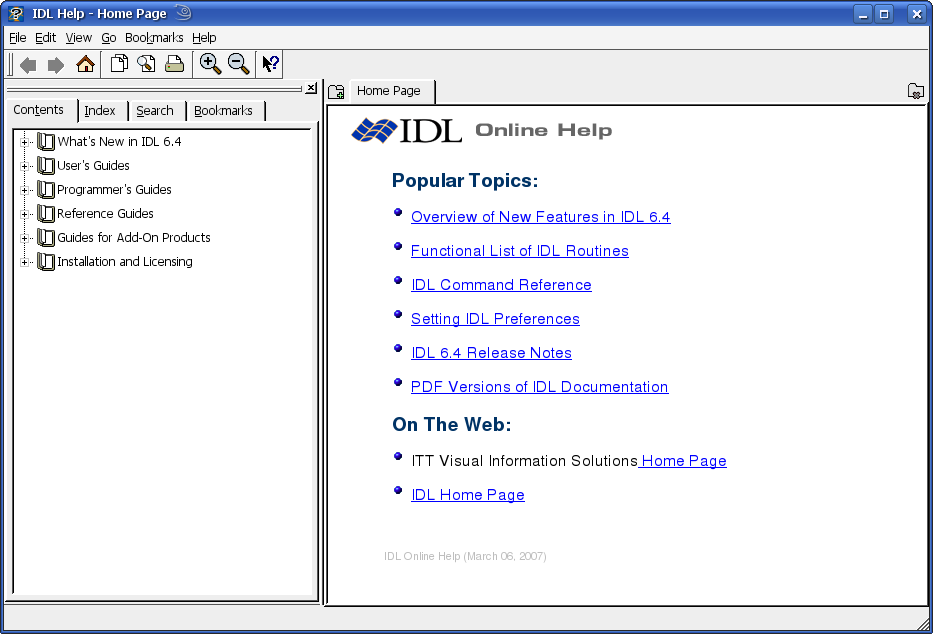
\includegraphics[width=0.8\linewidth]{images/idl_help}
  \end{center}

  The documentation is divided into books aimed at users or developers and
  is fully searchable and cross indexed.

\subsection{Manipulating And Plotting Data}
  Once the data has been loaded from the SDF file we will want to extract
  the specific data we wish to analyse, perhaps perform some mathematical
  operations on it and then plot the results.

  To do this we must learn a few basic essentials about the IDL scripting
  language. Since we are all familiar with the basic concepts shared by
  all computer programming languages, I will just provide a brief overview
  of the essentials and leave other details to the excellent on-line
  documentation.

  IDL supports multidimensional arrays similar to those found in the
  FORTRAN programming language. Whole array operations are supported
  such as \qtt{5*array} to multiply every element of \qtt{array} by $5$.
  Also matrix operations such as addition and multiplication are supported.

  The preferred method for indexing arrays is to use brackets. It is
  possible to use parenthesis instead but this usage is deprecated.
  Column ordering is the same as that used by FORTRAN, so to access
  the $(i,j,k)$th element of an array you would use \qtt{array[i,j,k]}.
  IDL arrays also support ranges so \qtt{array[5:10,3,4]} will return
  a one dimensional array with five elements. \qtt{array[5:*]} specifies
  elements five to $n$ of an $n$ element array. \qtt{array[*,3]} picks
  out the third row of an array.

  There are also a wide range of routines for querying and transforming
  arrays of data. For example, finding minimum and maximum values,
  performing FFTs, etc. These details can all be found by searching the
  on-line documentation. 

  Finally, IDL is a full programming language so you can write your own
  functions and procedures for processing the data to suit your needs.

\subsection{1D Plotting in IDL}
  The most commonly performed plot and perhaps the most useful data analysis
  tool is the 1D plot. In IDL, this is performed by issuing the command
  \cmd{plot,x,y} where \qtt{x} and \qtt{y} are one dimensional arrays of
  equal length. For each element \qtt{x[i]} plotted on the $x$-axis the
  corresponding value \qtt{y[i]} is plotted along the $y$-axis. As a
  simple example:
\begin{boxverbatim}
IDL> plot,[1,2,3],[2,2,5]
\end{boxverbatim}
  Gives rise to the following plot:
  \begin{center}
    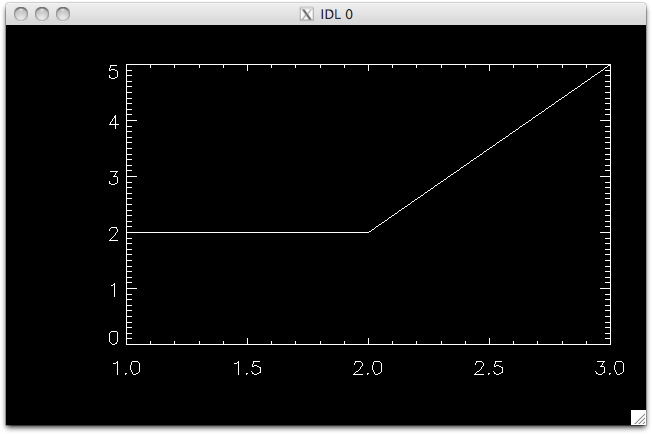
\includegraphics[width=0.7\linewidth]{images/idl_simple_plot}
  \end{center}

  As a more concrete example, we will now take a one-dimensional slice through
  the 2D\linebreak \qtt{Number\_Density} array read in from our SDF data file.
  In this example we will give the $x$ and $y$ axes labels by passing extra
  parameters to the \qtt{plot} routine. A full list of parameters can be found
  in the on-line documentation. In this example we also make use of the
  \qtt{\$} symbol which is IDL's line continuation character.

\begin{boxverbatim}
IDL> data = getdata(0)
IDL> plot,data.x,data.number_density[*,256],xtitle='x', $
IDL>    ytitle='number density'
\end{boxverbatim}
  This command generates the following plot:
  \begin{center}
    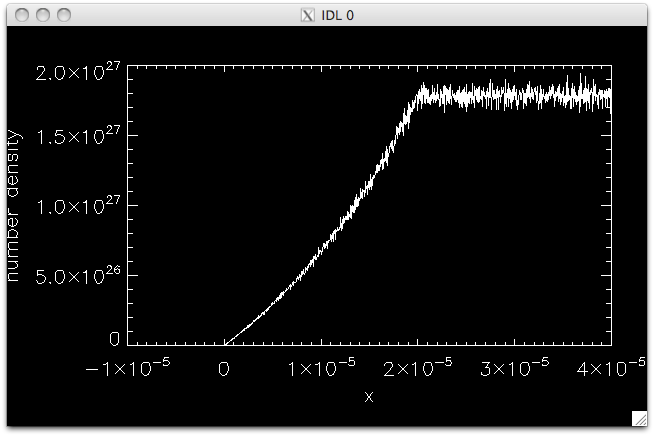
\includegraphics[width=0.7\linewidth]{images/idl_plot}
  \end{center}

\subsection{Postscript Plots}
  The plots shown so far have just been screen-shots of the interactive
  IDL plotting window. These are fairly low quality and could included as
  figures in a paper.

  In order to generate publication quality plots, we must output to the
  postscript device. IDL maintains a graphics context which is set using
  the \cmd{set\_plot} command. The two most commonly used output devices
  are \qtt{x} which denotes the X-server and \qtt{ps} which is the postscript
  device. Once the desired device has been selected, various attributes
  of its behaviour can be altered using the \cmd{device} procedure.
  For example, we can set the output file to use for the postscript plot.
  By default, a file with the name \qtt{idl.ps} is used.

  Note that this file is not fully written until the postscript device is
  closed using the \cmd{device,/close} command. When we have finished our
  plot we can resume plotting to screen by setting the device back to \qtt{x}.

\begin{boxverbatim}
IDL> set_plot,'ps'
IDL> device,filename='out.ps'
IDL> plot,data.x,data.number_density[*,256],xtitle='x', $
IDL>    ytitle='number density',charsize=1.5
IDL> device,/close
IDL> set_plot,'x'
\end{boxverbatim}

  This set of commands results in the following plot being written to
  a file named \qtt{out.ps}.
  \begin{center}
    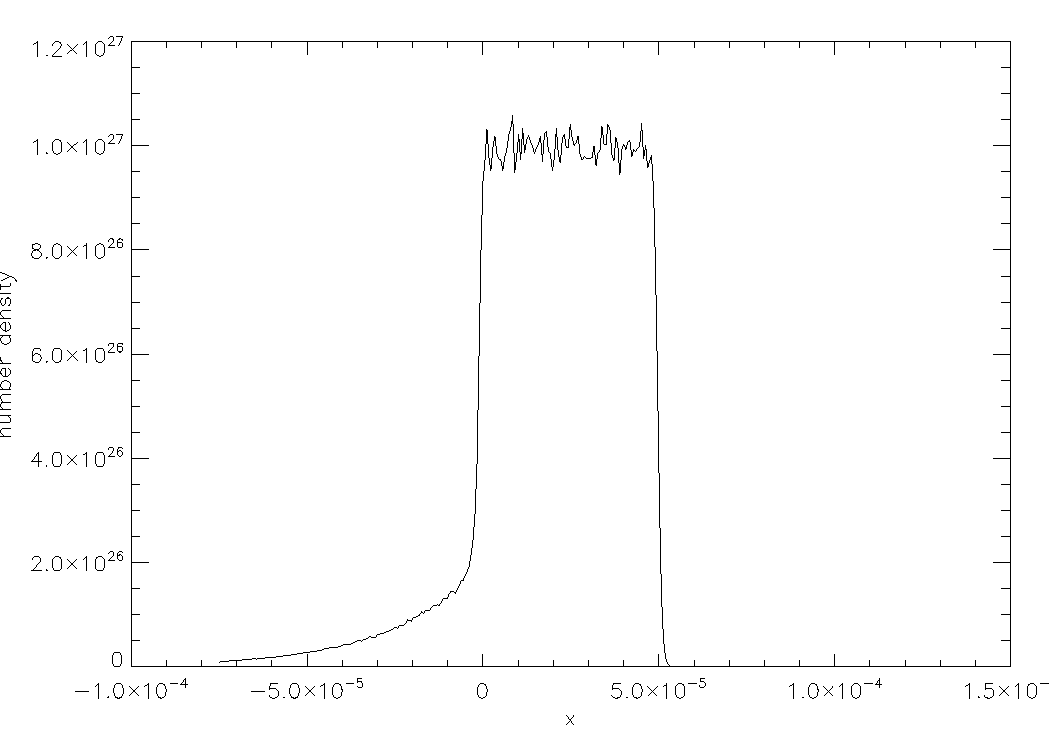
\includegraphics[width=0.8\linewidth]{images/idl_ps_plot}
  \end{center}
  By default, IDL draws its own set of fonts called ``Hershey vector fonts".
  Much better looking results can be obtained by using a postscript font
  instead. These options are passed as parameters to the \cmd{device}
  procedure. More details can be found in the on-line documentation under
  ``Reference Guides $\Rightarrow$ IDL Reference Guide $\Rightarrow$
  Appendices $\Rightarrow$ Fonts".

\subsection{Contour Plots in IDL}
  Whilst 1D plots are excellent tools for quantitive analysis of data,
  we can often get a better qualitative overview of the data using 2D
  or 3D plots.

  One commonly used plot for 2D is the contour plot. The aptly named
  \cmd{contour,z,x,y} procedure takes a 2D array of data values, \qtt{z},
  and plots them against $x$ and $y$ axes which are specified in the
  1D \qtt{x} and \qtt{y} arrays. The number of contour lines to plot is
  specified by the \qtt{nlevels} parameter. If the \qtt{/fill} parameter
  is used then IDL will fill each contour level with a solid colour rather
  than just drawing a line at the contour value.

  The example given below plots a huge number of levels so that a smooth
  looking plot is produced. \qtt{xstyle=1} requests that the $x$ axes drawn
  exactly matches the data in the \qtt{x} variable rather than just using
  a nearby rounded value and similarly for \qtt{ystyle=1}.
\begin{boxverbatim}
IDL> n=100
IDL> levels=max(data.number_density)*findgen(n)/(n-1)
IDL> colors=253.*findgen(n)/(n-1)+1
IDL> contour,data.number_density,data.x,data.y,xstyle=1,ystyle=1, $
IDL>    levels=levels,/fill,c_colors=colors 
\end{boxverbatim}
  Issuing these commands gives us the contour plot shown below. Note that
  the colour table used is not the default one but has been constructed to
  be similar to the one used by VisIt.
  \begin{center}
    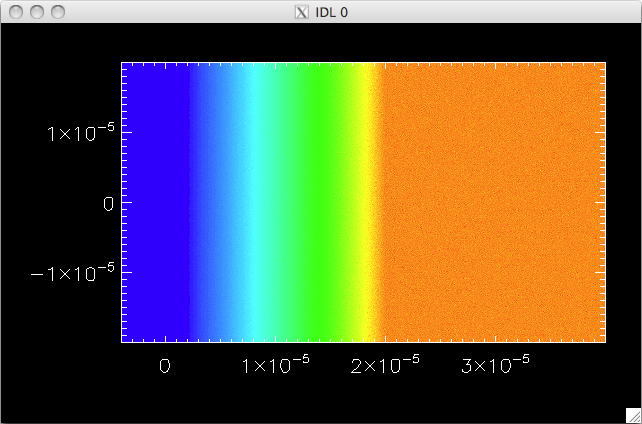
\includegraphics[width=0.8\linewidth]{images/idl_contour}
  \end{center}


\subsection{Shaded Surface Plots in IDL}
  Another method for visualising 2D datasets is to produce a 3D plot in
  which the data is elevated in the $z$ direction by a height proportional
  to its value. IDL has two versions of the surface plot. \cmd{surface}
  produces a wireframe plot and \cmd{shade\_surf} produces a filled and
  shaded one. As we can see from the following example, many of IDL's
  plotting routines accept the same parameters and keywords.

  The first command shown here, \cmd{loadct,3}, asks IDL to load the third
  colour table which is\linebreak ``RED\_TEMPERATURE".

\begin{boxverbatim}
IDL> loadct,3
IDL> shade_surf,data.number_density,data.x,data.y,xstyle=1, $
IDL>    ystyle=1,xtitle='x',ytitle='y',ztitle='number density',charsize=3
\end{boxverbatim}
  \begin{center}
    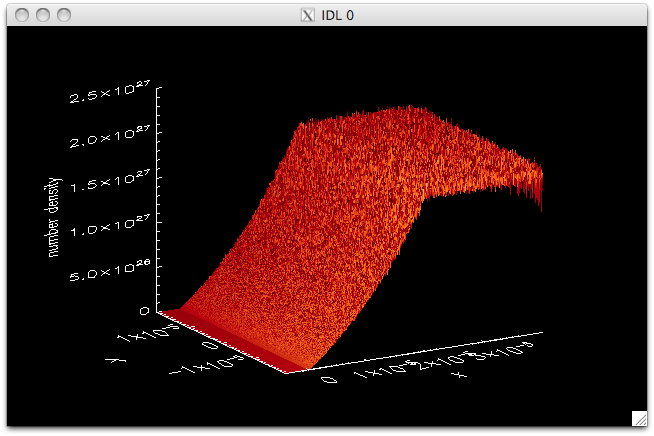
\includegraphics[width=0.8\linewidth]{images/idl_shade_surf}
  \end{center}

\subsection{Interactive Plotting}
  Finally, in recent versions of IDL it is now possible to perform all of
  these plot types in an interactive graphical user interface. The corresponding
  procedures are launched with the commands \cmd{iplot}, \cmd{icontour}
  and \cmd{isurface}.

\begin{boxverbatim}
IDL> iplot,data.x,data.number_density[*,256]
\end{boxverbatim}
  \begin{center}
    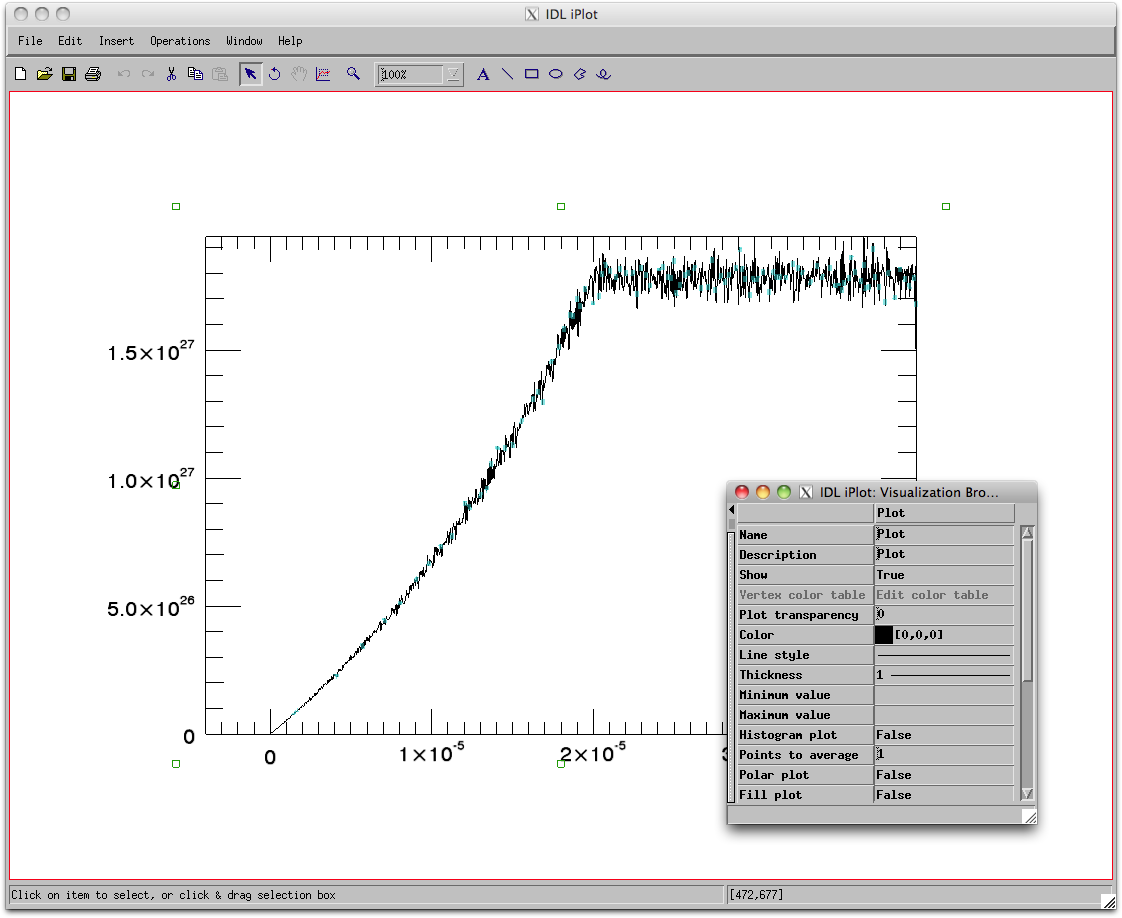
\includegraphics[width=0.8\linewidth]{images/idl_iplot}
  \end{center}

  IDL is an extremely useful tool but it also comes with a fairly hefty
  price tag. If you are not part of an organisation that will buy it for
  you then you may wish to look into a free alternative. It is also a
  proprietary tool and you may not wish to work within the restrictions
  that this imposes.

  There are a number of free tools available which offer similar functionality
  to that of IDL, occasionally producing superior results.

  For a simple drop-in replacement, the GDL project aims to be fully compatible
  and works with the existing {\EPOCH} IDL libraries after a couple of small
  changes. Other tools worth investigating are {\em ``yorick"} and
  {\em ``python"} with the {\em ``SciPy"} libraries. At present there is
  no SDF reader for either of these utilities but one may be developed if
  there is sufficient demand.

\section{Using VisIt to visualise data}

\subsection{LLNL VisIt}
LLNL's VisIt software is a parallel data visualisation package
(\inlinecode{https://wci.llnl.gov/codes/visit/}). {\EPOCH} comes with source
code for the plug-in needed to allow VisIt to load the SDF output files which
are generated by {\EPOCH}. There are full manuals for VisIt which can be
downloaded from the above link so no further details will be given here. To
build the plug-in, first ensure that the visit binary is in the \$PATH
environment variable. Then simply type ``make visit'' in one of the
\inlinecode{epoch\{1,2,3\}d} directories.
For more experienced
users of VisIt, the xml file which is used to generate the plug-in is supplied
in the VisIt subdirectory, called \inlinecode{SDF2.xml}.

  Whilst IDL is an excellent tool for visualising 1D and 2D datasets, it
  is extremely poor when it comes to dealing with 3D data. For this purpose,
  we recommend the use of the {\em ``VisIt"} visualisation tool.

  The other great advantage that VisIt has over IDL is the ability to
  render in parallel, enabling the visualisation of huge datasets which
  IDL would be incapable of dealing with.

  \begin{itemize}
  \item
    Initially developed by the Department of Energy (DOE) Advanced Simulation
    and Computing Initiative (ASCI) 
  \item
    Now developed and maintained by the Lawrence Livermore National Laboratory
    along with a group of external contributors
  \item
    Written in C++ and supports python and Java interfaces
  \item
    Available for UNIX (Irix, Tru64, AIX, Linux, Solaris), Mac OS X
    (10.3, 10.4), and Windows platforms
  \item
    Open source and freely available under the BSD license
  \item
    Plots, operators and database readers are implemented as plugins allowing
    the VisIt to be dynamically extended at run-time
  \item
    Powerful set of tools for manipulating, analysing and visualising 3D
    datasets
  \item
    Parallel and distributed architecture for visualising huge data sets
  \end{itemize}

\subsection{Obtaining And Installing VisIt}
  Both the source code and pre-compiled binaries are available for download
  from the projects web page which is found at the URL
  {\tt https://wci.llnl.gov/codes/visit/home.html}

  \begin{center}
    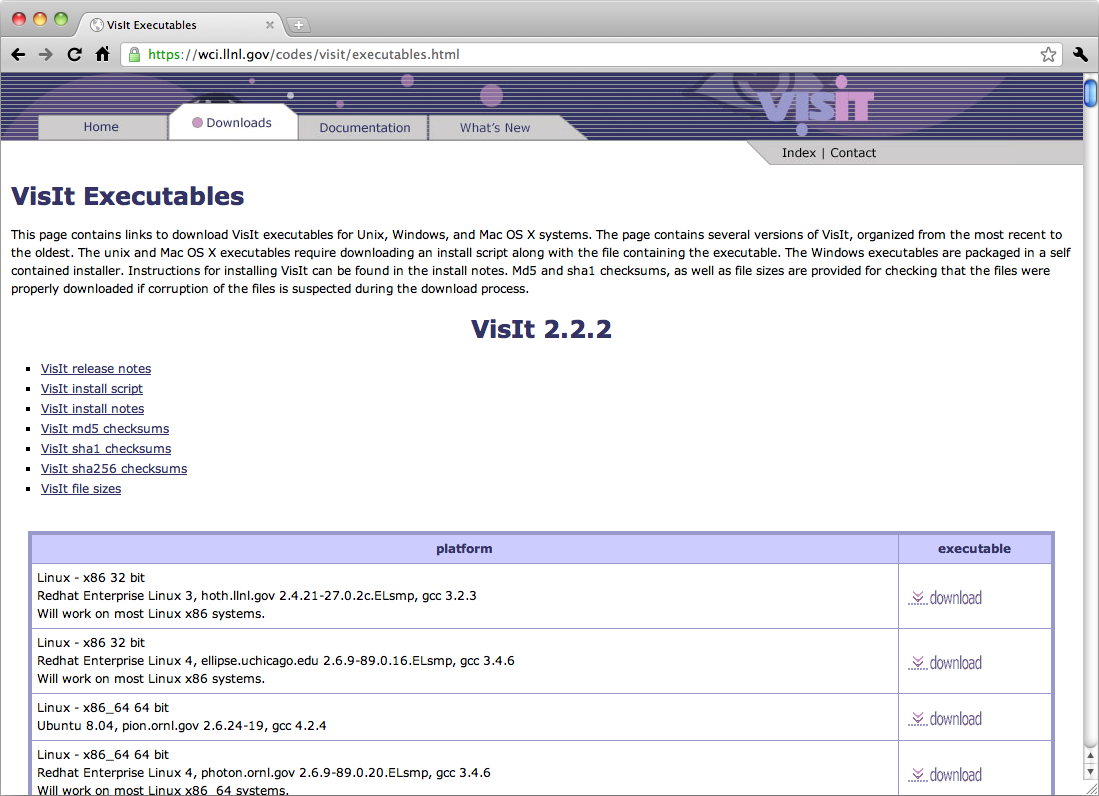
\includegraphics[width=0.8\linewidth]{images/visit_web}
  \end{center}

  There are full instructions for compiling the project from source code
  along with build scripts written to help ease the process. However, this
  is not recommended as it is an extremely large tool and the compilation
  takes hours to complete. It is usually far easier to download a pre-compiled
  binary which matches your system architecture.

  However, occasionally compilation may be a necessary step. Linux
  in particular is a moving target and it is not always possible to
  find a binary which matches the particular combination of libraries
  installed on your system.

  The easiest way to install the VisIt tool is to ask the system
  administrator to do it for you. However, this may not always be the
  best option. The system in question may be run by someone who is
  not concerned with your particular software needs or has insufficient
  skills to deal with the task. In any case, VisIt has a fairly rapid
  release schedule and you may find that some functionality you need
  is not present in the version installed on the machine.

  Fortunately, for all these scenarios it is usually quite easy to install
  a copy in your own home directory. Just find a binary on the web page
  {\tt https://wci.llnl.gov/codes/visit/executables.html} which closely
  matches your machine and download it. This can be unpacked into your
  home directory with the command
  \cmd{tar xzf visit2\_2\_2.linux-x86\_64.tar.gz}. The actual name of
  the file will vary depending on which version you downloaded. This
  will unpack the VisIt binary into a subdirectory named \txt{visit/}.
  Now all that is necessary is to add this to your search path.
  eg. \cmd{export PATH=\$HOME/visit/bin:\$PATH}

  These instructions illustrate the steps required for installing your
  own copy of VisIt when you have no other choice. VisIt is an extremely
  large program, so if a version is already available then it is usually
  better to use the installed version.

  The machines at Warwick have a recent version of VisIt installed which
  is available via the \qtt{modules} system. To make use of it you must
  first issue the command \cmd{module load visit}.

\subsection{Compiling The Reader Plugin}

  One piece of compilation which is almost always necessary is that of
  the SDF reader plugin. This is shipped as source code in a subdirectory
  of the {\EPOCH} repository. It is located in the \txt{VisIt/} subdirectory
  of the main \txt{epoch/} directory. The reader will work for any
  SDF file generated by any code which uses the SDF I/O routines. You do
  not need a separate reader for each version of {\EPOCH}.

  To compile, first navigate to one of the \txt{epoch*d/} directories in your
  {\EPOCH} repository. Just type ``make visit'' and the build scripts should
  take care of the rest.
  The SDF reader plugin will be installed into the directory
  \txt{\$HOME/.visit/linux-intel/plugins/databases/} on your system.
  Note that the \txt{linux-intel/} component will vary depending on
  your machine operating system and architecture.

  Each time you install a new version of VisIt you must recompile the reader
  to match the new installation. It will also occasionally be necessary to
  recompile when changes occur to the SDF data format or the reader plugin
  itself. The developers will notify users if this is the case, although
  it does no harm to regularly recompile the reader as a matter of course.

  We will see later that it is possible to do remote data visualisation
  with VisIt in which the GUI is launched and interacted with on one
  machine and the data files are located on a separate machine entirely.
  In this situation the reader must be installed on the remote machine and
  must match the setup there. The setup on the local machine is unimportant.
  In fact it is not even necessary to have the plugin installed on the
  local machine. This is particularly useful when using a Windows environment
  to analyse data located on a remote UNIX workstation.

\subsection{Loading Data Into VisIt}
  \begin{center}
    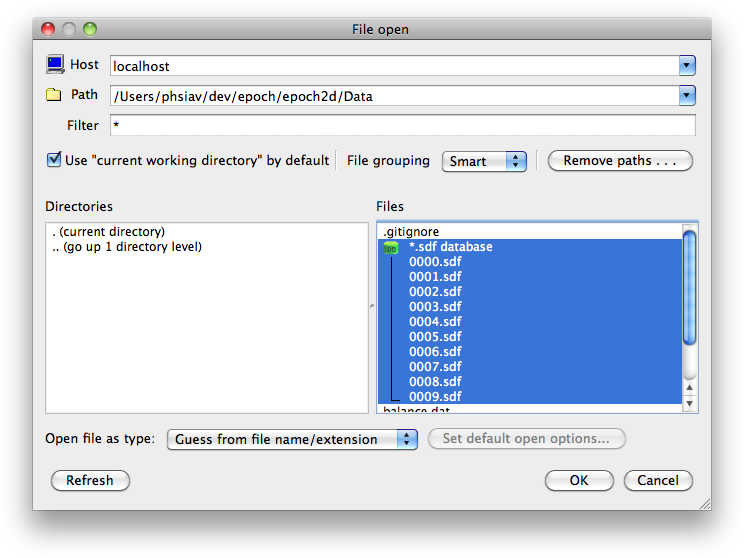
\includegraphics[width=0.8\textwidth]{images/visit_db_list}
  \end{center}

  The most straightforward method for loading data into VisIt is to
  start the application and then browse the filesystem for the dataset
  you are interested in. This is done by selecting \qm{File $\Rightarrow$
  Open file} from the VisIt menu bar. A file selection dialogue will appear
  allowing you to browse directories along with the options to filter
  the results according to a given regular expression and grouping options.
  By default, VisIt will attempt to group all files containing the same
  suffix and some kind of numbering system into a sort of virtual database.

  The right-hand pane of this window shows a list of selected files which
  will appear in the main VisIt window when you are finished.

  An alternative method of specifying the data file to open is to pass
  a command line option when the tool is launched. An example of this
  method is \cmd{visit -o Data/0000.sdf}. When the file is specified in
  this manner the list of files shown in the VisIt window will also
  include the full list of files in the dataset's subdirectory and
  all the files in the current working directory. The other SDF files
  will be grouped together in a virtual database.

  Yet another method for selecting the dataset to use is by opening a
  previously saved session file. Will discuss this further in a later section

  \begin{center}
    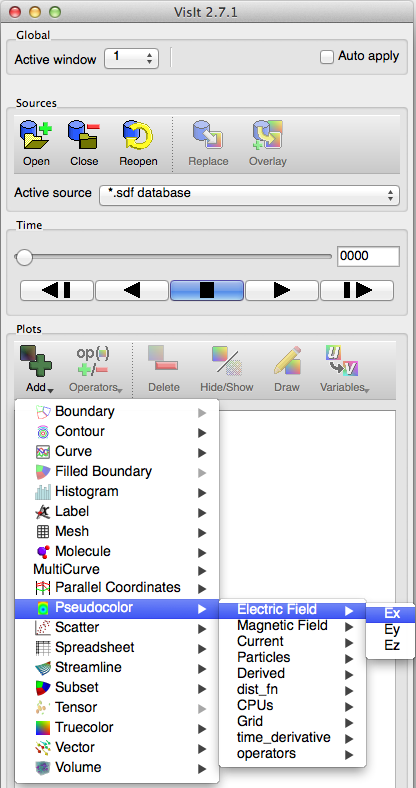
\includegraphics[height=0.7\textheight]{images/visit_select_var}
  \end{center}
  Once a SDF file has been successfully loaded the \qm{Add} menu item
  will become un-greyed and the cycle numbers for each file in the virtual
  database will be displayed. If we navigate to one of the plot types we
  are able to select the variable to plot from a drop-down list.

\subsection{Contour Plots in VisIt}
  We will now replicate each of the plots which we generated using IDL
  in earlier sections. For reasons which will soon become clear we begin
  with the contour plot and move on to the 1D plot in the next section.

  Having opened the same dataset we were using in the IDL discussion we
  now select the \qm{Add} menu item. Notice that many of the plot
  types listed here are greyed out and cannot be selected. This is because
  many of the plots are dependent on the type or dimensionality of the
  variable to be plotted. If our dataset contains no variables which match
  the required properties for a plot, the plot menu will be disabled.

  For the current dataset there is no \qm{Boundary} plot available since this
  requires multi-material data and none of our variables meet
  that criteria.

  The list contains a menu item for a \qm{Contour} plot. We are not going
  to select this item since it only generates a contour plot with lines
  indicating each contour level and not a filled version. Instead we
  choose \qm{Add $\Rightarrow$ Pseudocolor $\Rightarrow$ Derived $\Rightarrow$
  Number\_Density} and then hit the \qm{Draw} button.
  \begin{center}
    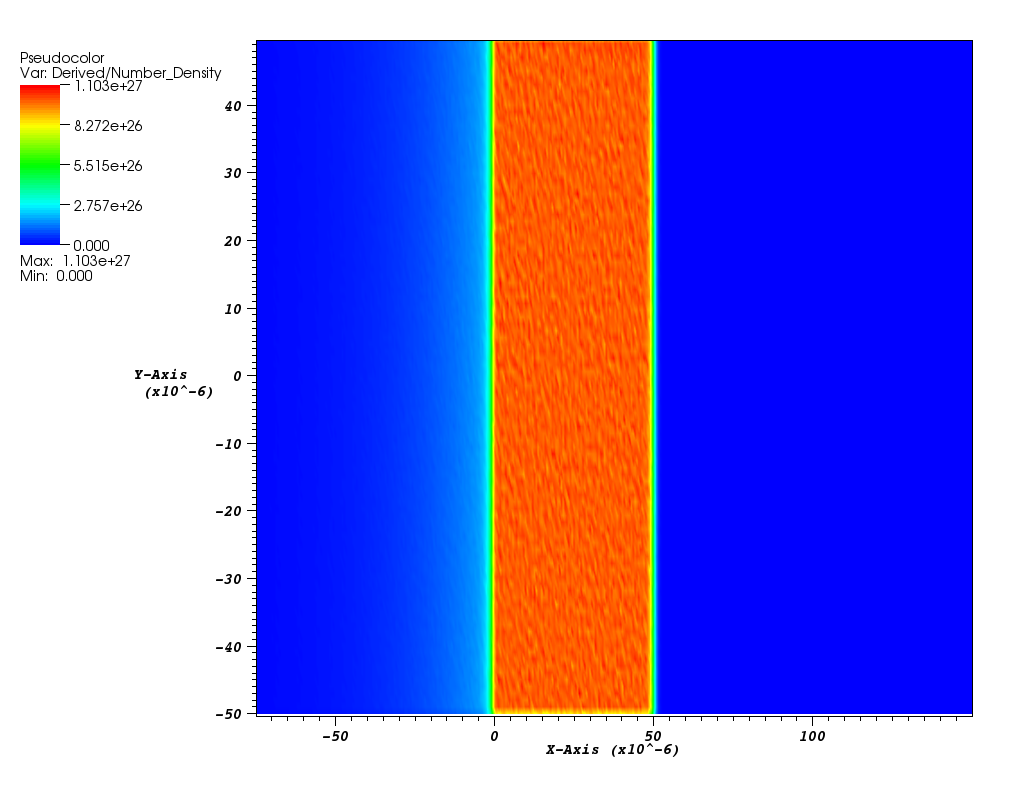
\includegraphics[width=0.8\linewidth]{images/visit_contour}
  \end{center}

  There are many settings which can alter the visual appearance
  of plots generated by VisIt. The first point of call is usually to
  open up the \qm{Plot Attributes} or \qm{Operator Attributes} dialogue
  corresponding to the
  plot in question. A simpler method for accomplishing this task is
  to double-click on the plot in the main VisIt menu pane which will
  launch the corresponding \qm{Plot Attributes} dialogue.

  If it is the operator attributes you wish to change,
  click on the white arrow on the left hand side of the plot in the
  main VisIt menu pane. This will drop down to reveal a list containing
  the plot and all operators acting on it. Double-clicking on an operator
  will launch the corresponding \qm{Operator Attributes} dialogue.
  \begin{center}
    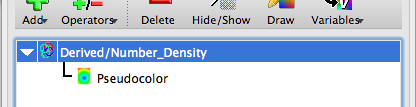
\includegraphics[width=0.7\linewidth]{images/visit_attrib}
  \end{center}

  Another important tool for controlling the appearance of plots can
  be found in \qm{Controls $\Rightarrow$ Annotation} from the VisIt menu
  bar. This allows all of the plot annotations to be modified such as
  the legend, title, axis labels, etc.
  \begin{center}
    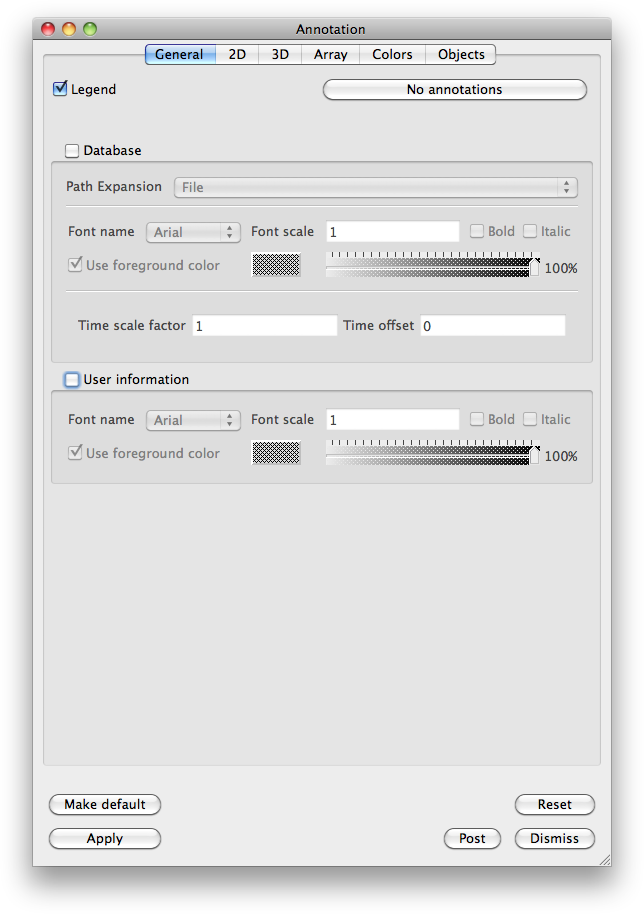
\includegraphics[width=0.6\linewidth]{images/visit_annot}
  \end{center}

\subsection{1D Plotting in VisIt}
  A 1D plot in VisIt is called a \qm{Curve} plot. We already mentioned that
  this was greyed out because we have no one dimensional variables in our
  data file.

  The solution to this dilemma is the lineout operator which extracts a
  one dimensional array from a 2D or 3D variable. This operator is selected
  by pressing the button with red and blue lines located at the top of
  the plot window.
  \begin{center}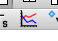
\includegraphics{images/visit_lineout}\end{center}

  Once the button has been pressed, we can click and drag anywhere in
  the \qm{Pseudocolor} plot window. When we release the mouse button a
  new plot window pops up containing a \qm{Curve} plot of the data just
  selected.
  \begin{center}
    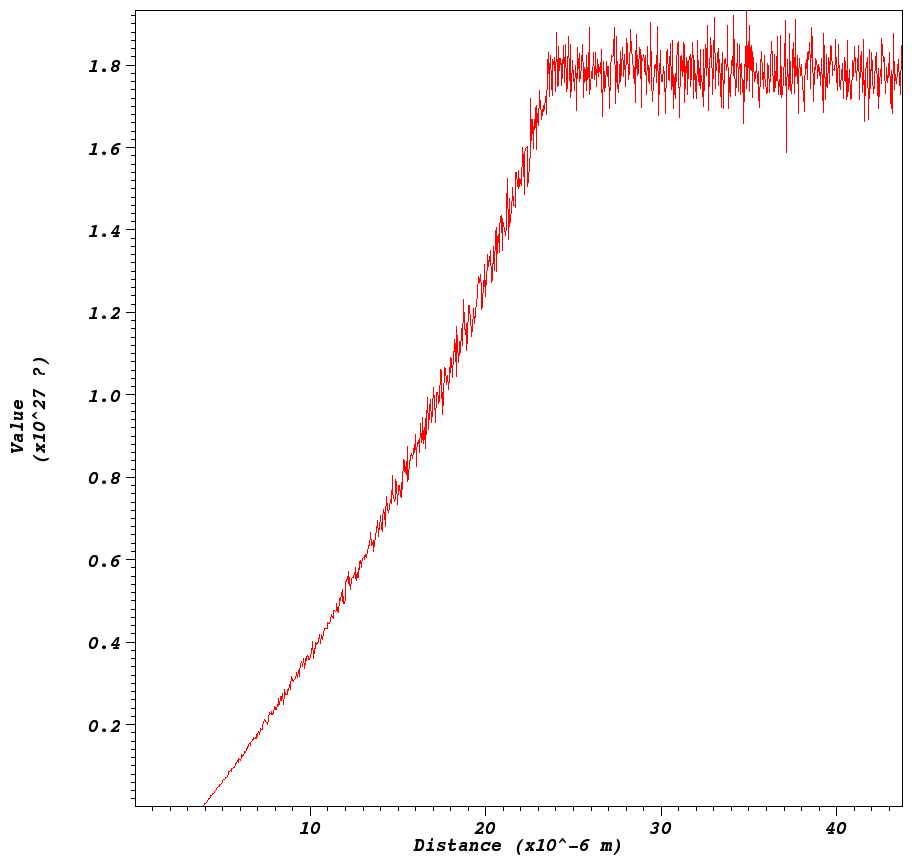
\includegraphics[width=0.8\linewidth]{images/visit_curve}
  \end{center}

  In order to change the attributes for this plot, we must first select
  \qm{Active window} number 2 in the main VisIt pane.

\subsection{Shaded Surface Plots in VisIt}
  Again, we will confusingly refuse to pick the obvious plot type for this
  task. There is \qm{Surface} plot listed in the menu. However, most of the
  time the \qm{Elevator} operator does what we want and also gives us more
  flexibility.

  The first step is to do a \qm{Pseudocolor} plot of \qm{Number\_Density} as
  we did before. Next select the \qm{OpAtts $\Rightarrow$ Elevate} menu item.
  In the pop up dialogue click on the \qm{Elevation height relative to XY
  limits} and then \qm{Apply}. Click \qm{Yes} when the warning dialogue pops
  up.
  \begin{center}
    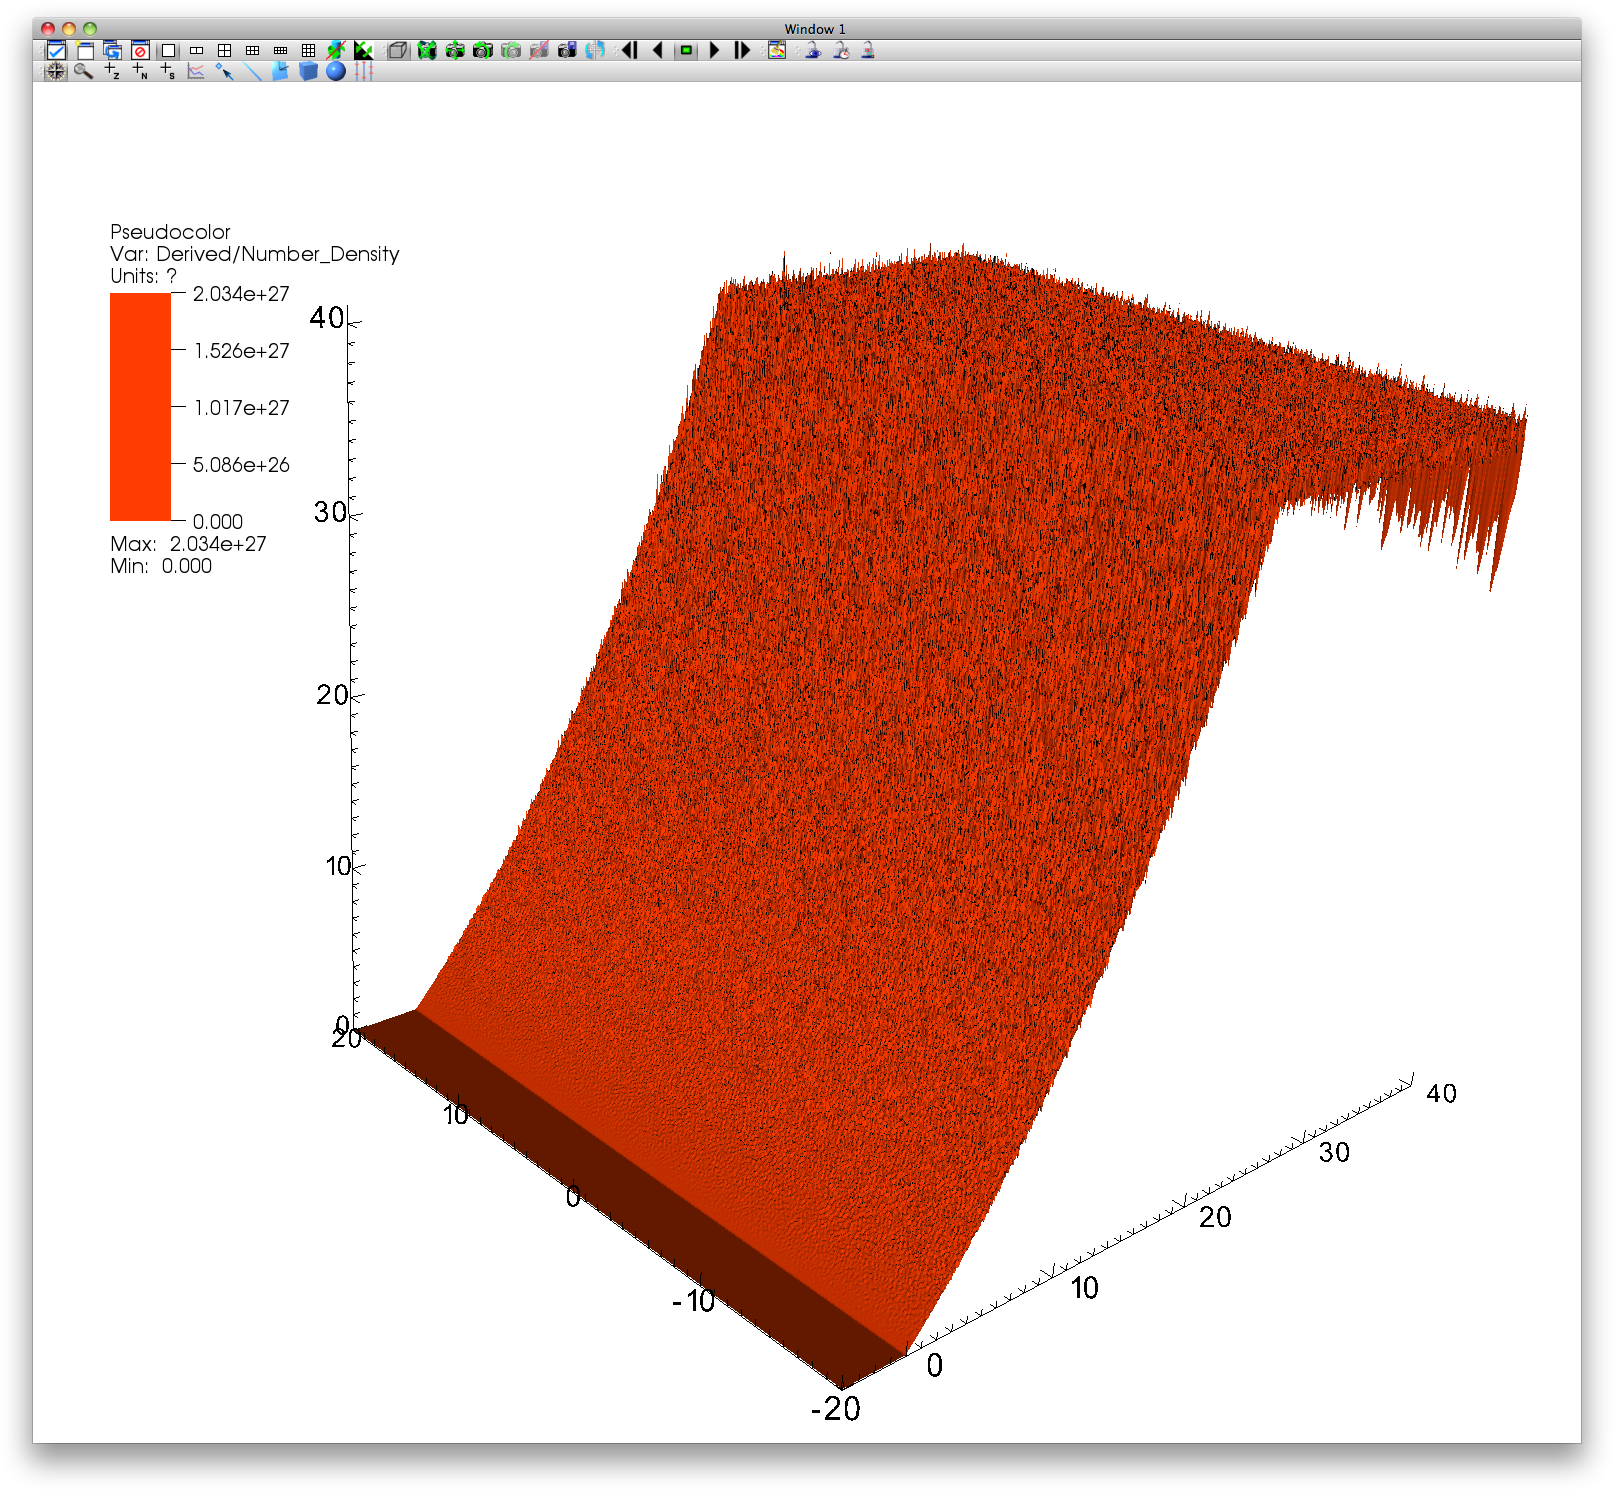
\includegraphics[width=0.8\linewidth]{images/visit_shade_surf}
  \end{center}

  To make this plot look similar to the one generated by IDL, we have changed
  the colour table using \qm{Controls $\Rightarrow$ Color table}.
  We also changed the axis appearance with the annotations menu discussed
  earlier and changed the height of the elevation using the min and max
  operator attributes.

\subsection{Creating User-Defined Expressions}
  VisIt comes with an extremely powerful method of manipulating data before
  visualising the results. The basic idea is that an array is transformed
  by applying a set of mathematical functions on all its elements and then
  the result is defined as a new variable. Once defined, this variable
  behaves in exactly the same way as any of the variables read from the
  data file.

  As an example, we can combine the three components of electric field
  to generate a single electric field vector.
  \begin{center}
    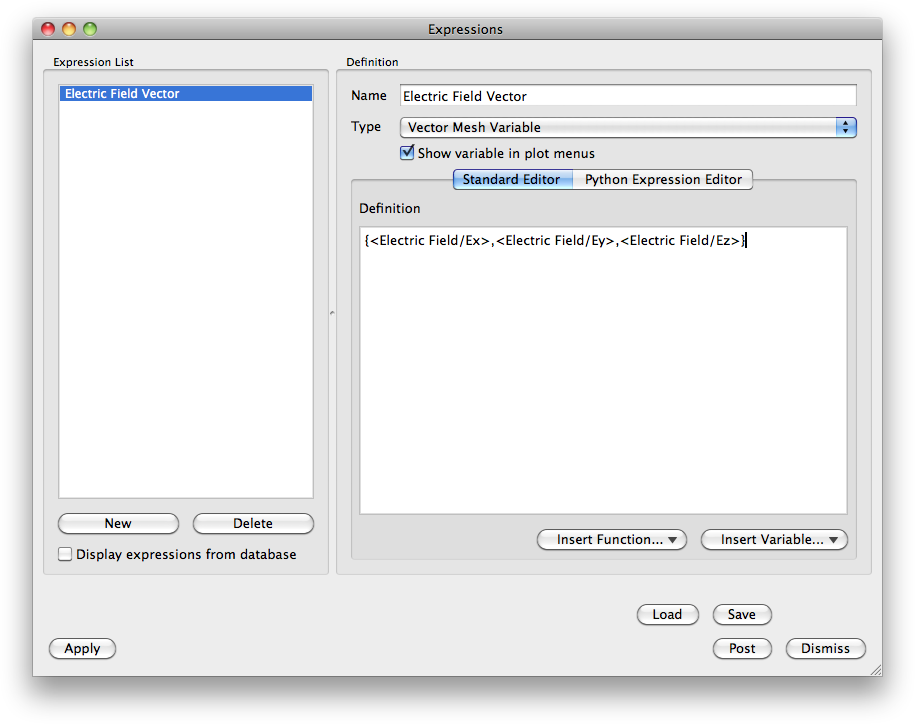
\includegraphics[width=0.8\linewidth]{images/visit_expression_vector}
  \end{center}

  Now when we return to the \qm{Add} menu we see that the \qm{Vector}
  and \qm{Streamline} plot types now have an entry for our newly defined
  vector.

\subsection{Creating Movies}
  A compelling visualisation of numerically generated data is often made
  by combining a series of images into a movie. This can be an invaluable
  method for illustrating the basic behaviour of a system as it changes
  over time. Alternatively rotating around a 3D scene can sometimes
  give a much better idea of the structure in the model being presented. 
  There can also be much to gain by constructing visual fly-throughs
  of a scene, dynamically slicing through sets of data or combinations
  of all these techniques.

  VisIt provides several facilities for generating movies from your
  data. The simplest of these is to select the \qm{File $\Rightarrow$
  Save movie} menu item. This pops up a movie wizard which will walk
  you through the process of generating a simple linear movie based
  on the time-advancing snapshots represented by your virtual database
  of files. Alternatively you can select one of the pre-defined movie
  templates which manipulate the currently selected plot and create
  a movie from that.

  Creating a simple time advancing movie is as simple as walking through
  the wizard dialogue and selecting from the self-explanatory options
  presented to you.

  For many uses, the wizard will give exactly the desired results. However
  it is occasionally useful to have a little more control over how the
  movie is created. In such cases it can be useful to specify an image
  format such as \qm{PNG} to save to rather than \qm{MPEG}. VisIt will
  then generate one image per frame and number them consecutively. At
  the end of the process the images can be converted into a movie using
  whatever tool best accomplishes the task.

  \begin{center}
    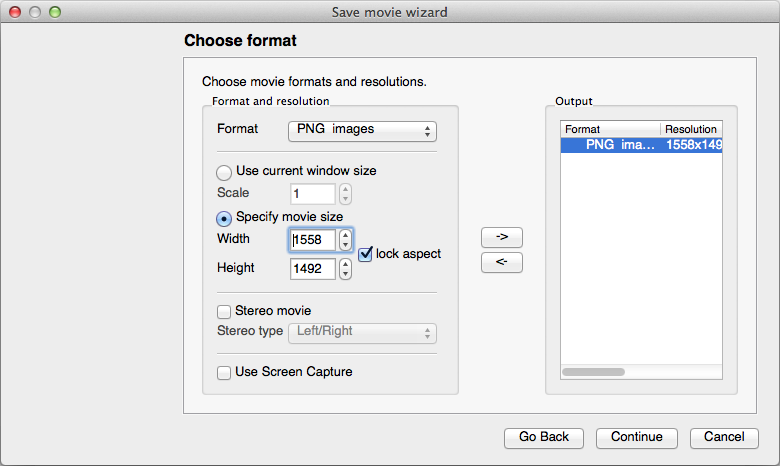
\includegraphics[width=0.8\linewidth]{images/visit_movie}
  \end{center}
  Another useful tip is to select the \qm{Later, tell me the command to
  run} radio button. This will output a long command which can run from
  a UNIX terminal screen. The advantage is that no X session is required
  so the command can be run in the background. It also becomes a simple
  task to interrupt the job at any point and resume it from where it
  left off at a later date. In a similar manner it is easy to resume
  a job which crashes half way through for any reason.

  More complex movies can be created by using VisIt's keyframing facility
  which allows you to change animation attributes such as view or plot
  attributes as the animation progresses. Further information about this
  somewhat complex task can be found in the on-line help.

  Finally, you can use VisIt's python scripting interface to programmatically
  describe the details of each frame as the movie progresses. This approach
  offers far more flexibility in what can be achieved but is also much
  more involved and time consuming than the previous two methods. Again,
  further information on this subject can be found in the on-line help
  system.

\subsection{Remote Visualisation}
  It was mentioned earlier that it is possible to perform remote visualisation
  using VisIt. This is a process in which the data files being interrogated
  reside on a different machine to the one on which the VisIt GUI runs and
  where the results are plotted.

  This method of working can be extremely useful when the data is generated
  on a powerful machine located in an external environment such as a large
  cluster. Another common use is when {\EPOCH} is executed on a UNIX machine
  and the desktop used for visualisation is running Windows.

  It is sometimes possible to run a graphical tool on the remote machine
  and tunnel the X-server session through to the local machine but this
  can be quite slow and unstable. When connecting to a remote VisIt
  instance the only data which needs to be sent between machines is the
  pre-rendered image and a few simple plotting commands. Naturally, this
  can be a {\em much} faster approach.

  Also, as mentioned before, it is possible to use a machine on which the
  reader plugin is difficult or impossible to compile for and connect
  to a machine on which the reader is already installed.

  In order to use the remote visualisation facility, you must first
  set up a \qm{Host Profile} for the remote machine using the \qm{Options
  $\Rightarrow$ Host Profiles} menu item. The pre-compiled binaries are
  shipped with a long list of pre-defined host profiles. These are unnecessary
  for anyone not affiliated and can safely be removed by deleting the
  directory \txt{\$HOME/visit/current/.visit/} (assuming you have unpacked
  the VisIt tarball into your home directory).

  \begin{center}
    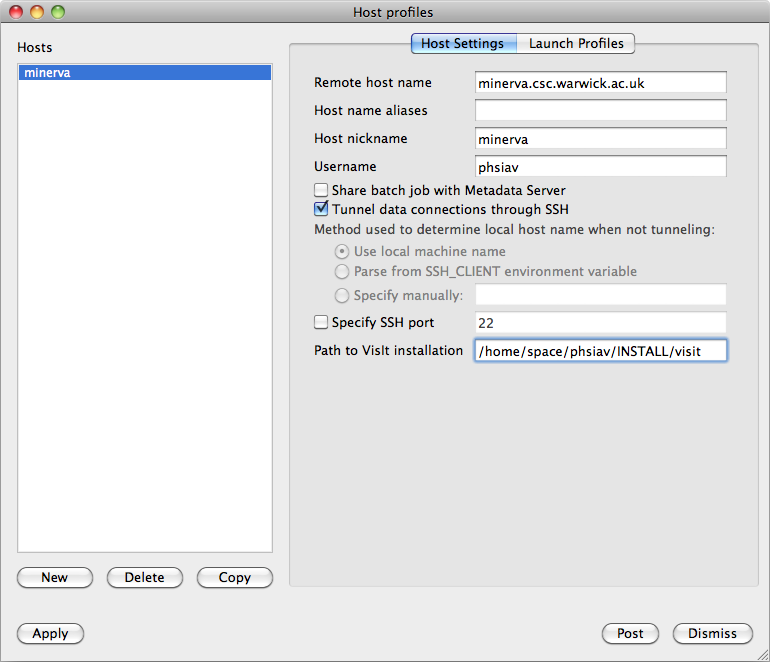
\includegraphics[width=0.8\linewidth]{images/visit_host_profile}
  \end{center}

  Create a new profile by clicking on the \qm{New profile} button and filling
  out some of the form fields. The important ones to change are \qm{Profile
  name}, \qm{Remote host name}, \qm{Host name aliases} and \qm{Username}.
  If the visit binary is not in your default search path on the remote
  machine then you must specify its location by passing \qm{-dir
  /base/installpath/visit} to \qm{Additional options}.

  Now select the \qm{Options $\Rightarrow$ Save Settings} menu item to
  ensure that the profile is saved for future sessions.

  Data on the remote machine can now be loaded by selecting \qm{File
  $\Rightarrow$ Open file} and picking the desired host profile
  from the drop down list of \qm{Hosts}. VisIt will wait for the
  remote process to launch and then continue with the file selection
  procedure but now displaying files located on the remote machine
  rather than the local one. From this point on everything should work
  as before except you should see the name of the remote machine in the
  \qm{Selected files} dialogue. 

  \begin{center}
    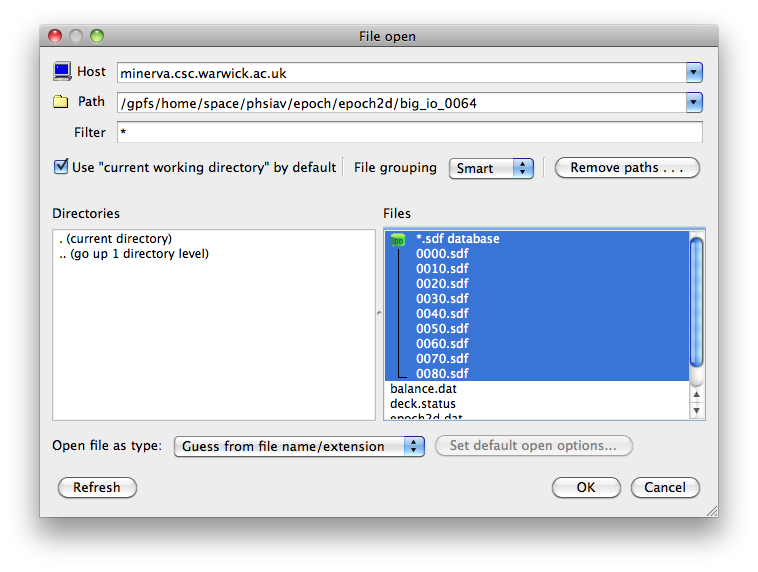
\includegraphics[width=0.8\linewidth]{images/visit_host_files}
  \end{center}

\subsection{Parallel Visualisation}
  Before reading this section be warned that the current version of
  the SDF reader is not capable of reading data in parallel! However,
  this is high on the list of issues to be addressed so a parallel
  version ought to be released some time in the near future.

  Parallel visualisation is performed in almost exactly the same manner
  as remote visualisation. Again, you must create a host profile for the
  purpose except this time you need to check the \qm{Parallel computation
  engine} radio button. This will activate a \qm{Parallel options} tab
  which must be filled in to match the cluster on which the job will
  be launched.

  The major difference now is due to the fact that VisIt must be launched
  by an external job script which fits in with the queueing system used
  by the parallel machine. Usually you will need to consult with the
  system administrator of the cluster to confirm which launch method and
  arguments to use.

  The details of job launch can be better understood by reading through
  the file\linebreak \txt{\$HOME/visit/current/bin/internallauncher}. This is
  a bash script which parses the arguments and executes the specified
  launch method.
%\subsection{Examples}
%  \begin{itemize}
%  \item
%  \end{itemize}
%\section*{Summary}
%
%\begin{frame}{Summary}
%
%  % Keep the summary *very short*.
%  \begin{itemize}
%  \item
%    Item 1
%  \end{itemize}
%\end{frame}



\end{document}
